% Generated by Sphinx.
\def\sphinxdocclass{report}
\documentclass[a4paper,12pt,oneside]{sphinxmanual}
\usepackage[utf8x]{inputenc}
\usepackage{cmap}
\usepackage[T1]{fontenc}
\usepackage[russian]{babel}
\usepackage{times}
\usepackage[Sonny]{fncychap}
\usepackage{longtable}
\usepackage{sphinx}
\usepackage{multirow}
\setkeys{Gin}{width=.80\textwidth}

\title{Blend4Web. User manual}
\date{April 14, 2014}
\release{14.03.28}
\author{Triumph LLC}
\newcommand{\sphinxlogo}{}
\renewcommand{\releasename}{Release}
\makeindex

\makeatletter
\def\PYG@reset{\let\PYG@it=\relax \let\PYG@bf=\relax%
    \let\PYG@ul=\relax \let\PYG@tc=\relax%
    \let\PYG@bc=\relax \let\PYG@ff=\relax}
\def\PYG@tok#1{\csname PYG@tok@#1\endcsname}
\def\PYG@toks#1+{\ifx\relax#1\empty\else%
    \PYG@tok{#1}\expandafter\PYG@toks\fi}
\def\PYG@do#1{\PYG@bc{\PYG@tc{\PYG@ul{%
    \PYG@it{\PYG@bf{\PYG@ff{#1}}}}}}}
\def\PYG#1#2{\PYG@reset\PYG@toks#1+\relax+\PYG@do{#2}}

\expandafter\def\csname PYG@tok@gd\endcsname{\def\PYG@tc##1{\textcolor[rgb]{0.63,0.00,0.00}{##1}}}
\expandafter\def\csname PYG@tok@gu\endcsname{\let\PYG@bf=\textbf\def\PYG@tc##1{\textcolor[rgb]{0.50,0.00,0.50}{##1}}}
\expandafter\def\csname PYG@tok@gt\endcsname{\def\PYG@tc##1{\textcolor[rgb]{0.00,0.27,0.87}{##1}}}
\expandafter\def\csname PYG@tok@gs\endcsname{\let\PYG@bf=\textbf}
\expandafter\def\csname PYG@tok@gr\endcsname{\def\PYG@tc##1{\textcolor[rgb]{1.00,0.00,0.00}{##1}}}
\expandafter\def\csname PYG@tok@cm\endcsname{\let\PYG@it=\textit\def\PYG@tc##1{\textcolor[rgb]{0.25,0.50,0.56}{##1}}}
\expandafter\def\csname PYG@tok@vg\endcsname{\def\PYG@tc##1{\textcolor[rgb]{0.73,0.38,0.84}{##1}}}
\expandafter\def\csname PYG@tok@m\endcsname{\def\PYG@tc##1{\textcolor[rgb]{0.13,0.50,0.31}{##1}}}
\expandafter\def\csname PYG@tok@mh\endcsname{\def\PYG@tc##1{\textcolor[rgb]{0.13,0.50,0.31}{##1}}}
\expandafter\def\csname PYG@tok@cs\endcsname{\def\PYG@tc##1{\textcolor[rgb]{0.25,0.50,0.56}{##1}}\def\PYG@bc##1{\setlength{\fboxsep}{0pt}\colorbox[rgb]{1.00,0.94,0.94}{\strut ##1}}}
\expandafter\def\csname PYG@tok@ge\endcsname{\let\PYG@it=\textit}
\expandafter\def\csname PYG@tok@vc\endcsname{\def\PYG@tc##1{\textcolor[rgb]{0.73,0.38,0.84}{##1}}}
\expandafter\def\csname PYG@tok@il\endcsname{\def\PYG@tc##1{\textcolor[rgb]{0.13,0.50,0.31}{##1}}}
\expandafter\def\csname PYG@tok@go\endcsname{\def\PYG@tc##1{\textcolor[rgb]{0.20,0.20,0.20}{##1}}}
\expandafter\def\csname PYG@tok@cp\endcsname{\def\PYG@tc##1{\textcolor[rgb]{0.00,0.44,0.13}{##1}}}
\expandafter\def\csname PYG@tok@gi\endcsname{\def\PYG@tc##1{\textcolor[rgb]{0.00,0.63,0.00}{##1}}}
\expandafter\def\csname PYG@tok@gh\endcsname{\let\PYG@bf=\textbf\def\PYG@tc##1{\textcolor[rgb]{0.00,0.00,0.50}{##1}}}
\expandafter\def\csname PYG@tok@ni\endcsname{\let\PYG@bf=\textbf\def\PYG@tc##1{\textcolor[rgb]{0.84,0.33,0.22}{##1}}}
\expandafter\def\csname PYG@tok@nl\endcsname{\let\PYG@bf=\textbf\def\PYG@tc##1{\textcolor[rgb]{0.00,0.13,0.44}{##1}}}
\expandafter\def\csname PYG@tok@nn\endcsname{\let\PYG@bf=\textbf\def\PYG@tc##1{\textcolor[rgb]{0.05,0.52,0.71}{##1}}}
\expandafter\def\csname PYG@tok@no\endcsname{\def\PYG@tc##1{\textcolor[rgb]{0.38,0.68,0.84}{##1}}}
\expandafter\def\csname PYG@tok@na\endcsname{\def\PYG@tc##1{\textcolor[rgb]{0.25,0.44,0.63}{##1}}}
\expandafter\def\csname PYG@tok@nb\endcsname{\def\PYG@tc##1{\textcolor[rgb]{0.00,0.44,0.13}{##1}}}
\expandafter\def\csname PYG@tok@nc\endcsname{\let\PYG@bf=\textbf\def\PYG@tc##1{\textcolor[rgb]{0.05,0.52,0.71}{##1}}}
\expandafter\def\csname PYG@tok@nd\endcsname{\let\PYG@bf=\textbf\def\PYG@tc##1{\textcolor[rgb]{0.33,0.33,0.33}{##1}}}
\expandafter\def\csname PYG@tok@ne\endcsname{\def\PYG@tc##1{\textcolor[rgb]{0.00,0.44,0.13}{##1}}}
\expandafter\def\csname PYG@tok@nf\endcsname{\def\PYG@tc##1{\textcolor[rgb]{0.02,0.16,0.49}{##1}}}
\expandafter\def\csname PYG@tok@si\endcsname{\let\PYG@it=\textit\def\PYG@tc##1{\textcolor[rgb]{0.44,0.63,0.82}{##1}}}
\expandafter\def\csname PYG@tok@s2\endcsname{\def\PYG@tc##1{\textcolor[rgb]{0.25,0.44,0.63}{##1}}}
\expandafter\def\csname PYG@tok@vi\endcsname{\def\PYG@tc##1{\textcolor[rgb]{0.73,0.38,0.84}{##1}}}
\expandafter\def\csname PYG@tok@nt\endcsname{\let\PYG@bf=\textbf\def\PYG@tc##1{\textcolor[rgb]{0.02,0.16,0.45}{##1}}}
\expandafter\def\csname PYG@tok@nv\endcsname{\def\PYG@tc##1{\textcolor[rgb]{0.73,0.38,0.84}{##1}}}
\expandafter\def\csname PYG@tok@s1\endcsname{\def\PYG@tc##1{\textcolor[rgb]{0.25,0.44,0.63}{##1}}}
\expandafter\def\csname PYG@tok@gp\endcsname{\let\PYG@bf=\textbf\def\PYG@tc##1{\textcolor[rgb]{0.78,0.36,0.04}{##1}}}
\expandafter\def\csname PYG@tok@sh\endcsname{\def\PYG@tc##1{\textcolor[rgb]{0.25,0.44,0.63}{##1}}}
\expandafter\def\csname PYG@tok@ow\endcsname{\let\PYG@bf=\textbf\def\PYG@tc##1{\textcolor[rgb]{0.00,0.44,0.13}{##1}}}
\expandafter\def\csname PYG@tok@sx\endcsname{\def\PYG@tc##1{\textcolor[rgb]{0.78,0.36,0.04}{##1}}}
\expandafter\def\csname PYG@tok@bp\endcsname{\def\PYG@tc##1{\textcolor[rgb]{0.00,0.44,0.13}{##1}}}
\expandafter\def\csname PYG@tok@c1\endcsname{\let\PYG@it=\textit\def\PYG@tc##1{\textcolor[rgb]{0.25,0.50,0.56}{##1}}}
\expandafter\def\csname PYG@tok@kc\endcsname{\let\PYG@bf=\textbf\def\PYG@tc##1{\textcolor[rgb]{0.00,0.44,0.13}{##1}}}
\expandafter\def\csname PYG@tok@c\endcsname{\let\PYG@it=\textit\def\PYG@tc##1{\textcolor[rgb]{0.25,0.50,0.56}{##1}}}
\expandafter\def\csname PYG@tok@mf\endcsname{\def\PYG@tc##1{\textcolor[rgb]{0.13,0.50,0.31}{##1}}}
\expandafter\def\csname PYG@tok@err\endcsname{\def\PYG@bc##1{\setlength{\fboxsep}{0pt}\fcolorbox[rgb]{1.00,0.00,0.00}{1,1,1}{\strut ##1}}}
\expandafter\def\csname PYG@tok@kd\endcsname{\let\PYG@bf=\textbf\def\PYG@tc##1{\textcolor[rgb]{0.00,0.44,0.13}{##1}}}
\expandafter\def\csname PYG@tok@ss\endcsname{\def\PYG@tc##1{\textcolor[rgb]{0.32,0.47,0.09}{##1}}}
\expandafter\def\csname PYG@tok@sr\endcsname{\def\PYG@tc##1{\textcolor[rgb]{0.14,0.33,0.53}{##1}}}
\expandafter\def\csname PYG@tok@mo\endcsname{\def\PYG@tc##1{\textcolor[rgb]{0.13,0.50,0.31}{##1}}}
\expandafter\def\csname PYG@tok@mi\endcsname{\def\PYG@tc##1{\textcolor[rgb]{0.13,0.50,0.31}{##1}}}
\expandafter\def\csname PYG@tok@kn\endcsname{\let\PYG@bf=\textbf\def\PYG@tc##1{\textcolor[rgb]{0.00,0.44,0.13}{##1}}}
\expandafter\def\csname PYG@tok@o\endcsname{\def\PYG@tc##1{\textcolor[rgb]{0.40,0.40,0.40}{##1}}}
\expandafter\def\csname PYG@tok@kr\endcsname{\let\PYG@bf=\textbf\def\PYG@tc##1{\textcolor[rgb]{0.00,0.44,0.13}{##1}}}
\expandafter\def\csname PYG@tok@s\endcsname{\def\PYG@tc##1{\textcolor[rgb]{0.25,0.44,0.63}{##1}}}
\expandafter\def\csname PYG@tok@kp\endcsname{\def\PYG@tc##1{\textcolor[rgb]{0.00,0.44,0.13}{##1}}}
\expandafter\def\csname PYG@tok@w\endcsname{\def\PYG@tc##1{\textcolor[rgb]{0.73,0.73,0.73}{##1}}}
\expandafter\def\csname PYG@tok@kt\endcsname{\def\PYG@tc##1{\textcolor[rgb]{0.56,0.13,0.00}{##1}}}
\expandafter\def\csname PYG@tok@sc\endcsname{\def\PYG@tc##1{\textcolor[rgb]{0.25,0.44,0.63}{##1}}}
\expandafter\def\csname PYG@tok@sb\endcsname{\def\PYG@tc##1{\textcolor[rgb]{0.25,0.44,0.63}{##1}}}
\expandafter\def\csname PYG@tok@k\endcsname{\let\PYG@bf=\textbf\def\PYG@tc##1{\textcolor[rgb]{0.00,0.44,0.13}{##1}}}
\expandafter\def\csname PYG@tok@se\endcsname{\let\PYG@bf=\textbf\def\PYG@tc##1{\textcolor[rgb]{0.25,0.44,0.63}{##1}}}
\expandafter\def\csname PYG@tok@sd\endcsname{\let\PYG@it=\textit\def\PYG@tc##1{\textcolor[rgb]{0.25,0.44,0.63}{##1}}}

\def\PYGZbs{\char`\\}
\def\PYGZus{\char`\_}
\def\PYGZob{\char`\{}
\def\PYGZcb{\char`\}}
\def\PYGZca{\char`\^}
\def\PYGZam{\char`\&}
\def\PYGZlt{\char`\<}
\def\PYGZgt{\char`\>}
\def\PYGZsh{\char`\#}
\def\PYGZpc{\char`\%}
\def\PYGZdl{\char`\$}
\def\PYGZhy{\char`\-}
\def\PYGZsq{\char`\'}
\def\PYGZdq{\char`\"}
\def\PYGZti{\char`\~}
% for compatibility with earlier versions
\def\PYGZat{@}
\def\PYGZlb{[}
\def\PYGZrb{]}
\makeatother

\begin{document}

\maketitle
\tableofcontents
\phantomsection\label{index::doc}



\chapter{Overview}
\label{about:about}\label{about::doc}\label{about:id1}
\index{Blend4Web}

\section{What's Blend4Web}
\label{about:about-product}\label{about:blend4web}\label{about:index-0}
Blend4Web is a web-oriented 3D engine - a software framework for authoring and interactive rendering of three-dimensional graphics and audio in browsers.

The platform is intended for visualizations, presentations, online-shops, games and other rich internet applications.

The Blend4Web framework is integrated tightly with Blender - a 3D modeling and animation tool (hence the name). The content is rendered by means of WebGL and other browser technologies, without the use of plugins.

Technically Blend4Web is a library for web pages, a Blender addon and some tools for debugging and optimization.

The Blend4Web 3D engine has been developed by Triumph LLC employees since 2010. The engine was first released on March 28 2014.

\index{engine}

\section{About Engines}
\label{about:about-engine}\label{about:id2}\label{about:index-1}
An engine is a separate part of software code which is used by external applications for implementing the required functionality.

Engine examples are: site engine, blog engine, online shop engine, wiki engine, search egine, game engine etc. The economical reason for the existance of software engines is multiple usage of the same functionality. For example developers may create relatively cheap online shops or games using one or another engine.

\index{graphics engine}\index{three-dimensional engine}

\section{Graphics Engine, Game Engine}
\label{about:about-graphics-engine}\label{about:id3}\label{about:index-2}
A graphics engine performs special functions in displaying graphics. It is an intermediary between:
\begin{itemize}
\item {} 
high-level application part (game logic, business logic) and

\item {} 
low-level system part (for example, the graphics library {\hyperref[about:about-webgl]{\emph{WebGL}}} and underlying {\hyperref[about:about-drivers-video-cards]{\emph{drivers}}}).

\end{itemize}

A graphics engine may be combined with the sound system, the physics engine, the artificial intelligence system, the networking system and the scene and logic editors producing a \textbf{three-dimensional engine} - an integrated environment for authoring 3D applications.

\index{WebGL}

\section{What's WebGL}
\label{about:webgl}\label{about:about-webgl}\label{about:index-3}
WebGL (Web Graphics Library) is one of the modern browser technologies which allows authoring 3D graphics applications. In other words WebGL is ``3D in a browser''.

\index{WebGL!browser support}

\section{WebGL Browsers Support}
\label{about:index-4}\label{about:id4}\label{about:browser-webgl-support}
At the moment WebGL is supported in to a varying degree by all browsers.


\subsection{Full Support}
\label{about:id5}\begin{itemize}
\item {} 
\href{http://browser.yandex.ru/}{Yandex Browser}

\item {} 
\href{http://www.google.com/chrome}{Chrome}

\item {} 
\href{http://www.mozilla.org/firefox}{Firefox}

\item {} 
\href{http://www.opera.com/browser}{Opera}

\end{itemize}


\subsection{Experimental Support}
\label{about:id6}\begin{itemize}
\item {} 
\href{http://windows.microsoft.com/en-us/internet-explorer/download-ie}{Internet Explorer} 11+ (incomplete support)

\item {} 
\href{http://www.apple.com/safari/}{Safari} (disabled by default)

\end{itemize}


\subsection{Mobile Platforms}
\label{about:id7}\begin{itemize}
\item {} 
Android (on the majority of modern devices)

\item {} 
BlackBerry

\item {} 
Firefox OS

\item {} 
iOS (disabled by default, available for iAd developers)

\item {} 
Tizen

\item {} 
Ubuntu Touch

\item {} 
WebOS

\end{itemize}

\index{WebGL!advantages}

\section{Advantages of WebGL}
\label{about:about-webgl-benefits}\label{about:index-5}\label{about:id8}\begin{itemize}
\item {} 
works in browsers without installing additional software (plugins)

\item {} 
crossplatform, intended for all desktop and embedded systems

\item {} 
\href{http://en.wikipedia.org/wiki/Open\_standard}{open standard}, does not require licensing fees

\item {} 
supported by the leading participants of the IT market (Google, Apple, Microsoft, Nvidia, Samsung, Adobe and others)

\item {} 
based on OpenGL which is familiar to developers

\item {} 
can be integrated with other {\hyperref[about:about-browser-tech]{\emph{browser technologies}}}

\end{itemize}

\index{Blender}

\section{What's Blender}
\label{about:index-6}\label{about:about-blender}\label{about:blender}
Blender is a popular piece of software for 3D modeling and animation and is free and open source. Models and scenes which are created in this software can be displayed, for example, by means of a {\hyperref[about:about-graphics-engine]{\emph{three-dimensional engine}}} on a web page.

\index{3D Modeling}

\section{3D Modeling}
\label{about:about-modelling}\label{about:index-7}\label{about:d}
Authoring graphics resources requires trained specialists - 3D artists.

A typical workflow may include the following stages:
\begin{itemize}
\item {} 
choosing photos and/or creating concepts and sketches (views from the front - from the side - from the above) of the future model or scene

\item {} 
modeling - a 3D model consisting of polygons is created

\item {} 
UV mapping - the model is unwrapped for further overlaying of textures (flat images)

\item {} 
texturing - textures are overlayed on the 3D model

\item {} 
materials setup - materials are assigned for different parts of the model and tuned (for example, a wooden door with a metal handle)

\item {} 
rigging - the controlling elements (``skeletal bones'') are attached to the model to animate it

\item {} 
animation - the model is set in motion to visualize actions for example - of characters

\item {} 
export - can be performed on any stage to display the 3D model in its final form, for example, on a web page

\end{itemize}

In addition, realism improving techniques are often used in the process of creating 3D models which require additional stages:
\begin{itemize}
\item {} 
creating a high-poly model - a detailed version of the model is created

\item {} 
``baking'' of a normal map - details from the high-poly model are transferred to the main model in the form of a special texture (normal map)

\item {} 
creating a specular map - different reflection color and ratio are assigned to different model parts

\item {} 
baking environment maps - is performed to visualize the surrounding environment reflection on the model surface

\item {} 
setting up the camera and the light sources on the scene

\item {} 
physical simulation parameters setup - particles, cloth

\end{itemize}

The time required to author 3D models and animation depends on their complexity and required quality and may vary from 1-2 days (for example a game item) to 1-2 weeks (for example a detailed aircraft model) and even to several months (realistic characters with clothing, hair, face sets, with animation and figure parameters setup).

\index{browser technologies}\index{browser}

\section{Browser Technologies}
\label{about:id10}\label{about:index-8}\label{about:about-browser-tech}
Browser is a program for viewing Internet content. At the dawn of Internet technologies the browser's role was to view text pages with the inclusion of static images (``hyper-text''). Modern browsers are full-scale platforms for multimedia web applications.

Among the already implemented and promising browser features which are used in {\hyperref[about:about-product]{\emph{Blend4Web}}} the following technologies can be noted:
\begin{itemize}
\item {} 
three-dimensional graphics, \href{https://www.khronos.org/registry/webgl/specs/latest/}{WebGL}

\item {} 
\href{https://www.khronos.org/registry/typedarray/specs/latest/}{Typed Array}

\item {} 
\href{http://www.w3.org/TR/animation-timing/}{Timing control for script-based animations} (requestAnimationFrame)

\item {} 
two-dimensional graphics, \href{http://www.w3.org/TR/2dcontext/}{HTML Canvas 2D Context}

\item {} 
sound processing, \href{http://www.w3.org/TR/webaudio/}{Web Audio API}

\item {} 
binary data loading, \href{http://www.w3.org/TR/XMLHttpRequest/}{XMLHttpRequest Level 2}

\item {} 
\href{http://dvcs.w3.org/hg/fullscreen/raw-file/tip/Overview.html}{Fullscreen}

\item {} 
\href{http://dvcs.w3.org/hg/pointerlock/raw-file/default/index.html}{Pointer Lock}

\item {} 
multithreading, \href{http://www.w3.org/TR/workers/}{Web Workers}

\end{itemize}

Other Promising Technologies:
\begin{itemize}
\item {} 
\href{http://www.w3.org/TR/SVG/}{Scalable Vector Graphics (SVG)}

\item {} 
safe file access, \href{http://www.w3.org/TR/FileAPI/}{File API}, \href{http://www.w3.org/TR/file-system-api/}{File API: Directories and System}

\item {} 
real-time communication between browsers, \href{http://dev.w3.org/2011/webrtc/editor/webrtc.html}{WebRTC}

\item {} 
persistent network connection, \href{http://www.w3.org/TR/websockets/}{The WebSocket API}

\item {} 
\href{http://dvcs.w3.org/hg/gamepad/raw-file/default/gamepad.html}{Gamepad}

\end{itemize}

\index{interactive graphics}

\section{Interactive Graphics}
\label{about:about-interactive-graphics}\label{about:id12}\label{about:index-9}
Applied to computer graphics the term ``interactive'' means that the user can interact with a constantly changing image. For example the user can change the view direction in a 3D scene, move the objects, trigger animation and carry out other actions normally associated with computer games.

Graphics interactivity is achieved by utilizing a frequent change of images, so the user action (for example a mouse movement or the pressing of a key) between frames leads to the image changing in the next frame. Images must replace each other so frequently that the human eye could not recognize them individually (at least 30 frames per second).

``Real-time graphics'' or ``real-time rendering'' are also similar in meaning to the term.

\index{video card}\index{drivers}

\section{Video Cards and Drivers}
\label{about:id13}\label{about:about-drivers-video-cards}\label{about:index-10}
Interactive graphics is provided by a special-purpose hardware part of modern computers so called graphics processor which can be implemeted as a discrete device (video card) or as a part of the central processing unit.

Main graphics processors vendors for desktop computers are:  - NVidia (GeForce, Quadro), AMD (Radeon), Intel (HD), for embedded devices - ARM (Mali), PowerVR (SGX), Nvidia (Tegra), Qualcomm (Adreno) (trade marks are specified in brackets).

Program access to graphics processor resources is carried out via an intermediate program called driver. It's important for the correct working of interactive graphics programs to have drivers of the latest version in the system. Drivers can be installed (or upgraded) from corresponding websites of graphics processors vendors. See detailed info in the section {\hyperref[problems_and_solutions:webgl-not-working]{\emph{Инициализация WebGL}}}.

\index{browser technologies!usage examples}

\section{Examples of Using 3D Web Technologies}
\label{about:index-11}\label{about:id14}\label{about:web3d-examples}

\subsection{Visualization}
\label{about:id15}\begin{itemize}
\item {} 
Toyota: \href{http://www.toyota.com/itsacar/}{an interactive car advert} includes semi-gaming 3D elements.

\item {} 
\href{http://n-e-r-v-o-u-s.com/cellCycle/}{Online service} for designing and manufactoring costume jewellery.

\item {} 
Interior planning - \href{http://www.spacegoo.com/lignum/index.php?constructor=Demo1}{LIGNUM}.

\item {} 
Interactive clip - presentation of album \href{http://www.ro.me/}{Rome} feat. Danger Mouse.

\item {} 
Ellie Goulding's interactive clip \href{http://lights.elliegoulding.com/}{Lights}.

\item {} 
Demo - \href{http://www.chromeexperiments.com/detail/webgl-water-simulation/}{water simulation}.

\item {} 
Disney presented a \href{http://www.findyourwaytooz.com/}{gaming presentation} of the movie ``Oz the Great and Powerful''.

\item {} 
WebGL technology was used to create the interactive \href{http://gravitymovie.warnerbros.com/}{online-presentation} of the movie ``Gravity'' starring Sandra Bullock and George Clooney (Warner Bros.).

\item {} 
\href{http://workshop.chromeexperiments.com/stars/}{100 000 stars} visualization by Google Data Arts Team.

\item {} 
Demo - \href{http://www.kamibu.com/demos/cloth-simulation/}{cloth simulation}.

\item {} 
Google Maps have a WebGL version - \href{http://maps.google.com/}{MapsGL}.

\item {} 
Human anatomy visualization - \href{http://www.zygotebody.com/}{ZygoteBody}.

\end{itemize}


\subsection{Games}
\label{about:id23}\begin{itemize}
\item {} 
The Ubisoft game \href{http://from-dust.ubisoft.com/}{From Dust} (Native Client technology was used), \href{https://chrome.google.com/webstore/detail/from-dust/anelkojiepicmcldgnmkplocifmegpfj?hl=en}{link to Chrome Store}.

\item {} 
MMORPG RuneScape operator is carrying out a \href{http://www.runescape.com/beta}{beta-testing program} of the new game version created with HTML5 and WebGL technologies.

\item {} 
Epic Games famous for its video games and Unreal Engine™ series presented a browser version of the \href{http://www.unrealengine.com/html5/}{Epic Citadel} demo.

\item {} 
\href{http://chrome.angrybirds.com/}{Angry Birds} uses WebGL for graphics acceleration.

\item {} 
\href{https://developer.mozilla.org/en/demos/detail/bananabread}{BananaBread} demo is a port of Cube 2 engine to WebGL.

\item {} 
\href{http://crypt-webgl.unigine.com/}{Crypt} demo is a port of Unigine engine to WebGL.

\item {} 
Crossplatform \href{http://www.gooengine.com/demos}{GooEngine demos}.

\end{itemize}


\chapter{The Engine Features}
\label{features::doc}\label{features:features}\label{features:id1}

\section{Texturing}
\label{features:id2}\begin{itemize}
\item {} 
texture mapping i.e. applying of a flat image to a 3D object surface

\item {} 
multitexturing i.e. using multiple textures for an object

\item {} 
render-to-texture, RTT for displaying one scene in another and for postprocessing effects

\item {} 
anisotropic filtering, AF for enhancing the quality of surfaces at oblique viewing angles (standard WebGL extension is used)

\item {} 
texture compression support (S3TC/DXT format)

\end{itemize}


\section{Materials}
\label{features:id3}\begin{itemize}
\item {} 
materials transparency, sorting by depth if required (z-sorting)

\item {} 
enhanced detailing of relief surfaces with textures (parallax offset mapping method is used)

\item {} 
Fresnel effect - dependency of reflectivity on viewing angles

\item {} 
dynamic reflection

\item {} 
node materials support

\item {} 
halo material for rendering light sources and stars

\end{itemize}


\section{Lighting}
\label{features:id4}\begin{itemize}
\item {} 
multiple light sources

\item {} 
light source types - directional, hemisphere, point, spot

\item {} 
diffuse lighting

\item {} 
ambient lighting aka environment lighting

\item {} 
specular lighting - light reflection from surface

\item {} 
environment mapping - surface reflects the environment

\item {} 
normal mapping - additional surface detailing by textures

\end{itemize}


\section{Shadows}
\label{features:id5}\begin{itemize}
\item {} 
static shadow mapping (light mapping)

\item {} 
dynamic shadow mapping

\item {} 
self-shadowing - objects cast shadows on themselves

\item {} 
cascaded shadow mapping, CSM for large scenes

\item {} 
soft shadows

\end{itemize}


\section{Particle System}
\label{features:id6}\begin{itemize}
\item {} 
particle system for implementing effects such as fire, smoke, splashes etc

\item {} 
particle system for instancing similar objects: grass, stones, tree leaves etc

\end{itemize}


\section{External Scenes Rendering}
\label{features:id7}\begin{itemize}
\item {} 
fog

\item {} 
skydome for skies or environment

\item {} 
lens flares effect

\item {} 
water rendering

\end{itemize}


\section{Postprocessing Effects}
\label{features:id8}\begin{itemize}
\item {} 
motion blur

\item {} 
anti-aliasing - image edges enhancement (fast approximate anti-aliasing, FXAA method is used)

\item {} 
stereo (anaglyph method, 3D glasses required)

\item {} 
ambient occlusion (SSAO method is used)

\item {} 
depth of field, DOF

\item {} 
crepuscular rays (god rays)

\item {} 
bloom - bright light effect

\item {} 
glow

\end{itemize}


\section{Animation}
\label{features:id9}\begin{itemize}
\item {} 
skinning - object deformation with a system of bones

\item {} 
animating location, rotation and scale of objects, cameras and light sources

\item {} 
skeletal animation (e.g. for a character's body)

\item {} 
vertex animation (e.g. for cloth simulation)

\item {} 
procedural animation (e.g. foliage wind bending)

\item {} 
texture coordinates animation (e.g. for visualizing water waves)

\end{itemize}


\section{Optimization}
\label{features:id10}\begin{itemize}
\item {} 
frustum culling - invisible objects are not rendered

\item {} 
batching, texture atlases - WebGL calls number are reduced

\item {} 
level of detail, LOD - far objects are less detailed

\end{itemize}


\section{Audio}
\label{features:id11}\begin{itemize}
\item {} 
audio engine based on the Web Audio API

\item {} 
various file formats support depending on browsers

\item {} 
flexible playback control, sound pause/resume

\item {} 
positioning sources in a three-dimensional space

\item {} 
Doppler effect for moving objects with a possibility to turn it off and with space jump compensation

\item {} 
flexible control of playback volume, speed and latency

\item {} 
fade-in, fade-out, duck

\item {} 
high quality sound looping

\item {} 
randomizing sound parameters to improve loop percepetion

\item {} 
cross-fader sound animation support

\item {} 
dynamic compressor

\item {} 
efficient long soundtrack storage and playback

\item {} 
tools for real-time mixing

\end{itemize}


\section{Physics}
\label{features:id12}\begin{itemize}
\item {} 
rigid body physics - collision detection, realistic movement, gravity, height detection, torsion

\item {} 
various constraints types - rigid, hinges, springs, pivots, sliding etc

\item {} 
ray tracing

\item {} 
floating and underwater movement physics

\item {} 
wheeled vehicles simulation

\item {} 
watercraft simulation

\end{itemize}


\section{Event-Driven Model}
\label{features:id13}\begin{itemize}
\item {} 
asynchronous framework for application logic authoring

\item {} 
animation control and artificial intelligence of characters and animals

\end{itemize}


\section{Other}
\label{features:id14}\begin{itemize}
\item {} 
math curves support for modeling long objects (roads, wires, rivers)

\item {} 
picking objects on the 3D scene with the mouse

\item {} 
code minification and obfuscation for commercial use of the engine

\item {} 
use of git - a distributed version control system

\item {} 
module structure of source code

\item {} 
powerful shader preprocessor with modules and functional blocks (nodes) support

\item {} 
convenient system to deploy new 3D applications quickly

\item {} 
tight integration with Blender - a 3D modeling and animation tool

\item {} 
support options for a broad range of equipment

\item {} 
user manual and API documentation

\item {} 
user interaction - camera, character, actions control

\end{itemize}


\chapter{Quick Install}
\label{first_steps:first-steps}\label{first_steps::doc}\label{first_steps:id1}
Quick install of the Blend4Web addon suits Blender artists who have no need in full-scale 3D applications development. In this case the main benefit is the opportunity to export a scene into a single HTML file for viewing in WebGL-capable browsers.

For more serious tasks an {\hyperref[setup:setup]{\emph{SDK}}} setup is required.


\section{Installing Blender}
\label{first_steps:first-steps-blender}\label{first_steps:blender}
Authoring 3D scenes is carried out directly in \href{http://en.wikipedia.org/wiki/Blender\_(software)}{Blender} which is open source software and is distributed free of charge.

A current stable version of Blender should be used. It can be downloaded from the \href{http://www.blender.org/download}{official site}.

{\hfill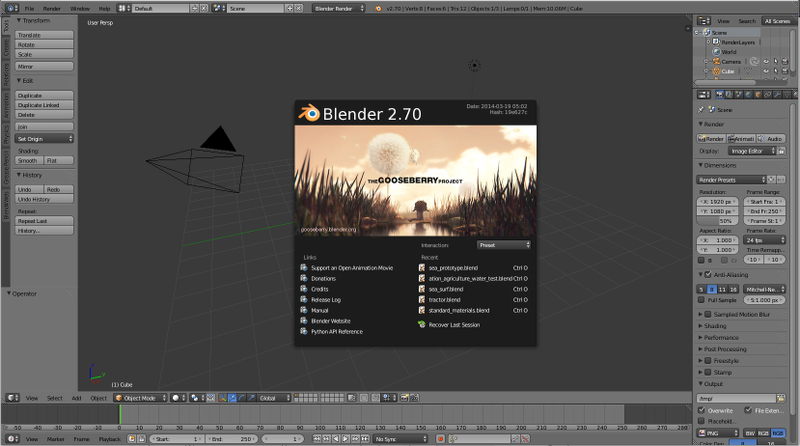
\includegraphics[width=1.000\linewidth]{blender_first_run.jpg}\hfill}

\index{export!Blender installation}

\section{The Engine Addon Install}
\label{first_steps:index-0}\label{first_steps:id4}\label{first_steps:first-step-addon}
Run Blender, load the default scene \code{File \textgreater{} New}. Show the user preferences \code{File \textgreater{} User Preferences...}. Under the \code{Addons} tab click \code{Install from File...} and then select the zip archive with the addon files. After that turn on the \code{Import-Export: Blend4Web}  checkbox.

{\hfill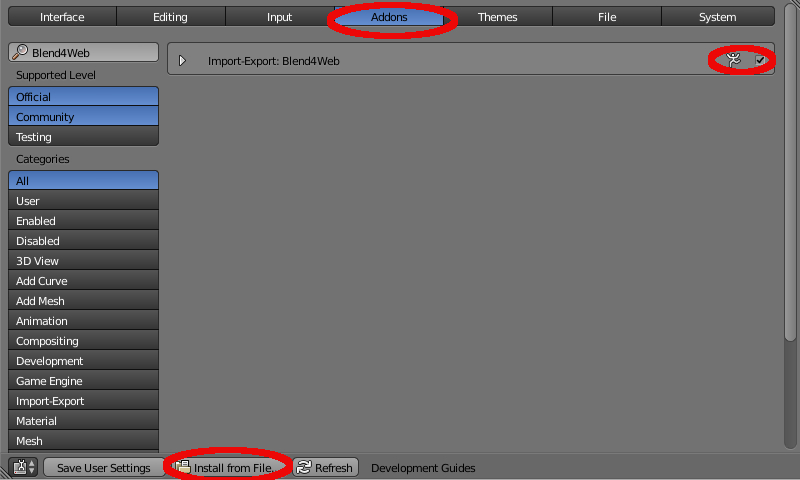
\includegraphics[width=1.000\linewidth]{user_preferences_install_b2w.jpg}\hfill}

Then click \code{Save User Settings} and close the user preferences window.

\index{export!addon installation}

\section{Exporting and Viewing Scenes}
\label{first_steps:first-step-export-view}\label{first_steps:id5}\label{first_steps:index-1}
The created scenes can be exported in HTML format. To do this use the \code{File \textgreater{} Export \textgreater{} Blend4Web (.html)} menu option and choose the export filepath. The resulting HTML file can be opened with any browser with WebGL support.


\strong{See also:}


{\hyperref[about:browser-webgl-support]{\emph{WebGL Browsers Support}}}



\index{export!viewing scenes}

\chapter{Development Environment Setup}
\label{setup:setup}\label{setup::doc}\label{setup:index-2}\label{setup:id1}
This setup option suits 3D application developers. To familiarize yourself with the Blend4Web addon {\hyperref[first_steps:first-steps]{\emph{quick install}}} can be a better option.

In order to work you must have the engine distribution, a browser (suitable for local viewing) and Blender (with the addon installed).


\section{Distribution Installation}
\label{setup:getting-started-distribution}\label{setup:id2}
Stable versions of the distribution are available as an archive (\code{blend4web\_sdk\_free.zip} -- free SDK, \code{blend4web\_sdk\_pro.zip} -- commercial SDK). Simply unpack this archive somewhere.

The distribution consists of the engine's source code, the minified version for applications, the Blender scripts, the source blend-files, the exported scenes, textures and sound files (see detailed {\hyperref[developers:repo-file-structure]{\emph{repository structure}}}).

\index{browser!setup}

\section{Browser Setup}
\label{setup:index-0}\label{setup:getting-started-browser}\label{setup:id3}
The engine requires a browser with WebGL support (for example, Chrome or Firefox). Just to check it open the page \href{http://get.webgl.org/}{http://get.webgl.org/}. The green message and rotating cube should appear:

{\hfill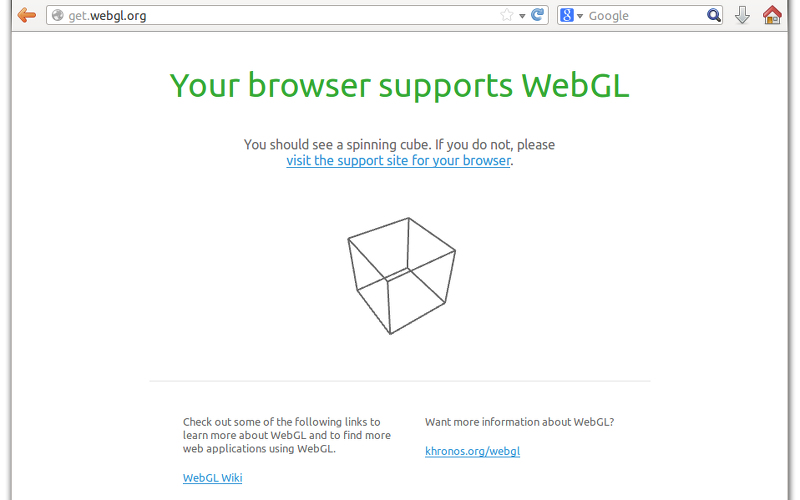
\includegraphics[width=1.000\linewidth]{browser_supports_webgl.jpg}\hfill}

\index{Blend4Web!installation}
A browser should be set up for loading resources from the local filesystem. To do this add the \code{-{-}allow-file-access-from-files} option to (e.g.) Chrome launcher (detailed info {\hyperref[problems_and_solutions:browser-for-local-loading]{\emph{about the setup}}}).

\index{viewer!launch}

\section{Running The Scenes Viewer}
\label{setup:id4}\label{setup:getting-started-launching-viewer}\label{setup:index-2}
Open the \code{apps\_dev/viewer/viewer\_dev.html} file in a set up browser. The page with the renderer window and interface elements should be displayed.

{\hfill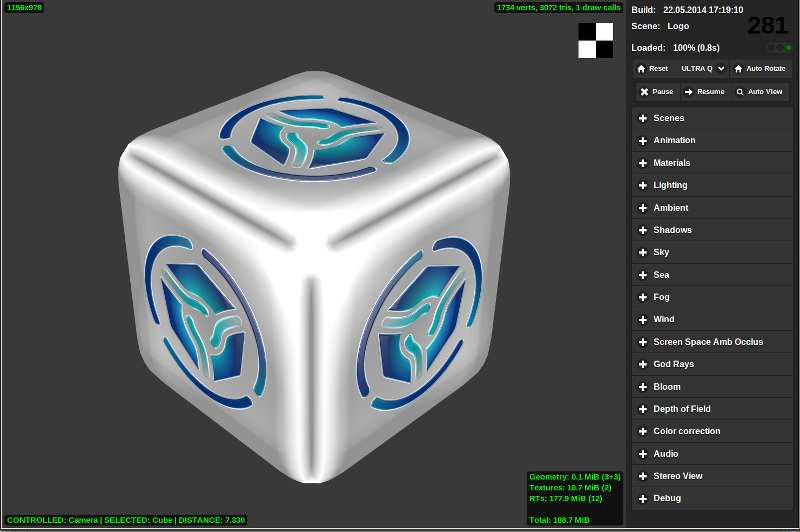
\includegraphics[width=1.000\linewidth]{default_page.jpg}\hfill}

\begin{DUlineblock}{0em}
\item[] 
\end{DUlineblock}

\begin{notice}{note}{Note:}
If the page isn't displayed correctly, or an error message is shown, follow the instructions described in the {\hyperref[problems_and_solutions:renderer-not-working]{\emph{Проблемы при запуске рендерера}}} section.
\end{notice}

\index{Blender!installation}

\section{Engine Addon Installation}
\label{setup:getting-started-addon}\label{setup:id5}\label{setup:index-3}
\begin{notice}{note}{Note:}
It is recommended to remove the addon first if it was originally installed using {\hyperref[first_steps:first-steps]{\emph{quick install}}}.
\end{notice}

Run Blender, load the default scene \code{File \textgreater{} New} (hot keys \code{Ctrl-N}). Open the user preferences window \code{File \textgreater{} User Preferences...} (hot keys \code{Ctrl-Alt-U}). Under the \code{File} tab in the \code{Scripts} field choose the path to the \code{blender\_scripts} directory.

{\hfill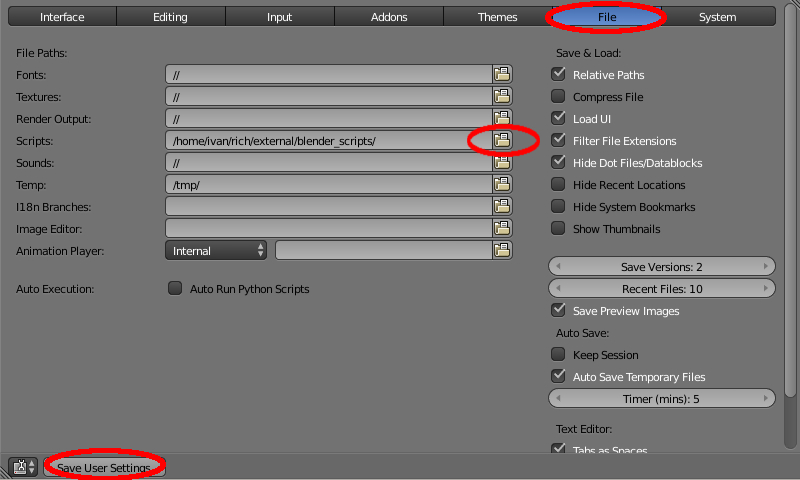
\includegraphics[width=1.000\linewidth]{user_preferences_scripts_path.jpg}\hfill}

Click \code{Save User Settings} and restart Blender.

\begin{notice}{note}{Note:}
Instead of this it's possible to copy the scripts directory \code{blender\_scripts/addons/blend4web} to the already used directory for scripts or even to the install directory, for example:

\code{C:\textbackslash{}Program Files\textbackslash{}Blender Foundation\textbackslash{}Blender\textbackslash{}2.70\textbackslash{}scripts\textbackslash{}addons\textbackslash{}blend4web}.
\end{notice}

Again load the default scene, open the user preferences window, go to the \code{Addons} tab and choose the \code{Import-Export} category. Enable the \code{Import-Export: Blend4Web} checkbox.

{\hfill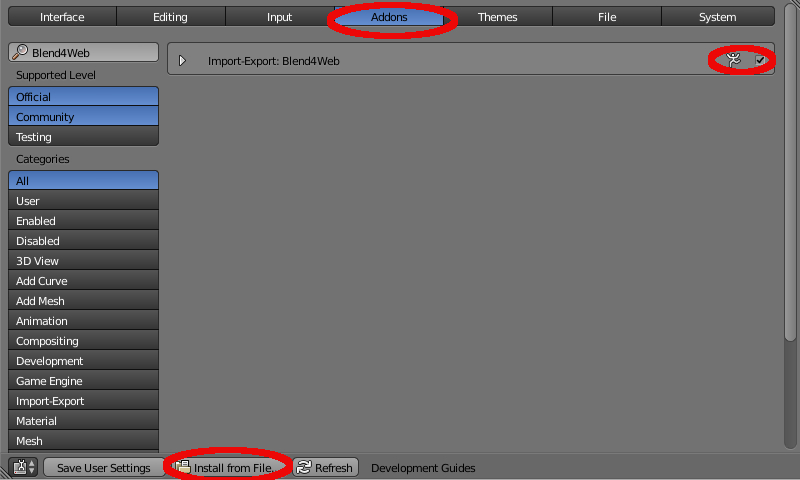
\includegraphics[width=1.000\linewidth]{user_preferences_enable_addon.jpg}\hfill}

Click \code{Save User Settings}. Restarting Blender isn't required.

\emph{To check:}

In the \code{File \textgreater{} Export} menu the \code{Blend4Web (.json)} and \code{Blend4Web (.html)} options should appear. Also the operators should appear in the search box when searching for ``B4W'' (hot key \code{SPACE}).


\subsection{Enabling the HTML export option}
\label{setup:html}
The \code{Blend4Web (.html)} option in the \code{File \textgreater{} Export} menu is not active by default contrary to the standalone version of the addon (see {\hyperref[first_steps:first-steps]{\emph{Quick Install}}}).

If required (for example for HTML export debugging) this option can be enabled. To do this specify the path to the \code{embed} application build of the distribution in the \code{Path to b4w source} field. The standard path relative to the engine's root is \code{external/deploy/apps/embed}.

{\hfill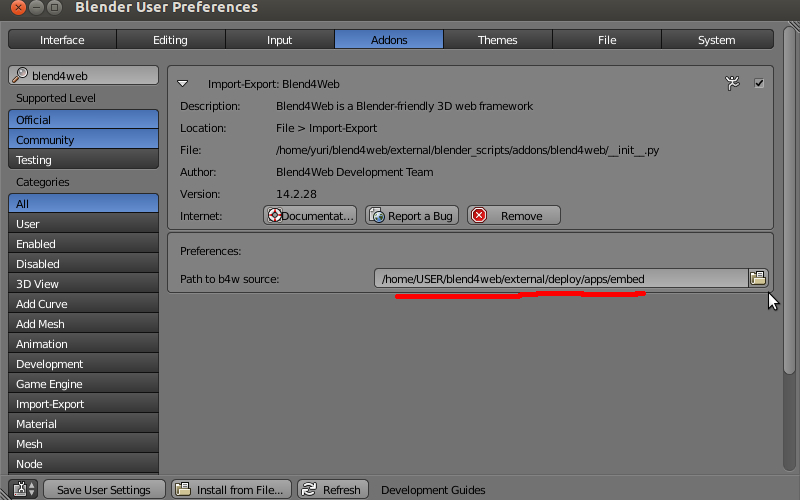
\includegraphics[width=1.000\linewidth]{user_preferences_enable_addon_HTML_option.jpg}\hfill}


\chapter{Workflow}
\label{workflow::doc}\label{workflow:working-process-stages}\label{workflow:id1}
Developing any product is a creative process with many participants who have different skills and experience. However no matter how complex it is and what is the target it's always possible to separate the production stage in which the bulk of assets and source code is authored.

When using Blend4Web the workflow is the following:
\begin{enumerate}
\item {} 
Preparing a 3D scene in Blender.

\item {} 
Exporting the resources in a format suitable for the engine.

\item {} 
Running, tweaking and debugging the scene in the viewer.

\item {} 
Creating the target application.

\end{enumerate}


\section{Preparing the Scenes}
\label{workflow:id2}
Besides the usual stages such as modeling, texturing, animation etc a scene should be prepared for working in the engine.

General recommendations:
\begin{enumerate}
\item {} 
Blend-files should be located in the \code{external/blender/project\_name} directory.

\item {} 
Texture and sound files should be external and located in the \code{external/deploy/assets/project\_name} directory.

\item {} 
Auxiliary files which are not intended for loading into the engine (for example, references), should be located in the \code{external/blender/project\_name} directory.

\item {} 
The file from which export will occur should only contain models required for the application being developed.

\item {} 
Object, mesh, material, texture, armature etc should have distinct names (in English). They should not be named ``Cube.001'', ``Material'', ``Armature''.

\item {} 
Its possible to link components from other (library) files.

\end{enumerate}

\index{export}

\section{Exporting Scenes}
\label{workflow:index-0}\label{workflow:id3}
In order to load scenes authored in Blender into the engine you have to transform them into the format suitable for reading by a browser. At the moment text files with \code{.json} extension are used in which exported data structures in JSON (JavaScript Object Notation) format are saved. This file, in turn, refers to one binary file with a \code{.bin} extension containing data arrays of models and to external resources - textures and sound samples.

While the \code{.json} and \code{.bin} files are created upon export, texture and sound files are normally placed by hand (there is an exception though: resources embeded into a \code{.blend}-file are placed automatically).

Export can be performed by choosing the \code{Blend4Web (.json)} option from the \code{File \textgreater{} Export} menu. Quick access - search for \code{b4w export} (hot key \code{SPACE}).

It is recommended to place files intended for export into the directory intended for application deploy, for example \code{external/deploy/assets/project\_name}.

It's necessary to use relative filepaths for images (normally this is by default). If this is not the case, execute the \code{File \textgreater{} External Data \textgreater{} Make All Paths Relative} operator. Using absolute filepaths instead of relative ones may lead to errors when loading \code{.blend} and \code{.json} files on other computers.

Upon export the scene is checked for Blender features not supported by the engine. In such cases an error message is generated:

{\hfill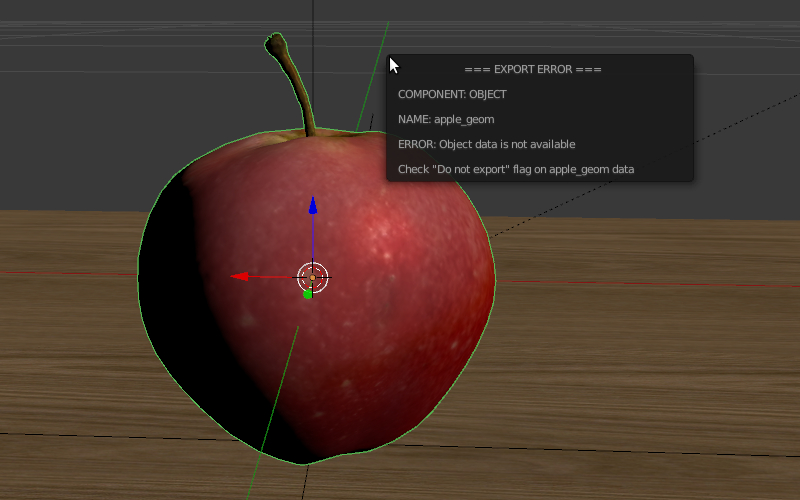
\includegraphics[width=1.000\linewidth]{error_message.jpg}\hfill}

\begin{DUlineblock}{0em}
\item[] 
\end{DUlineblock}

The list of possible export errors is specified in the {\hyperref[addon:export-errors]{\emph{corresponding section}}}.


\subsection{Export Options}
\label{workflow:id4}\begin{description}
\item[{\emph{Autosave main file}}] \leavevmode
Autosaving the file from which export occurs. \textbf{Is turned on by default}. This happens right after the export to guarantee conformity between the current blend-file and the exported file content. In addition, the relative path to the exporting file is saved for convenience.

\item[{\emph{Filepath}}] \leavevmode
Path to the export file. It is used in command-line export mode and not used in windowed mode.

\end{description}

\index{viewer!scene adding}

\section{Displaying Scenes in the Viewer}
\label{workflow:id5}\label{workflow:index-1}
For the scene to appear in the viewer list it's required to manually add an entry to the text file \code{external/deploy/assets/assets.js}.

For new scene adding it's needed to know the category in which a scene will be displayed. The category normally corresponds to the project name and to the name of the directory where corresponding files are stored.


\subsection{Example}
\label{workflow:id6}
Below an example part of \code{assets.js} file is given with two projects ``Capri'' and ``Fridge'' with the corresponding scenes in each project:

\begin{Verbatim}[commandchars=\\\{\}]
\PYG{p}{\PYGZob{}}
    \PYG{n}{name}\PYG{p}{:} \PYG{l+s}{\PYGZdq{}}\PYG{l+s}{Capri}\PYG{l+s}{\PYGZdq{}}\PYG{p}{,}
    \PYG{n}{items}\PYG{p}{:} \PYG{p}{[}
        \PYG{p}{\PYGZob{}}
            \PYG{n}{name}\PYG{p}{:} \PYG{l+s}{\PYGZdq{}}\PYG{l+s}{Baken}\PYG{l+s}{\PYGZdq{}}\PYG{p}{,}
            \PYG{n}{load\PYGZus{}file} \PYG{p}{:} \PYG{l+s}{\PYGZdq{}}\PYG{l+s}{capri/props/baken/baken.json}\PYG{l+s}{\PYGZdq{}}
        \PYG{p}{\PYGZcb{}}\PYG{p}{,}
        \PYG{p}{\PYGZob{}}
            \PYG{n}{name}\PYG{p}{:} \PYG{l+s}{\PYGZdq{}}\PYG{l+s}{Terrain}\PYG{l+s}{\PYGZdq{}}\PYG{p}{,}
            \PYG{n}{load\PYGZus{}file} \PYG{p}{:} \PYG{l+s}{\PYGZdq{}}\PYG{l+s}{capri/landscape/terrain/terrain.json}\PYG{l+s}{\PYGZdq{}}
        \PYG{p}{\PYGZcb{}}
    \PYG{p}{]}
\PYG{p}{\PYGZcb{}}\PYG{p}{,}
\PYG{p}{\PYGZob{}}
    \PYG{n}{name}\PYG{p}{:} \PYG{l+s}{\PYGZdq{}}\PYG{l+s}{Fridge}\PYG{l+s}{\PYGZdq{}}\PYG{p}{,}
    \PYG{n}{items}\PYG{p}{:} \PYG{p}{[}
        \PYG{p}{\PYGZob{}}
            \PYG{n}{name}\PYG{p}{:} \PYG{l+s}{\PYGZdq{}}\PYG{l+s}{Apple}\PYG{l+s}{\PYGZdq{}}\PYG{p}{,}
            \PYG{n}{load\PYGZus{}file} \PYG{p}{:} \PYG{l+s}{\PYGZdq{}}\PYG{l+s}{fridge/fruits/apple/apple.json}\PYG{l+s}{\PYGZdq{}}
        \PYG{p}{\PYGZcb{}}\PYG{p}{,}
        \PYG{p}{\PYGZob{}}
            \PYG{n}{name}\PYG{p}{:} \PYG{l+s}{\PYGZdq{}}\PYG{l+s}{Mango}\PYG{l+s}{\PYGZdq{}}\PYG{p}{,}
            \PYG{n}{load\PYGZus{}file} \PYG{p}{:} \PYG{l+s}{\PYGZdq{}}\PYG{l+s}{fridge/fruits/mango/mango.json}\PYG{l+s}{\PYGZdq{}}
        \PYG{p}{\PYGZcb{}}
    \PYG{p}{]}
\PYG{p}{\PYGZcb{}}
\end{Verbatim}

Adding may be performed by copying and pasting of a similar scene description in the required category and by further editing of its name and path to the exporting file.

In case of successful adding a scene should appear in the viewer scenes list in the required category.

{\hfill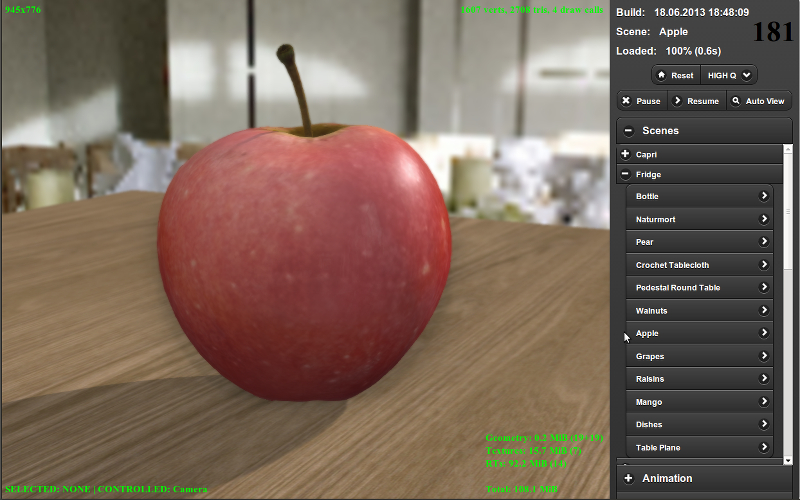
\includegraphics[width=1.000\linewidth]{viewer_apple_scene.jpg}\hfill}


\section{Application Development}
\label{workflow:id7}
On this stage an application is created and a logic for scene loading and user interaction is described using JavaScript language. The application developer notes are given in the {\hyperref[developers:developers]{\emph{corresponding section}}}.

\index{viewer}

\chapter{Scene Viewer}
\label{viewer:viewer}\label{viewer:index-0}\label{viewer::doc}\label{viewer:id1}
{\hyperref[setup:getting-started-launching-viewer]{\emph{Scene viewer run}}}.


\section{Navigation}
\label{viewer:id2}
Camera control is performed using mouse with a pressed button, as well as using \code{W}, \code{A}, \code{S}, \code{D}, \code{R}, \code{F} keys: forward, to the left, back, to the right, upward, downward. Also arrows and \code{numpad} keys can be used. In the \code{Target} camera mode it's possible to focus on the selected object by means of \code{Z} or \code{.(dot)} keys.


\section{The Side Panel}
\label{viewer:id3}
The side panel contains three areas: the information board, basic control buttons and the list of drop-down panels with additional control elements differentiated by functionality.

{\hfill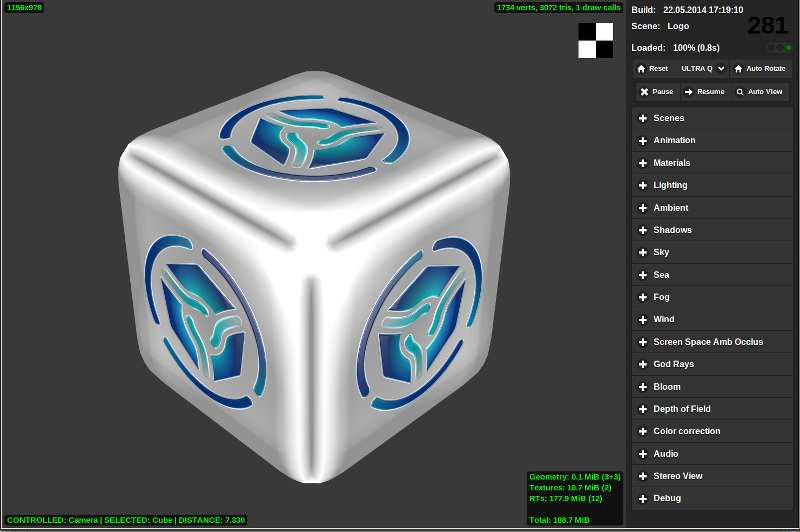
\includegraphics[width=1.000\linewidth]{default_page.jpg}\hfill}

\begin{DUlineblock}{0em}
\item[] 
\end{DUlineblock}


\subsection{Control elements list in top-down order}
\label{viewer:id4}\begin{description}
\item[{\textbf{Build}}] \leavevmode
The engine build date and time. In developer version this shows page load time.

\item[{\textbf{Scene}}] \leavevmode
Loaded scene name from the \code{assets.js} file. Path to the file pops-up on mouse hover.

\item[{\textbf{Loaded}}] \leavevmode
Loading progress and time.

\item[{\textbf{Reset}}] \leavevmode
This button deletes the saved name of the last viewed scene and reloads the page back to display the default scene.

\item[{\textbf{LOW Q - HIGH Q - ULTRA Q}}] \leavevmode
Drop-down menu for choosing the performance profile of the engine:
\begin{itemize}
\item {} 
\emph{low quality} - a range of functions is turned off (such as postprocessing), size of textures is halved when using a release version, anti-aliasing is turned off

\item {} 
\emph{high quality} - all requested by scene features are used, anti-aliasing method is FXAA

\item {} 
\emph{maximum quality} - rendering resolution is doubled, anti-aliasing method is SMAA

\end{itemize}

\item[{\textbf{Pause}}] \leavevmode
Pause rendering.

\item[{\textbf{Resume}}] \leavevmode
Resume rendering.

\item[{\textbf{Auto View}}] \leavevmode
Activation of automatic scene switching mode; the pause between views is 1 second.

\item[{\textbf{Scenes}}] \leavevmode
The two-level list of the categories and scenes from the \code{assets.json} file.

\item[{\textbf{Animation}}] \leavevmode
Animation controls. When viewing animated model it's possible to select an object and switch animation for it using drop-down menu, switch cyclic animation mode, stop and resume animation, set the required frame (to do this the animation should be stopped).

\item[{\textbf{Materials}}] \leavevmode
Material properties setup. A material can be selected using the drop-down menu. At the moment only limited range of properties is supported.

\item[{\textbf{Lighting}}] \leavevmode
Direct lighting parameters setup. A light source can be selected using the drop-down menu. Changing color and intensity is supported. Also on this panel day time and sun lighting parameters can be tweaked.

\item[{\textbf{Ambient}}] \leavevmode
Ambient lighting parameters setup. Changing colors of hemispheric ambient model and intensity is supported.

\item[{\textbf{Shadows}}] \leavevmode
Shadow parameters setup, including parameters of shadow cascades and parameters of shadow edges softening.

\item[{\textbf{Sky}}] \leavevmode
Dynamic sky parameters setup such as color, sun light scattering parameters etc.

\item[{\textbf{Sea}}] \leavevmode
Water rendering parameters setup, including color transitions by depth and by shore distance, foam and subsurface scattering parameters, waves dynamics etc.

\item[{\textbf{Fog}}] \leavevmode
Fog parameters setup, including density and color.

\item[{\textbf{Wind}}] \leavevmode
Wind parameters setup, including direction and strength.

\item[{\textbf{Screen Space Amb Occlus}}] \leavevmode
Ambient occlusion parameters setup.

\item[{\textbf{God Rays}}] \leavevmode
Crepuscular rays effect parameters setup.

\item[{\textbf{Bloom}}] \leavevmode
Bright light effect parameters setup.

\item[{\textbf{Depth of Field}}] \leavevmode
Depth of field effect parameters setup.

\item[{\textbf{Color correction}}] \leavevmode
Color correction parameters setup, including brightness, contrast, exposure and saturation.

\item[{\textbf{Anti-aliasing}}] \leavevmode
Selection of anti-aliasing method.

\item[{\textbf{Audio}}] \leavevmode
Mixing mode switch is located on this panel. After switching it on the mixer interface becomes visible (only for scenes with sound sources).

\item[{\textbf{Stereo View}}] \leavevmode
Stereoscopy mode switch is located on this panel.

\item[{\textbf{Debug}}] \leavevmode
A range of debugging tools is located on this panel, particularly wireframe mode switch, switch for postprocessing stages viewer.

\end{description}


\section{Indicators}
\label{viewer:id5}\begin{description}
\item[{\textbf{Frames per second counter}}] \leavevmode
This is located in the right top corner. It displays the averaged and rounded value for last 1.5 seconds.

\item[{\textbf{Viewport dimensions}}] \leavevmode
This is located in the left top corner. It displays the viewport dimensions in pixels.

\item[{\textbf{Selected object and controlled object}}] \leavevmode
This is located in the left bottom corner. It displays selected and controlled objects names. Object selection can be performed using mouse. For getting the direct control over the object (normally for physics debugging) it's needed to press \code{Q} key and click on the object. Object movement is performed using \code{W}, \code{A}, \code{S}, \code{D} keys. To exit the control mode press the \code{Q} key and click on empty space. The indicator also displays the distance to the selected object in Blender units (meters equivalent).

\item[{\textbf{Scene complexity indicator}}] \leavevmode
This is located in the right top relative to the rendering area. It displays the number of vertices, triangles and WebGL calls on the main rendering scene (i.e. shadow rendering calls are not included, for example).

\item[{\textbf{Video memory indicator}}] \leavevmode
This is located in the right bottom relative to the rendering area. It displays video memory amount used by geometry, textures, render targets, and also the total memory usage.

\end{description}

{\hfill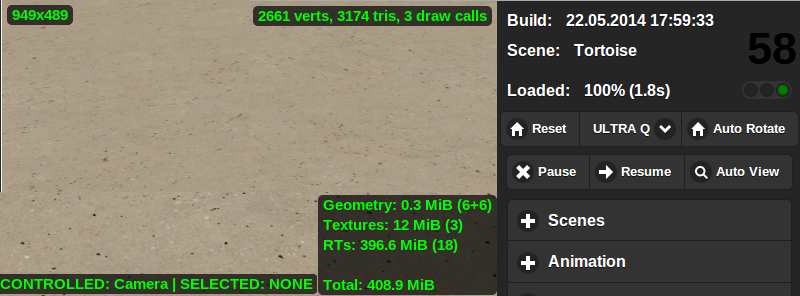
\includegraphics[width=1.000\linewidth]{indicators.jpg}\hfill}


\chapter{The Addon}
\label{addon:id1}\label{addon::doc}\label{addon:addon}
\index{initialization!compatibility!errors}

\section{Initialization Errors}
\label{addon:id2}\label{addon:index-0}\label{addon:initialization-errors}
Initialization errors can arise upon install of the addon or when a scene is opened in Blender. In this case a dialog window with the error description is showed.

{\hfill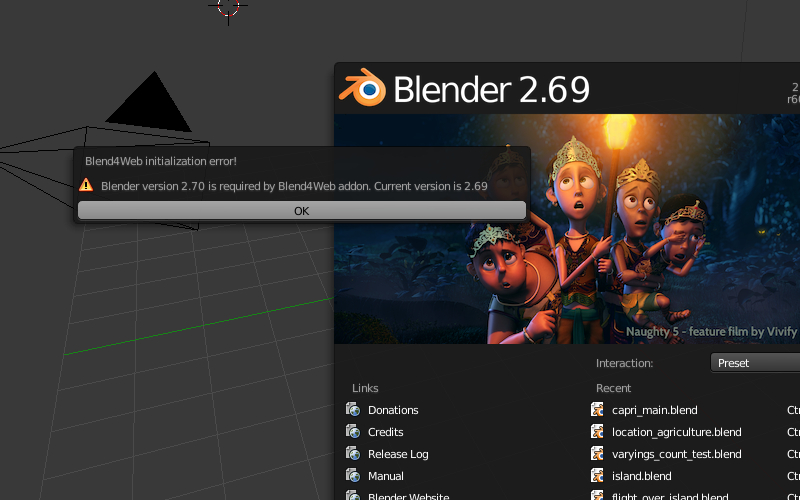
\includegraphics[width=1.000\linewidth]{init_error_message.jpg}\hfill}

\begin{DUlineblock}{0em}
\item[] 
\end{DUlineblock}

\begin{tabulary}{\linewidth}{|L|L|}
\hline
\textsf{\relax 
Error description
} & \textsf{\relax 
Cause
}\\
\hline
Blend4Web initialization error!
Addon is not compatible with
PLATFORM platform.
 & 
The Blend4Web addon is not compatible with the PLATFORM platform.
\\

Blend4Web initialization error!
Blender version VER\_REQUIRED is
required by Blend4Web addon.
Current version is VER\_CURRENT.
 & 
The Blend4Web addon is not compatible with Blender version used.
\\
\hline\end{tabulary}


\index{export!errors}

\section{Export Errors}
\label{addon:export-errors}\label{addon:index-1}\label{addon:id3}
Dialog window \code{BLEND4WEB EXPORT ERROR} with the problem description appears when export errors happen:
\begin{quote}

\code{COMPONENT} - type of component (object, mesh, material, texture etc) that caused export error.

\code{NAME} - component name.

\code{ERROR} - short description of the occured problem.
\end{quote}

{\hfill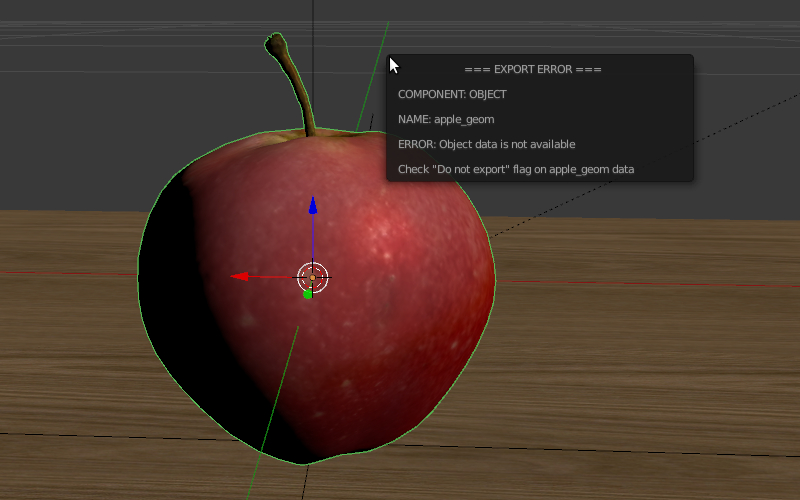
\includegraphics[width=1.000\linewidth]{error_message.jpg}\hfill}

\begin{DUlineblock}{0em}
\item[] 
\end{DUlineblock}

\begin{tabulary}{\linewidth}{|L|L|}
\hline
\textsf{\relax 
Error description
} & \textsf{\relax 
Cause
}\\
\hline
Dupli group error; Objects from
dupli group GROUP\_NAME on object
OBJECT\_NAME don't export
 & 
None of the objects in the GROUP\_NAME group which was selected for duplication on the OBJECT\_NAME object does export. It's required to permit the export of at least one object of the group, or to remove the duplication of the group.
\\

Incompatible meshes; Check
MESH\_NAME1 and MESH\_NAME2 UV Maps/
Vertex colors
 & 
There are two meshes with the same material. Such meshes are merged automatically into one by the engine with the purpose of optimization, and so they should have the same number of \code{UV Maps} and \code{Vertex Colors}.
\\

Incompatible objects with
shared mesh; Object OBJECT\_NAME
has vertex groups and shared mesh
 & 
Export of an object with the shared mesh and with vertex groups is not allowed. Exceptions: export is possible if an object has turned on options \code{Apply modifiers}, \code{Export vertex animation}, \code{Export edited normals} (because in these cases full copying of meshes occurs).
\\

Incomplete mesh; Dynamic grass
vertex colors required
by material settings
 & 
Special material for terrain uses options \code{Dynamic grass size} and/or \code{Dynamic grass color} but the mesh has no vertex colors with such names.
\\

Incomplete mesh; Material slot is
empty
 & 
Material slot is empty.
\\

Incomplete mesh; No UV in mesh
with UV-textured material
 & 
In the material of the mesh there are textures with texture coordinates type \code{UV}, but the mesh lacks UV map layers.
\\

Incomplete mesh; Vertex colors
required by material settings
 & 
The material of the mesh has turned on checkbox \code{Vertex Color Paint}, but the mesh lacks vertex colors.
\\

Incomplete vehicle. Vehicle NAME
hasn't chassis or hull.
 & 
The modelled vehicle named NAME is not complete as it should contain a \code{Chassis} or a \code{Hull} element.
\\

Incomplete vehicle. Vehicle NAME
requires at least one bob.
 & 
The modelled vehicle named NAME is not complete as it should contain at least one \code{Bob} element.
\\

Incomplete vehicle. Vehicle NAME
requires at least one wheel.
 & 
The modelled vehicle named NAME is not complete as it should contain at least one \code{Wheel} element.
\\
\hline\end{tabulary}


\begin{tabulary}{\linewidth}{|L|L|}
\hline

Incorrect mesh; Wrong group indices
 & 
The mesh has vertices assigned to the non-existing vertex group.
\\

Incorrect vertex animation; Object
has no any vertex animation
 & 
For the mesh the checkbox for exporting vertex animation is turned on, but there is no vertex animation.
\\

Incorrect vertex animation; Unbaked
vertex animation ``ANIM\_NAME''
 & 
Vertex animation export is turned on for the mesh, but the ANIM\_NAME animation has not a single frame.
\\

Material has normalmap but doesn't
have material node
 & 
The node material uses \code{Normal Mapping}, but has no \code{Material} node.
\\

Mesh has UV map but lacks any
exported material
 & 
The mesh has a UV map layer but has not any exporting material.
\\

Mesh has vertex color layer but
lacks any exported material
 & 
The mesh has a vertex color layer but has not any exporting material.
\\

Missing active camera
 & 
There is no active camera on the scene (property \code{Camera} on the \code{Scene} tab).
\\

Missing lamp
 & 
The scene should have at least one light source.
\\

Missing world
 & 
The scene should have at least one world datablock.
\\

No image
 & 
The texture lacks an image.
\\

No such file or directory
 & 
The file or directory does not exist.
\\

No texture in texture slot
 & 
There is no a texture in the material texture slot.
\\

Node material is invalid; Check
sockets compatibility: FROM\_NODE to
TO\_NODE
 & 
Node material error: input and output types of the link between nodes \code{FROM\_NODE} and \code{TO\_NODE} should match.
\\

Object constraint has no target
 & 
For the object constraint (on the \code{Object Constraints} tab) the property \code{Target Object} was not set.
\\

Object data is not available;
Check ``Do not export'' flag
on OBJECT\_NAME data
 & 
The data for the object are not available. This error appears particulary when for the exporting object the \code{Do not export} property in the \code{Object Data} tab is set.
\\

Object-parent relation is not
supported; Clear parent inverse
transform
 & 
When using parenting it's required to reset transform for the child object using operator \code{Object \textgreater{} Parent \textgreater{} Clear Parent Inverse} (Alt-P).
\\
\hline\end{tabulary}


\begin{tabulary}{\linewidth}{|L|L|}
\hline

Only 2 UV textures are allowed for
mesh; Mesh has N UVs
 & 
The engine supports up to 2 UV texture layers in a mesh. The mesh has N number of UV texture layers.
\\

Particle system error; Dupli group
isn't specified
 & 
Particle system error: a group for the particle is not selected.
\\

Particle system error; Dupli object
isn't specified
 & 
Particle system error: an object for the particle is not selected.
\\

Particle system error; Dupli object
OBJECT\_NAME doesn't export
 & 
The OBJECT\_NAME object which is selected for the particle is not exported (it has \code{Do not export} checkbox set).
\\

Particle system error; No one valid
object exports from dupli group
GROUP\_NAME
 & 
No one of the objects in the GROUP\_NAME group which is selected for the particle is exported. Either such objects have \code{Do not export} checkbox set or the objects have unsuitable type. Supported object types: \code{MESH}.
\\

Particle system error; Vertex color
``NAME''(from\_name) missing in object
OBJECT\_NAME
 & 
The NAME vertex color is specified in the \code{from} field but it is lacking in the OBJECT\_NAME emitter.
\\

Particle system error; Vertex color
``NAME''(to\_name) missing in object
``OBJECT\_NAME'' in dupli group
``GROUP\_NAME''
 & 
The NAME vertex color is specified in the \code{to} field but it is lacking in the OBJECT\_NAME object of the GROUP\_NAME group which is selected for the particle.
\\

Particle system error; Vertex color
``NAME''(to\_name) missing in object
OBJECT\_NAME
 & 
The NAME vertex color is specified in the \code{to} field but it is lacking in the OBJECT\_NAME object which is selected for the particle.
\\

Particle system error; Wrong dupli
object type TYPE\_NAME
 & 
The object of unsuitable type is selected for the particle. Supported types: \code{MESH}.
\\

Permission denied
 & 
No access to the current directory.
\\

Wind bending: vertex colors weren't
properly assigned
 & 
Wind bending parameters setup: it's required to specify names of either all vertex color layers (\code{Main stiffness (A)}, \code{Leaves stiffness (R)}, \code{Leaves phase (G)}, \code{Overall stiffness (B)}), or of the main one only (\code{Main stiffness (A)}), or of none of them.
\\

Wind bending: not all
vertex colors exist
 & 
Wind bending parameters setup: all specified vertex color layers should exist.
\\
\hline\end{tabulary}


\begin{tabulary}{\linewidth}{|L|L|}
\hline

Wrong edited normals count; It
doesn't match with mesh vertices
count
 & 
Number of edited normals do not match the number of mesh vertices. It's required to execute \code{Clean Up} or \code{Save} in the \code{B4W Vertex Normals Editor} panel.
\\

Wrong overrided bounding box; Check
mesh's bounding box values
 & 
Wrong dimensions are specified when overriding the mesh's \code{BoundingBox}: minimum value is greater than maximum value for at least one of dimensions.
\\

Wrong texture coordinates type
 & 
For textures with images the following coordinate types are supported: \code{UV}, \code{Normal}.
\\

Wrong vertex animation vertices
count; It doesn't match with mesh
vertices count for ``ANIM\_NAME''
 & 
Vertex animation export is turned on but the number of vertices in the baked ANIM\_NAME animation frames does not match the mesh vertices number. Possible solution is to ``re-bake'' the animation.
\\
\hline\end{tabulary}



\chapter{Objects}
\label{objects:objects}\label{objects::doc}\label{objects:id1}
Objects are intended for positioning of components of different types (meshes, cameras, lamps etc) in a 3D scene space.


\section{Types}
\label{objects:id2}
The engine supports objects of the following types:
\begin{itemize}
\item {} 
mesh

\item {} 
camera

\item {} 
lamp

\item {} 
empty

\item {} 
curve

\item {} 
armature

\item {} 
speaker

\item {} 
force field

\end{itemize}


\section{Settings}
\label{objects:id3}
For objects of all types it's supported the following: transform, reference to data, parent object, group membership and a range of the engine special properties.
\begin{figure}[htbp]
\centering

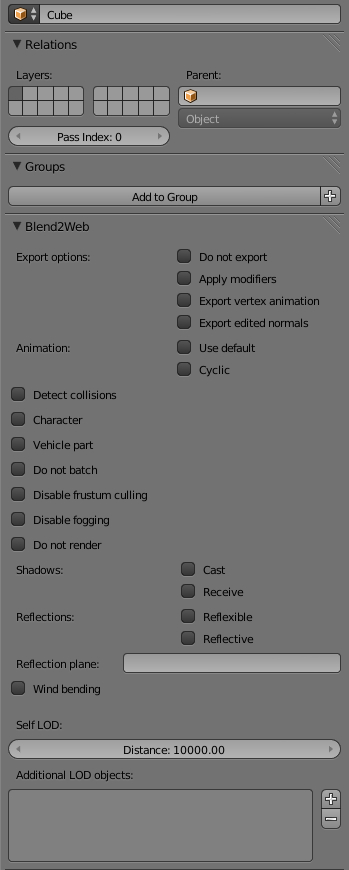
\includegraphics[width=0.600\linewidth]{object_setup.jpg}
\end{figure}
\begin{description}
\item[{\emph{Transform \textgreater{} Location}}] \leavevmode
Position coordinates.

\item[{\emph{Transform \textgreater{} Rotation}}] \leavevmode
Rotation angles. Shoud be used \code{XYZ Euler} mode which is set by default.

\item[{\emph{Transform \textgreater{} Scale}}] \leavevmode
Scaling. All 3 components (x, y, z) should be the same. Scaling for the physics objects is not supported.

\item[{\emph{Object Data} (tab)}] \leavevmode
Reference to the datablock which is specific for the objects of different types.

\item[{\emph{Relation \textgreater{} Parent}}] \leavevmode
Reference to the parent object.

\item[{\emph{Blend4Web \textgreater{} Do not export}}] \leavevmode
Do not export.

\item[{\emph{Blend4Web \textgreater{} Apply modifiers}}] \leavevmode
Apply the object's modifiers upon export.

\item[{\emph{Blend4Web \textgreater{} Export vertex animation}}] \leavevmode
Export previously created and saved vertex animation.

\item[{\emph{Blend4Web \textgreater{} Export edited normals}}] \leavevmode
Export previously edited and saved normals.

\item[{\emph{Blend4Web \textgreater{} Animation \textgreater{} Use default}}] \leavevmode
Upon loading into the engine start playback of the animation assigned to the object.

\item[{\emph{Blend4Web \textgreater{} Animation \textgreater{} Cyclic}}] \leavevmode
Сyclically repeat the animation assigned to the object. Animation cycling is also applied to particle systems ands speakers (if they present)

\item[{\emph{Blend4Web \textgreater{} Detect collisions}}] \leavevmode
Activate object physics.

\item[{\emph{Blend4Web \textgreater{} Character}}] \leavevmode
Enable the object usage as a physics character.

\item[{\emph{Blend4Web \textgreater{} Vehicle part}}] \leavevmode
Enable the object usage as a physics vehicle part.

\item[{\emph{Blend4Web \textgreater{} Do not batch}}] \leavevmode
Prohibit merging of object's mesh with other meshes with the same material which is performed by default for optimization purposes. Objects having animation or physics are already considered as separate. This option shoud be used in cases when the object movement is required but it's not apparent from its settings.

\item[{\emph{Blend4Web \textgreater{} Disable frustum culling}}] \leavevmode
Disable frustum culling optimization.

\item[{\emph{Blend4Web \textgreater{} Disable fogging}}] \leavevmode
Disable fog for the object.

\item[{\emph{Blend4Web \textgreater{} Do not render}}] \leavevmode
Disable object rendering (useful for a physics object for example).

\item[{\emph{Blend4Web \textgreater{} Shadows: Cast} и \emph{Blend4Web \textgreater{} Shadows: Receive}}] \leavevmode
Cast and receive shadows respectively. Can be turned on simultaneously.

\item[{\emph{Blend4Web \textgreater{} Reflections: Reflexible}}] \leavevmode
When enabled the object is reflected from the dynamic mirror surfaces.

\item[{\emph{Blend4Web \textgreater{} Reflections: Reflective}}] \leavevmode
When enabled the object surface reflexes other objects.

\item[{\emph{Blend4Web \textgreater{} Reflections: Reflection plane}}] \leavevmode
Text field for the name of the empty object defining the reflection plane.

\item[{\emph{Blend4Web \textgreater{} Wind bending}}] \leavevmode
Enable procedural animation under the influence of wind.

\item[{\emph{Blend4Web \textgreater{} Self LOD \textgreater{} Distance}}] \leavevmode
Distance from a camera on which the object no longer is rendered.

\item[{\emph{Blend4Web \textgreater{} Additional LOD objects}}] \leavevmode
Interface for adding low-poly objects used for switching levels of detail.

\end{description}


\section{Camera}
\label{objects:id4}
Camera settings are specified on the \code{Properties} panel in the \code{Object Data} tab.

\emph{Blend4Web \textgreater{} Move style} -- camera control mode. By default camera is in \code{Static} mode and this can be changed only through API call. In the \code{Target} mode the camera is rotating around the fixed point. The \code{Eye} mode allows rotation and translation as in first person view.

\emph{Blend4Web \textgreater{} Target location} -- available in the \code{Target} mode. This is position of the camera pivot point. The \code{Copy Cursor Location} buttons copies the current 3D cursor position into this value.

\emph{Blend4Web \textgreater{} Use distance limits} -- available in the \code{Target} mode. This limits camera transition by the two limiting distances.

\emph{Blend4Web \textgreater{} Use vertical rotation clamping} -- available in the \code{Target} and \code{Eye} modes. This limits vertical rotation angle of the camera by the two limiting values.

\emph{Blend4Web \textgreater{} DOF front distance} -- described in the {\hyperref[postprocessing_effects:postprocessing-effects]{\emph{Postprocessing effects}}} section.

\emph{Blend4Web \textgreater{} DOF rear distance} -- described in the {\hyperref[postprocessing_effects:postprocessing-effects]{\emph{Postprocessing effects}}} section.

\emph{Blend4Web \textgreater{} DOF power} -- described in the {\hyperref[postprocessing_effects:postprocessing-effects]{\emph{Postprocessing effects}}} section.
\phantomsection\label{textures:textures}
\index{textures}

\chapter{Textures}
\label{textures:index-0}\label{textures::doc}\label{textures:id1}
\index{textures!types}

\section{Texture types}
\label{textures:id2}\label{textures:index-1}
The drop-down menu \code{Type} for selecting texture type is located in the \code{Textures} tab. The engine supports the following texture types:
\begin{enumerate}
\item {} \begin{description}
\item[{\code{Image or Movie}}] \leavevmode\begin{itemize}
\item {} 
diffuse map

\item {} 
specular map, this also can be packed into the alpha channel of a diffuse texture

\item {} 
normal map

\item {} 
height map; this must be packed into the alpha channel of a normal map; it is used for relief surfaces visualization (parallax mapping).

\item {} 
transparency map (alpha map) - is used separately only for water rendering in the low quality mode; in a generic material this is contained in the alpha channel of a diffuse texture

\item {} 
stencil map

\end{itemize}

\end{description}

\item {} \begin{description}
\item[{\code{Environment Map}}] \leavevmode\begin{itemize}
\item {} 
mirror map

\item {} 
{\hyperref[textures:skydome-texture]{\emph{skydome texture}}}

\end{itemize}

\end{description}

\item {} \begin{description}
\item[{\code{None}}] \leavevmode\begin{itemize}
\item {} 
applied to the Blender's default scene cube, in the engine a gray texture is generated. Also it is used for {\hyperref[textures:render-to-texture]{\emph{rendering scene to texture}}}.

\end{itemize}

\end{description}

\item {} \begin{description}
\item[{\code{Blend}, gradient}] \leavevmode\begin{itemize}
\item {} 
is used in {\hyperref[particles:particles-textures]{\emph{particle systems}}}

\end{itemize}

\end{description}

\item {} \begin{description}
\item[{\code{Voronoi} procedural texture type}] \leavevmode\begin{itemize}
\item {} 
is used for water rendering to setup the caustics effect

\end{itemize}

\end{description}

\end{enumerate}

\index{textures!settings}

\section{Generic Settings}
\label{textures:id3}\label{textures:index-2}\begin{description}
\item[{\emph{Dimensions}}] \leavevmode
Bitmap dimensions for image textures (image width and height in pixels) should be a 2$^{\text{N}}$ number, i.e. 4, 8, 16, 32, 64, 128, 256, 512, 1024, 2048, 4096 px. Using textures with other dimensions (so-called NPOT) is supported but is not recommended. Dimensions should be at least 4 pixels for the correct texture compression. Normally square images are used (e.g. 512 x 512 px), however rectangular ones can be used too (e.g. 4 x 128 px). Using images bigger than 2048 px is not recommended.

\item[{\emph{Image Mapping \textgreater{} Extension}}] \leavevmode
Texture coordinates interpretation mode (Wrap Mode in WebGL). This is available for \code{Image or Movie} texture type. In case of \code{Repeat} value the engine sets the \code{REPEAT} mode for the texture. In this case the integer part of texture coordinates is ignored and a fractional part is used. In all other cases (for example \code{Extend}) the engine sets the \code{CLAMP\_TO\_EDGE} mode. In this case texture coordinates are limited by the {[}0, 1{]} segment. The default value is \code{Repeat}.

\end{description}

\index{material capture}\index{matcap}\begin{description}
\item[{\emph{Mapping \textgreater{} Coordinates}}] \leavevmode
Texture coordinates type. Supported types are \code{UV} (use UV map), \code{Normal} (use direction to the camera; available only for diffuse maps; used for creation of \textbf{material capture}, \textbf{matcap}). The default value is \code{Generated} (!).

\item[{\emph{Mapping \textgreater{} Offset}}] \leavevmode
Unsupported.

\item[{\emph{Mapping \textgreater{} Size}}] \leavevmode
Scaling of UV map by the respective axes. The default values are 1.0.

\item[{\emph{Blend4Web \textgreater{} Do not export}}] \leavevmode
Do not export the texture. Disabled by default.

\item[{\emph{Blend4Web \textgreater{} Anisotropic Filtering}}] \leavevmode
Anisotropic filtering factor for the individual texture. It has priority over the similar setting for the scene. The default value is \code{DEFAULT} (i.e. use the scene settings).

\item[{\emph{Blend4Web \textgreater{} UV translation velocity}}] \leavevmode
Animation speed of texture coordinates by the respective axes. The default values are 0.0.

\item[{\emph{Blend4Web \textgreater{} Water Foam}}] \leavevmode
The foam texture is used by the material for water rendering.

\end{description}

\index{textures!diffuse}\index{diffuse map}

\section{Diffuse map}
\label{textures:index-4}\label{textures:diffuse-map}
A diffuse map is used for specifying scattered light distribution (the Lambert model).


\subsection{Activation}
\label{textures:id4}
Set the \code{Diffuse \textgreater{} Color} checkbox on the \code{Textures \textgreater{} Influence} panel.


\subsection{Additional settings}
\label{textures:id5}\begin{description}
\item[{\emph{Influence \textgreater{} Diffuse \textgreater{} Color}}] \leavevmode
Influence of the texture on diffuse color. The default value is 1.0.

\item[{\emph{Influence \textgreater{} Blend}}] \leavevmode
The type of the interaction with the material color (\code{Material \textgreater{} Diffuse \textgreater{} Color}), or with the vertex color if the \code{Vertex Color Paint} checkbox is set. The following types are supported: \code{Mix} (mixes with the color), \code{Multiply} (multiplies by the color). The default value is \code{Mix}.

\end{description}

\index{textures!specular map}\index{specular map}

\section{Specular map}
\label{textures:index-5}\label{textures:specular-map}
The specular map is used for specifying of the reflected light color distribution (the Phong model).


\subsection{Activation}
\label{textures:id6}
Set the \code{Specular \textgreater{} Color} checkbox on the \code{Textures \textgreater{} Influence} panel (the \code{Specular \textgreater{} Intensity} checkbox is not supported).


\subsection{Additional settings}
\label{textures:id7}\begin{description}
\item[{\emph{Influence \textgreater{} Specular \textgreater{} Color}}] \leavevmode
The influence of the texture on the reflected light color. The default value is 1.0.

\item[{\emph{Influence \textgreater{} Blend}}] \leavevmode
The type of interaction with the reflected light color of the material (\code{Material \textgreater{} Specular \textgreater{} Color}). \code{Mix} (mixes with the color) is the only supported type. The default value is \code{Mix}.

\end{description}

The specular map can be packed to the alpha channel of a diffuse texture for optimization purposes. In such case it is required for the texture to set the \code{Diffuse \textgreater{} Color} and \code{Specular \textgreater{} Color} checkboxes simultaneously. The color range is limited by gray tints.

\index{textures!normal map}\index{normal map}

\section{Normal map}
\label{textures:index-6}\label{textures:normal-map}
A normal map is used for specifying distribution of surface normals (perpendiculars) with the purpose of its relief detalization. Normals information should be stored in the texture coordinate space. Normal maps in the object coordinate space are not supported.


\subsection{Activation}
\label{textures:id8}
Set the \code{Geometry \textgreater{} Normal} checkbox on the \code{Textures \textgreater{} Influence} panel.


\subsection{Additional settings}
\label{textures:id9}\begin{description}
\item[{\emph{Influence \textgreater{} Geometry \textgreater{} Normal}}] \leavevmode
Normal map influence on the resulting normals calculation. The default value is 1.0.

\end{description}

\index{textures!height map}\index{height map}\index{parallax mapping}

\section{Height map. Parallax mapping}
\label{textures:index-7}\label{textures:height-map-parallax-mapping}
A height map contains the information about distribution of relative relief heights. The higher the surface level the brighter its color. A height map in combination with a normal map is required for the implemetation of relief surface effect (parallax mapping). A height map should be contained in the alpha channel of a normal map.


\subsection{Activation}
\label{textures:id10}
Set the \code{Parallax} checkbox on the \code{Textures \textgreater{} Blend4Web} panel for a normal map in addition to the \code{Geometry \textgreater{} Normal} checkbox on the \code{Textures \textgreater{} Influence} panel.


\subsection{Additional settings}
\label{textures:id11}\begin{description}
\item[{\emph{Blend4Web \textgreater{} Parallax Scale}}] \leavevmode
Influence factor for relief surface effect. The default value is 0.03.

\item[{\emph{Blend4Web \textgreater{} Parallax Steps}}] \leavevmode
The number of iterations for the relief surface calculations. Bigger value leads to better quality but is more computationaly expensive.

\end{description}

{\hfill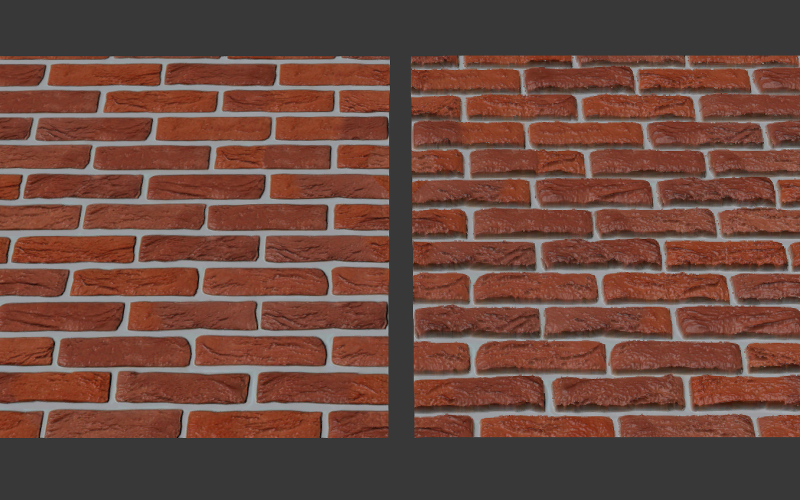
\includegraphics[width=1.000\linewidth]{parallax.jpg}\hfill}

\begin{DUlineblock}{0em}
\item[] 
\end{DUlineblock}

\index{textures!alpha map}\index{alpha map}

\section{Alpha map}
\label{textures:alpha-map}\label{textures:texture-alpha-map}\label{textures:index-8}
The separate alpha map is used only for low quality water rendering. In a generic material it can be contained in the alpha channel of a diffuse texture.


\subsection{Activation}
\label{textures:id12}
Set the \code{Diffuse \textgreater{} Alpha} checkbox on the \code{Textures \textgreater{} Influence} panel for a diffuse texture in addition to the \code{Diffuse \textgreater{} Color} checkbox. For the separate alpha map set the \code{Diffuse \textgreater{} Alpha} checkbox.


\subsection{Additional settings}
\label{textures:id13}\begin{description}
\item[{\emph{Influence \textgreater{} Diffuse \textgreater{} Alpha}}] \leavevmode
Unsupported.

\item[{\emph{Influence \textgreater{} Blend}}] \leavevmode
Unsupported.

\end{description}

{\hfill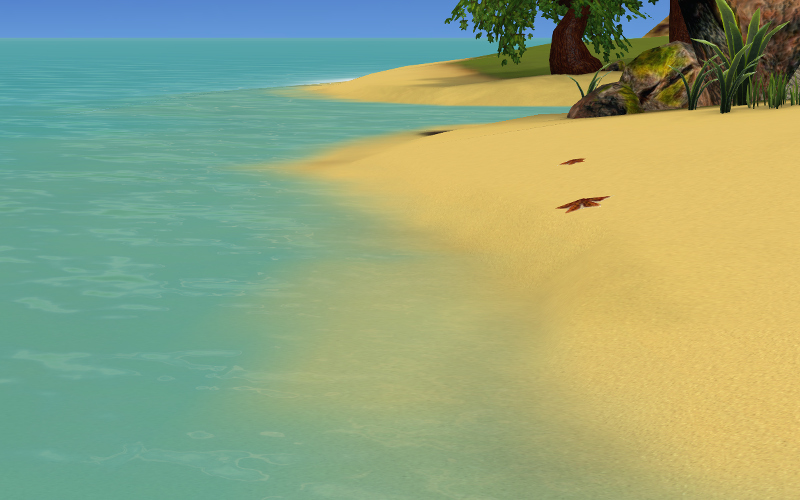
\includegraphics[width=1.000\linewidth]{alpha_map_water.jpg}\hfill}

\begin{DUlineblock}{0em}
\item[] 
\end{DUlineblock}

\index{textures!stencil map}\index{stencil map}

\section{Stencil map}
\label{textures:stencil-map}\label{textures:index-9}
The special purpose texture (colorful or grayscale) contains information about other textures surface distribution.


\subsection{Activation}
\label{textures:id14}\begin{enumerate}
\item {} 
In case of node materials a stencil map should be used in the corresponding node structure.

\item {} 
In case of generic materials a stencil map should be located in a texture slot between two mixing diffuse textures. A stencil map requires to set both the \code{RGB to Intensity} and the \code{Stencil} checkboxes on the \code{Textures \textgreater{} Influence} panel.

\end{enumerate}


\subsection{Additional settings}
\label{textures:id15}
In the case of generic materials one of the mixing diffuse textures can have the \code{Normal} (``matcap'') texture coordinates type.


\subsection{Limitations}
\label{textures:id16}
In case of generic materials the engine only interprets the red channel of a stencil map. A specular map or a normal map (if any) are not mixing. The \code{Mapping \textgreater{} Size} setting is extracted from the first texture and is applied to the all remaining textures.


\subsection{The example}
\label{textures:id17}
The apple model material has the following textures: the normal map, the diffuse texture with the specular map in its alpha channel, the stencil map, the diffuse ``matcap'' map, the environment map.

{\hfill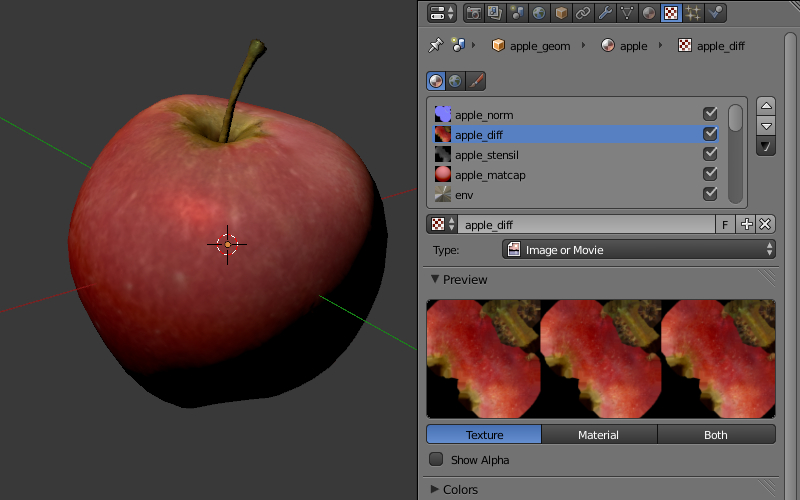
\includegraphics[width=1.000\linewidth]{stencil_apple.jpg}\hfill}

\begin{DUlineblock}{0em}
\item[] 
\end{DUlineblock}

{\hfill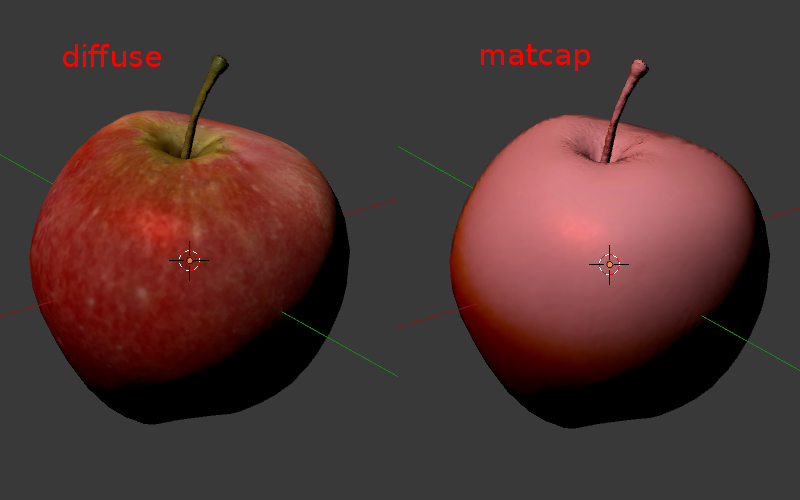
\includegraphics[width=1.000\linewidth]{stencil_apple_separate_textures.jpg}\hfill}

\begin{DUlineblock}{0em}
\item[] 
\end{DUlineblock}

\index{textures!environment map}\index{environment map}

\section{Environment map}
\label{textures:environment-map}\label{textures:index-10}
An environment map is used as a mirror map and as a static sky texture (skydome).

The engine considers it as a cube texture. Environment map bitmaps should contain 6 projected environment images, packed in 2 rows by 3 (a Blender format). Bitmap dimensions for each image should respect the 2$^{\text{N}}$ rule (512, 1024 etc).

It is recommended to use the lossless format (PNG) in order to avoid seams.

{\hfill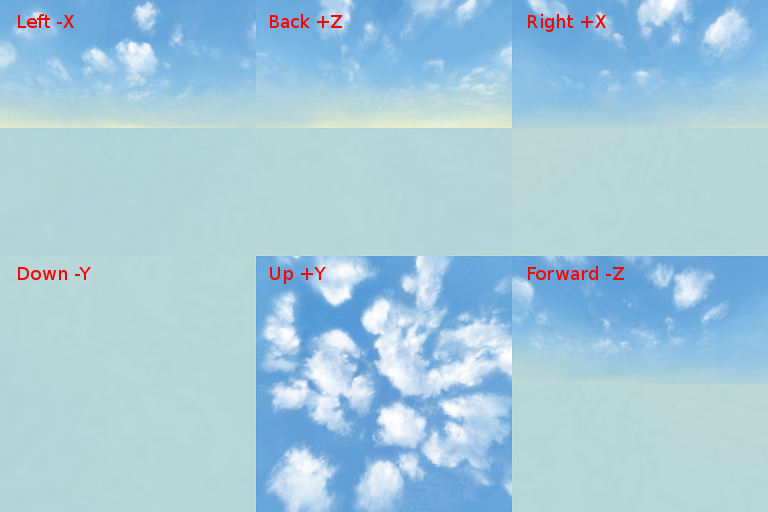
\includegraphics[width=1.000\linewidth]{environment_map.png}\hfill}


\subsection{Environment map creation}
\label{textures:id18}
Blender has option for baking a scene into an environment map. To do this:
\begin{enumerate}
\item {} 
Create a scene for baking.

\item {} 
Add an empty object to the desirable viewing center (\code{Add \textgreater{} Empty}).

\item {} 
Go to the \code{World} tab then to the \code{Textures} tab and create a new texture with the \code{Environment Map} type.

\item {} 
On the \code{Environment Map} panel select the \code{Static} source, then select the empty object in the \code{Viewport Object} field, the set the 2$^{\text{N}}$ dimension (512, 1024 etc).

\item {} 
Render the scene with \code{F12} (a camera should exist).

\item {} 
Save the environment map into a file.

\end{enumerate}

{\hfill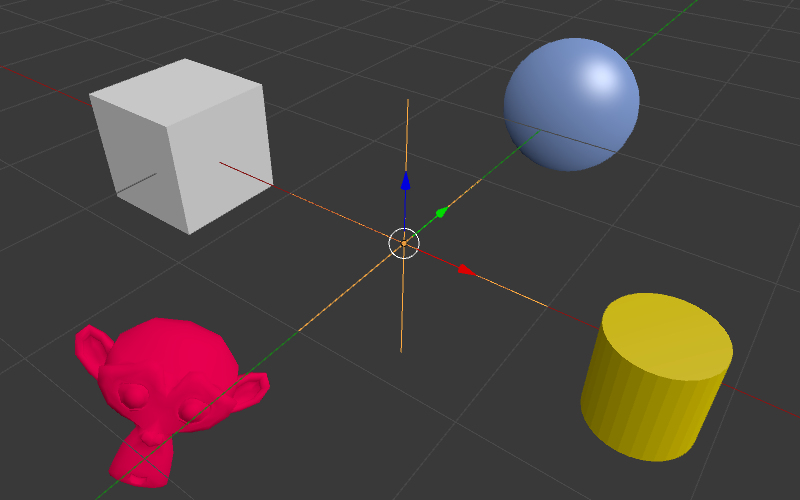
\includegraphics[width=1.000\linewidth]{environment_map_baking_scene.jpg}\hfill}

\begin{DUlineblock}{0em}
\item[] 
\end{DUlineblock}

{\hfill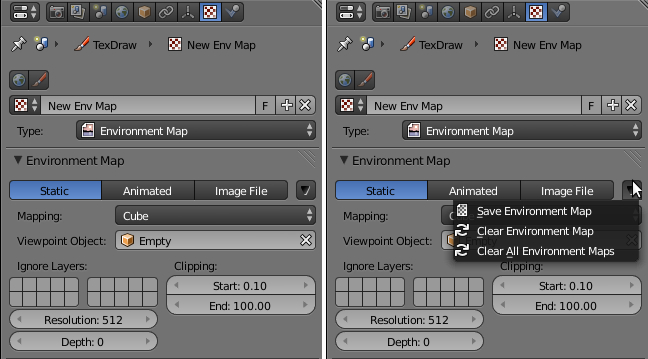
\includegraphics[width=1.000\linewidth]{environment_map_baking_ui.jpg}\hfill}

\index{textures!mirror map}\index{mirror map}

\section{Mirror map}
\label{textures:id19}\label{textures:mirror-map}\label{textures:index-11}
A mirror map is used for visualization of surface reflection. It is an environment map.


\subsection{Activation}
\label{textures:id20}
Select the \code{Environment Map} texture type (\code{Type}) . Set the \code{Shading \textgreater{} Mirror} checkbox on the \code{Textures \textgreater{} Influence} panel.


\subsection{Additional settings}
\label{textures:id21}\begin{description}
\item[{\emph{Influence \textgreater{} Shading \textgreater{} Mirror}}] \leavevmode
Influence of the mirror map on reflection. The default value is 1.0.

\end{description}


\strong{See also:}


{\hyperref[materials:reflection-static]{\emph{Static reflection}}}.



\index{textures!sky}\index{skydome}

\section{Skydome}
\label{textures:skydome}\label{textures:skydome-texture}\label{textures:index-12}
A skydome is used for sky visualization. It is an environment map.


\subsection{Activation}
\label{textures:id22}
Create a specifically oriented plane model. Create material and set the \code{Blend4Web \textgreater{} Special: Skydome} checkbox. Create the \code{Environment Map} texture.


\subsection{Additional settings}
\label{textures:id23}
Set the \code{Blend4Web \textgreater{} Disable frustum culling} checkbox for the plane object in order to avoid image disappearance upon camera rotation.

{\hfill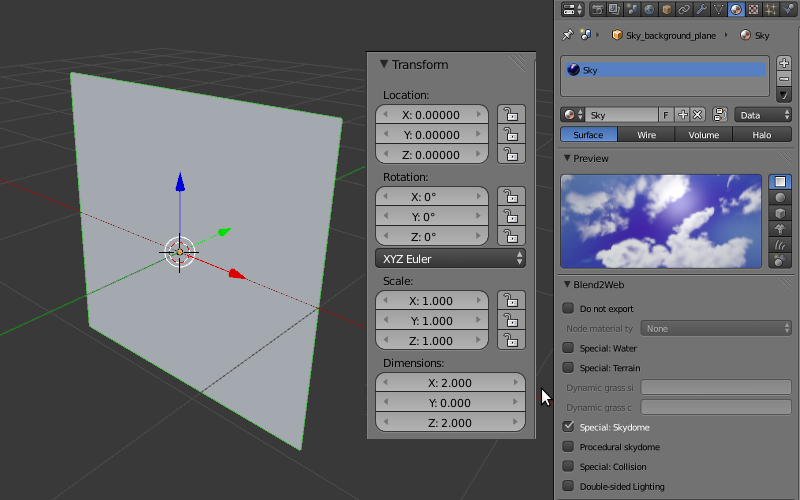
\includegraphics[width=1.000\linewidth]{skydome.jpg}\hfill}

\begin{DUlineblock}{0em}
\item[] 
\end{DUlineblock}
\phantomsection\label{textures:render-to-texture}
\index{textures!render to}\index{render-to-texture}\index{RTT}

\section{Render-to-texture, RTT}
\label{textures:render-to-texture-rtt}\label{textures:index-13}
A 3D scene real-time rendered image can be used as a texture by an object from another scene (``main'' scene).


\subsection{Activation}
\label{textures:id24}\begin{enumerate}
\item {} 
Create an additional source scene, rename it for convenience, create a \code{World}, add the objects wanted, setup camera view.

\item {} 
Set the \code{None} type for a texture of the target object on the main scene, and specify the source scene name in the \code{Blend4Web \textgreater{} Source scene} field. Select the \code{UV} in the \code{Mapping \textgreater{} Coordinates} menu. Make sure that the target object mesh has a UV map.

\end{enumerate}

{\hfill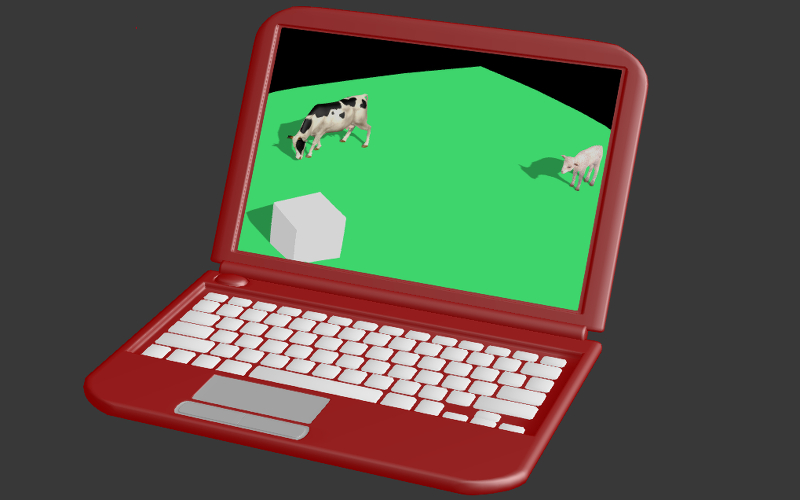
\includegraphics[width=1.000\linewidth]{render_to_texture.jpg}\hfill}


\subsection{Limitations}
\label{textures:id25}
Note that there is a bug at the moment which requires both scenes to have at least one shared light source.
\phantomsection\label{materials:materials}
\index{materials}

\chapter{Materials}
\label{materials:index-0}\label{materials::doc}\label{materials:id1}
Materials describe object surface response to light and also contain information about surface transparency, reflectivity, physical parameters and other.

Meshes can have one or more materials. In case of multiple materials they can be assigned to different polygons in \code{Edit Mode}. To do this select the needed polygons, select the needed material from the list and click the \code{Assign} button.

The following materials types are supported: \code{Surface}, \code{Halo}.

\index{materials!shading parameters}

\section{Lighting parameters}
\label{materials:id2}\label{materials:index-1}\label{materials:material-lighting-params}\begin{figure}[htbp]
\centering

\scalebox{0.500000}{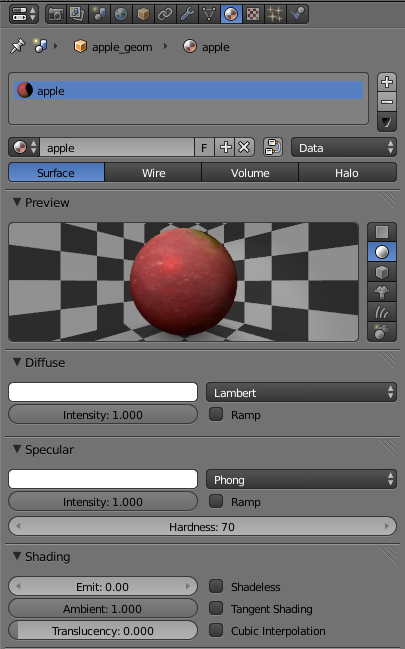
\includegraphics{material_panel_shading.jpg}}
\end{figure}
\begin{description}
\item[{\emph{Diffuse \textgreater{} Color}}] \leavevmode
Diffuse light color. The default value is (0.8, 0.8, 0.8). It may interact with the diffuse map color.

\item[{\emph{Diffuse \textgreater{} Intensity}}] \leavevmode
Diffuse light intensity. The default value is 0.8.

\item[{\emph{Diffuse \textgreater{} Shader}}] \leavevmode
Diffuse shading algorithm. The engine supports the following algorithms: \code{Lambert}, \code{Oren-Nayar}, \code{Fresnel}. The default value is \code{Lambert}.

\item[{\emph{Specular \textgreater{} Color}}] \leavevmode
Specular light color. The default value is (1.0, 1.0, 1.0). It may interact with the specular map color.

\item[{\emph{Specular \textgreater{} Intensity}}] \leavevmode
Specular light intensity. The default value is 0.5.

\item[{\emph{Specular \textgreater{} Hardness}}] \leavevmode
Exponent in specular shading calculation formula. The default value is 50. Note that the formula used in the engine differs slightly from the Blender one.

\item[{\emph{Specular \textgreater{} Shader}}] \leavevmode
Specular shading algorithm. The engine supports the following algorithms: \code{CookTorr}, \code{Phong} - both are treated as the same, and \code{WardIso}. The default value is \code{CookTorr}.

\item[{\emph{Shading \textgreater{} Emit}}] \leavevmode
Emission intensity. The default value is 0.0.

\item[{\emph{Shading \textgreater{} Ambient}}] \leavevmode
Ambient influence factor on material. The default value is 1.0.

\item[{\emph{Shading \textgreater{} Shadeless}}] \leavevmode
When turned on a material doesn't react to light. Turned off by default.

\item[{\emph{Game Settings \textgreater{} Backface Culling}}] \leavevmode
When turned on poligons' back faces are not rendered by the engine. Turned on by default.

\item[{\emph{Options \textgreater{} Vertex Color Paint}}] \leavevmode
Mesh vertex color is used instead of material diffuse color when the checkbox is turned on.

\end{description}

\index{materials!transparency}\index{transparency}

\section{Transparency}
\label{materials:id3}\label{materials:index-2}
\index{transparency!types}

\subsection{Types}
\label{materials:id4}\label{materials:index-3}
Transparency implementation type can be selected in the \code{Alpha Blend} menu on the \code{Materials \textgreater{} Game Settings} panel (in the \code{Blender Game} mode).

The engine supports the following transparency implementation types (sorted in the ascending order by performance):
\begin{description}
\item[{\emph{Alpha Sort}}] \leavevmode
Transparent with gradient. The engine performs sorting of triangles by camera distance in order to render overlapping transparent surfaces correctly. This operation is computationally expensive. It is recommended to use this feature for closed transparent geometry (bottle, car glass etc).

\item[{\emph{Alpha Blend}}] \leavevmode
Transparent with gradient. Triangles sorting is not performed. It is recommended to use this feature for unclosed transparent geometry (water surface, decals).

\item[{\emph{Add}}] \leavevmode
Transparent with gradient. Triangles sorting is not performed. The engine turns off writing to the depth buffer which causes rendering of transparent surfaces in arbitrary order. It is recommended to use this feature for effects (particle systems, glowing beams).

\item[{\emph{Alpha Clip}}] \leavevmode
Transparent without gradient. The engine discards pixels when their alpha is less than 0.5. Triangles sorting is not performed. It is recommended to use this feature with a mask texture for visualization of smaller details (tree leaves, grass).

\item[{\emph{Opaque}}] \leavevmode
Non-transparent. Alpha is ignored. This is the default value.

\end{description}

{\hfill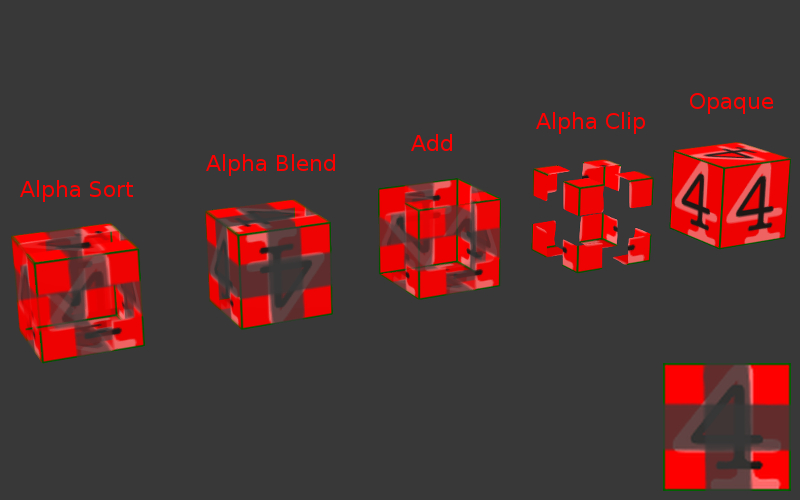
\includegraphics[width=1.000\linewidth]{alpha_types.jpg}\hfill}

\index{transparency!setup}

\subsection{Additional settings}
\label{materials:index-4}\label{materials:id5}\begin{description}
\item[{\emph{Transparency}}] \leavevmode
Setting the transparency checkbox is required for viewing transparent objects in Blender. The engine ignores this option - the \code{Alpha Blend} option is used instead.

\item[{\emph{Transparency \textgreater{} Alpha}}] \leavevmode
Material transparency level. The engine ignores this parameter (in contrast to Blender) if there is a diffuse texture - alpha channel values of a texture are used instead.

\item[{\emph{Options \textgreater{} Z Offset}, depth offset}] \leavevmode
This option explicitly specifies relative positioning order of objects with \textbf{different} materials with the purpose of depth sorting. The option can take both negative and positive values. The more distant is object the lesser parameter value should be to provide correct rendering. The default value is 0.0.

\item[{\emph{Transparency \textgreater{} Fresnel}}] \leavevmode
Fresnel power for transparency. It is exported but is not used at the moment.

\item[{\emph{Transparency \textgreater{} Blend}}] \leavevmode
Fresnel factor for transparency. It is exported but is not used at the moment.

\end{description}

\index{materials!reflection}\index{reflection}

\section{Reflection}
\label{materials:id6}\label{materials:index-5}\label{materials:material-mirror}
\index{reflection!static}

\subsection{Static reflection}
\label{materials:id7}\label{materials:index-6}\label{materials:reflection-static}
A surface reflects the same image no matter how environment changes. For activation simply use the {\hyperref[textures:mirror-map]{\emph{mirror map}}}.


\strong{See also:}


{\hyperref[materials:fresnel]{\emph{Fresnel effect for reflection}}}



\index{reflection!dynamic}

\subsection{Dynamic reflection}
\label{materials:index-7}\label{materials:id8}
A surface reflects the selected objects in their current position. Only reflection in a plane is supported.


\subsubsection{Activation}
\label{materials:id9}\begin{enumerate}
\item {} 
Set the \code{Render reflections} checkbox on the \code{Scene \textgreater{} Blend4Web} panel.

\item {} 
Add an empty object as a reflection plane by executing for example{}`{}`Add \textgreater{} Empty \textgreater{} Single Arrow{}`{}`. Rename it for convenience.

\item {} 
For \emph{reflective} objects set the \code{Reflective} checkbox on the \code{Object \textgreater{} Blend4Web} panel and specify the empty object name in the \code{Reflection plane} field.

\item {} 
For the needed materials of the \emph{reflective} objects set the \code{Mirror \textgreater{} Reflectivity} value.

\item {} 
For the \emph{reflexible} objects set the checkbox \code{Reflexible} on the \code{Object \textgreater{} Blend4Web} panel.

\end{enumerate}

\begin{notice}{note}{Note:}
It is also recommended to turn on the \code{World \textgreater{} Environment Lighting} checkbox.
\end{notice}


\subsubsection{Limitations}
\label{materials:id10}
Normal maps and shadows are ignored in the reflected image for optimization purposes.


\strong{See also:}


{\hyperref[materials:fresnel]{\emph{Fresnel effect for reflection}}}



\index{reflection!Fresnel effect}\index{Fresnel effect}

\subsection{Fresnel effect for reflection}
\label{materials:id11}\label{materials:fresnel}\label{materials:index-8}
The Fresnel effect is dependency on angle of incidence for transmitted and reflected light intencity. If angle of incidence is close to zero (i.e. light falls almost at right angle to surface) the transmitted light portion is large and the reflected light portion is small. On the contrary if angle of incidence is close to 90 degrees (i.e. light falls almost parallel to surface) almost all light is reflected.

The engine uses approximate Schlick's formula:
\begin{quote}

R = R$_{\text{0}}$ + (1 − R$_{\text{0}}$)(1 - cos \(\theta\))$^{\text{N}}$, where

R - reflection coefficient,

R$_{\text{0}}$ - reflection coefficient in case of viewing at right angle to surface (i.e. when \(\theta\) = 0),

\(\theta\) - angle of incidence (equal to angle of reflection, which is angle of between light direction and camera direction), it is calculated by the engine in real-time,

N - exponent.
\end{quote}


\subsubsection{Setting}
\label{materials:id12}
Fresnel effect can be setup both for static and dynamic reflection.
\begin{description}
\item[{\emph{Mirror \textgreater{} Fresnel}}] \leavevmode
Fresnel power for reflection. This is exponent N in Schlick's formula. In Blender it is limited by values from 0 to 5. If this parameter equals to zero Fresnel effect is not observed, the \emph{full} reflection at all angles occurs. If this parameter is more than zero, a material is less reflective when viewing surface at angles which are close to right angle. The bigger this parameter the bigger the angle deviation from the right angle for which Fresnel effect is observed.

\item[{\emph{Mirror \textgreater{} Blend}}] \leavevmode
Fresnel factor for reflection. It transfers to R$_{\text{0}}$ in Schlick's formula by the following expression: R$_{\text{0}}$ = 1 - \code{Blend} / 5. In Blender it is limited by values from 0 to 5. This parameter defines Fresnel effect intensity: the bigger the \code{Blend} factor, the more the Fresnel effect influence. If it is equal to zero Fresnel effect is not observed.

\end{description}

{\hfill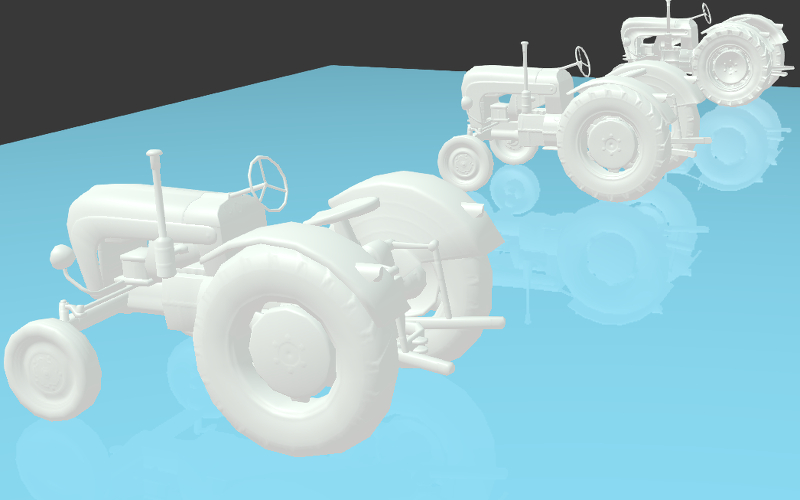
\includegraphics[width=1.000\linewidth]{reflection_dynamic_and_fresnel.jpg}\hfill}

\begin{DUlineblock}{0em}
\item[] 
\end{DUlineblock}

\index{materials!special parameters}

\section{Parameters specific to the engine}
\label{materials:id13}\label{materials:index-9}
Located on the \code{Blend4Web} panel.
\begin{description}
\item[{\emph{Do not export}}] \leavevmode
Material is not to be exported.

\item[{\emph{Special: Water}}] \leavevmode
Special material for water rendering.

\item[{\emph{Special: Skydome}}] \leavevmode
Special material for sky rendering.


\strong{See also:}


{\hyperref[textures:skydome-texture]{\emph{Skydome}}}



\item[{\emph{Special: Collision}}] \leavevmode
Special material for collision geometry.


\strong{See also:}


{\hyperref[physics:physics]{\emph{Физика}}}



\item[{\emph{Double-sided Lighting}}] \leavevmode
Turns on the double-sided lighting mode. The option is useful for non-transparent objects with single layered mesh.

\end{description}

\index{materials!halo}\index{halo}

\section{Halo materials}
\label{materials:material-halo}\label{materials:index-10}\label{materials:halo}
Halo materials are used in particle systems and in static meshes. Below the halo use in static meshes is considered.


\subsection{Activation}
\label{materials:id14}
Select \code{Halo} type in the \code{Materials} tab. It's also recommended to select the transparency type with gradient (\code{Add}, \code{Alpha Blend} or \code{Alpha Sort}).

{\hfill
\includegraphics[width=1.000\linewidth]{halo.jpg}\hfill}


\subsection{Additional settings}
\label{materials:id15}\begin{description}
\item[{\emph{Halo \textgreater{} Alpha}}] \leavevmode
Material transparency factor. The default value is 1.0 (non-transparent).

\item[{\emph{Halo \textgreater{} Color}}] \leavevmode
Material color. The default value is (0.8, 0.8, 0.8) (almost white).

\item[{\emph{Halo \textgreater{} Seed}}] \leavevmode
Unused.

\item[{\emph{Halo \textgreater{} Size}}] \leavevmode
Particle size. The default value is 0.5.

\item[{\emph{Halo \textgreater{} Hardness}}] \leavevmode
Exponent for computing gradient. Affects visible dimensions of particles. The default value is 50.

\item[{\emph{Halo \textgreater{} Add}}] \leavevmode
Unused.

\item[{\emph{Halo \textgreater{} Rings}}] \leavevmode
Use rings. Relative count and color can be setup.

\item[{\emph{Halo \textgreater{} Lines}}] \leavevmode
Use lines. Relative count and color can be setup.

\item[{\emph{Halo \textgreater{} Star Tips}}] \leavevmode
Use starts. Edges count can be setup.

\item[{\emph{Blend4Web \textgreater{} Special: Stars}}] \leavevmode
Turns on starry sky rendering mode while the mesh will be fixed relative to camera. Also it is required to set the \code{Blend4Web \textgreater{} Dynamic intensity} checkbox for a lamp. Applications must setup the hours of darkness via API.

\item[{\emph{Blend4Web \textgreater{} Blending Height}}] \leavevmode
Heights range for stars brightness fading.

\item[{\emph{Blend4Web \textgreater{} Stars Minimum Height}}] \leavevmode
Minimum height in the object's local space at which stars are visible.

\end{description}
\phantomsection\label{node_materials:node-materials}
\index{node materials}

\chapter{Node materials}
\label{node_materials:index-0}\label{node_materials::doc}\label{node_materials:id1}
Shader nodes extend significantly potential of Blender's standard materials by means of considering shading as a batch of basic transformations.

\index{materials!nodes}

\section{Standard nodes}
\label{node_materials:id2}\label{node_materials:index-1}\label{node_materials:generic-node-materials}
\index{materials!nodes}
All Blender functions are supported excepting the following cases:
\begin{itemize}
\item {} 
\code{Geometry} - the \code{Local}, \code{Orco} and \code{Vertex Alpha} outputs are not supported.

\item {} 
\code{Material}, \code{Extended Material} - allowed no more than one node per material; the \code{Refl}, \code{Ambient}, \code{SpecTra}, \code{Ray Mirror} inputs are not supported; the \code{AO} output is not supported.

\item {} 
\code{RGB Curves} is not supported.

\item {} 
\code{Vector Curves} is not supported.

\end{itemize}

In addition a poor performance of some nodes in real-time context should be taken into account. It is not recommended to use the following nodes:
\begin{itemize}
\item {} 
\code{Hue/Saturation}

\item {} 
\code{MixRGB} - the \code{Burn}, \code{Dodge}, \code{Value}, \code{Saturation}, \code{Hue}, \code{Color} types.

\end{itemize}

It is not recommended to create too complex materials especially if they use many \code{Geometry} or \code{Texture} nodes.


\section{Special nodes}
\label{node_materials:custom-node-materials}\label{node_materials:id3}
\index{materials!nodes}
Special nodes extend standard nodes functionality in order to support the engine features. Special nodes are created as node groups (\code{Node groups} or \code{Node tree}) with the determined names and input formats. All special nodes are collected in the \code{special\_nodes.blend} file for convenience.


\subsection{LINEAR\_TO\_SRGB and LINEAR\_TO\_SRGB}
\label{node_materials:linear-to-srgb-linear-to-srgb}
Color correction from linear color space to sRGB space and back.


\strong{See also:}


{\hyperref[gamma_alpha:gamma-nodes]{\emph{Коррекция в нодовых материалах}}}




\subsection{REPLACE}
\label{node_materials:replace}
The node performs replacing of inputs depending on working environment (i.e. Blender vieport or Blend4Web). When working in Blender the \code{Color1} input is connected to the \code{Color} output and the \code{Color2} input is ignored. On the contrary when working in the engine the inputs are interchanged (the \code{Color1} one is ignored and the \code{Color2} one is connected to the output). The node is intended for displaying one node structure in the viewport and another - in the engine.

It is used normally for normal mapping. Blender node materials do not support a tangent space. Therefore the only possible method to display normal maps in the viewport correctly is their usage inside Material nodes.


\subsection{CLAMP}
\label{node_materials:clamp}
The node limits the output value. As a result all the output vector components take values from 0 to 1 inclusive.


\subsection{NORMAL\_VIEW}
\label{node_materials:normal-view}
The node transforms a normal into the camera coordinate space. Transformation is necessary because the engine defines all normals in the world coordinate space. A normal should be used only for effects and not for connection to output of the \code{Material} or \code{Extended Material} nodes.


\subsection{PARALLAX}
\label{node_materials:parallax}
The node implements texture coordinates offset using a height map.


\subsubsection{Input parameters}
\label{node_materials:id4}\begin{description}
\item[{\emph{UV}}] \leavevmode
Source texture coordinates

\item[{\emph{Height}}] \leavevmode
RGBA texture with a height map packed into the alpha channel

\item[{\emph{Scale}}] \leavevmode
Texture coordinates offset factor

\item[{\emph{Steps}}] \leavevmode
The number of steps for iterative generation of texture coordinates offset. The bigger this value the better final quality.

\end{description}


\subsubsection{Output parameters}
\label{node_materials:id5}\begin{description}
\item[{\emph{UV}}] \leavevmode
Resulting texture coordinates which are used as input for texture nodes.

\end{description}


\subsection{TRANSLUCENCY}
\label{node_materials:translucency}
The node implements translucency effect (with respect to light sources only) for thin objects such as cloth, leaves, paper etc. The effects consists of two parts: 1) brightening of the object side which is opposite to the light source and 2) appearance of a light spot right in the light source place.


\subsubsection{Input parameters}
\label{node_materials:id6}\begin{description}
\item[{\emph{Color}}] \leavevmode
One-channel texture which defines material heterogeneity - white color denotes maximum translucency effect while black color denotes its absence. White color is used by default.

\item[{\emph{Backside Factor}}] \leavevmode
Material color correction coefficient for the side which is opposite to the light source. It describes color richness effect for translucent areas.
\begin{itemize}
\item {} 
\emph{Backside Factor \textless{} 1} - brightening

\item {} 
\emph{Backside Factor = 1} - no correction

\item {} 
\emph{Backside Factor \textgreater{} 1} - darkening

\end{itemize}

The default value is 1.

\item[{\emph{Spot Hardness}}] \leavevmode
Light spot blurring factor. The bigger this value the smaller spot and the sharper spot edges. The default value is 1000.

\item[{\emph{Spot Intensity}}] \leavevmode
Light spot intesity. The bigger this value the brighter light spot. The default value is 1.

\item[{\emph{Spot Diffuse Factor}}] \leavevmode
Material diffuse color influence on light spot color.
\begin{itemize}
\item {} 
\emph{Spot Diffuse Factor = 0} - light spot color is diffuse color

\item {} 
\emph{Spot Diffuse Factor = 1} - light spot color is white

\end{itemize}

The default value is 1.

\end{description}


\subsubsection{Output parameters}
\label{node_materials:id7}\begin{description}
\item[{\emph{Translucency}}] \leavevmode
The output should be connected to the \code{Translucency} input of a \code{Extended Material} node.

\end{description}
\phantomsection\label{lighting:lighting}
\index{lighting}

\chapter{Lighting and shadows}
\label{lighting:index-0}\label{lighting::doc}\label{lighting:id1}
\index{light sources}

\section{Illumination by light sources}
\label{lighting:id2}\label{lighting:index-1}
A scene can have multiple (but not less than one) light sources of different types.


\subsection{Light source types}
\label{lighting:id3}
The following light source types are supported:
\begin{description}
\item[{\emph{Point}}] \leavevmode
Light propagates from one point uniformly to all directions with gradual attenuation.

\item[{\emph{Sun}}] \leavevmode
Light propagates from an infinite plane in one direction without attenuation.

\item[{\emph{Spot}}] \leavevmode
Light propagates from one point within angular limit, with gradual attenuation.

\item[{\emph{Hemi}}] \leavevmode
Hemispherical. Light propagates from an infinite hemisphere without attenuation.

\end{description}


\subsection{Light source setup}
\label{lighting:id4}
Performed in the \code{Object Data} tab when a lamp object is selected.

{\hfill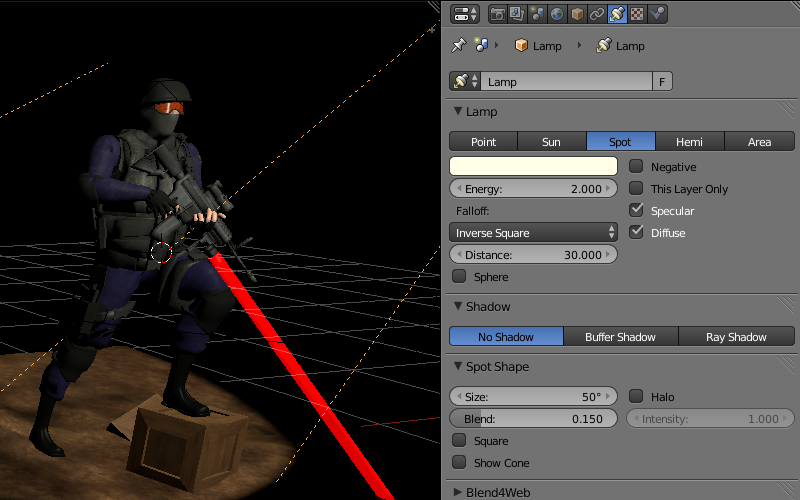
\includegraphics[width=1.000\linewidth]{lighting_setup.jpg}\hfill}

\begin{DUlineblock}{0em}
\item[] 
\end{DUlineblock}
\begin{description}
\item[{\emph{Color}}] \leavevmode
Light color. The default value is (1.0, 1.0, 1.0) (i.e. white).

\item[{\emph{Energy}}] \leavevmode
Radiation intensity. The default value is 1.0.

\item[{\emph{Falloff}}] \leavevmode
Attenuation type. The value is exported but the engine always uses \code{Inverse Square}. It is applicable for the \code{Point} and \code{Spot} light source types. The default value is \code{Inverse Square}.

\item[{\emph{Distance}}] \leavevmode
Attenuation parameter. It is applicable for the \code{Point} and \code{Spot} light source types. The default value is 25.0.

\item[{\emph{Spot Shape \textgreater{} Size}}] \leavevmode
Cone angle in degrees. It is applicable for the \code{Spot} light source type. The default value is 45º.

\item[{\emph{Spot Shape \textgreater{} Blend}}] \leavevmode
Parameter for blurring of light spot edges. It is applicable for the \code{Spot} light source type. The default value is 0.15.

\item[{\emph{Blend4Web \textgreater{} Do not export}}] \leavevmode
Don't export the light source. Turned off by default.

\item[{\emph{Blend4Web \textgreater{} Generate shadows}}] \leavevmode
Use this light source for shadow calculation. Should be used when multiple light sources present. Turned off by default.

\item[{\emph{Blend4Web \textgreater{} Dynamic intesity}}] \leavevmode
Use this light source for daytime calculation. Applicable only for the \code{Sun} light source type. Turned off by default.

\end{description}


\section{Ambient lighting}
\label{lighting:id5}
The engine uses a simple hemispherical lighting model in which horizon and zenith colors should be specified.


\subsection{Activation}
\label{lighting:id6}
Set the \code{Environment Lighting} checkbox on the \code{World} tab.

{\hfill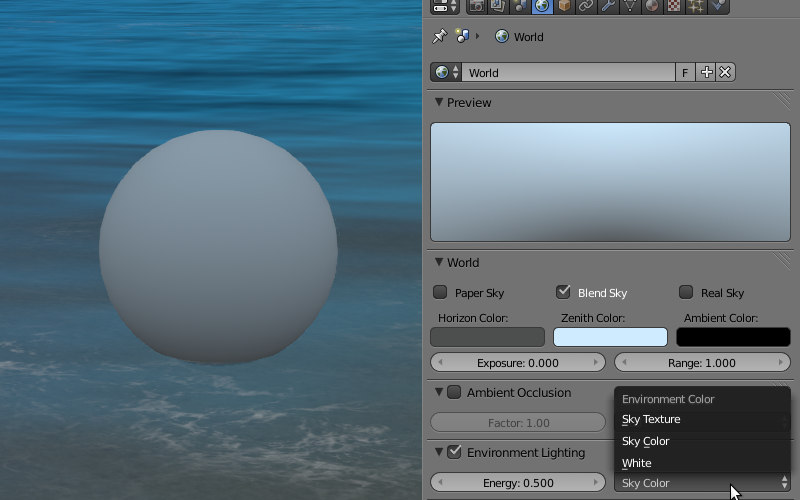
\includegraphics[width=1.000\linewidth]{lighting_environment.jpg}\hfill}


\subsection{Setup}
\label{lighting:id7}\begin{description}
\item[{\emph{Environment Lighting \textgreater{} Energy}}] \leavevmode
Ambient lighting intensity. The default value is 1.0.

\item[{\emph{Environment Lighting \textgreater{} Environment Color}}] \leavevmode
Ambient lighting source type - the supported types are \code{White} and \code{Sky Color}. If the \code{White} type is selected both horizon and zenith colors are white. If the \code{Sky Color} type is selected horizon and zenith colors can be specified by means of the \code{World \textgreater{} Horizon Color} and \code{World \textgreater{} Zenith Color} color pickers. The default value is \code{White}.

\item[{\emph{World \textgreater{} Horizon Color} and \emph{World \textgreater{} Zenith Color}}] \leavevmode
Horizon and zenith colors. It is recommnended to activate the \code{World \textgreater{} Blend Sky} option for better color selection.

\end{description}


\section{Shadows}
\label{lighting:id8}

\subsection{Activation}
\label{lighting:id9}\begin{enumerate}
\item {} 
Set the \code{Blend4Web \textgreater{} Shadows Cast} checkbox in the \code{Object} tab for objects which \textbf{cast} shadows.

\item {} 
Set the \code{Blend4Web \textgreater{} Shadows Receive} checkbox in the \code{Object} tab for objects which \textbf{receive} shadows.

\item {} 
Make sure that the \code{Blend4Web \textgreater{} Render shadows} checkbox in the \code{Scene} tab is set.

\end{enumerate}


\subsection{Setup}
\label{lighting:id10}\begin{description}
\item[{\emph{Direction}}] \leavevmode
If there are multiple light sources it is recommended to specify the exact light source which is used for shadow calculations, by enabling the \code{Blend4Web \textgreater{} Generate shadows} option in the \code{Object Data} tab for the selected lamp object.

\item[{\emph{Color}}] \leavevmode
The shadow color is determined by ambient lighting settings.

\end{description}

There are the following additional settings on the \code{Blend4Web \textgreater{} Shadow Settings} panel of the \code{World} tab:
\begin{description}
\item[{\emph{Optimize shadow volume}}] \leavevmode
Optimize shadow volume which is used for shadow calculation. If the checkbox is set the engine performs shadow volume optimization taking into account bounding volume of casting objects. This improves shadow quality on smaller scenes. If the option is disabled such optimization doesn't occur. This improves shadow quality on extensive scenes. This option is enabled by default.

\end{description}


\subsubsection{Cascades}
\label{lighting:id11}
In order to provide acceptable shadow quality and to cover considerable space at the same time it is required to use multiple stages for shadow generation (cascades). Thus a cascade with best quality is situated near the observer and a cascade with worst quality is in the distance.

{\hfill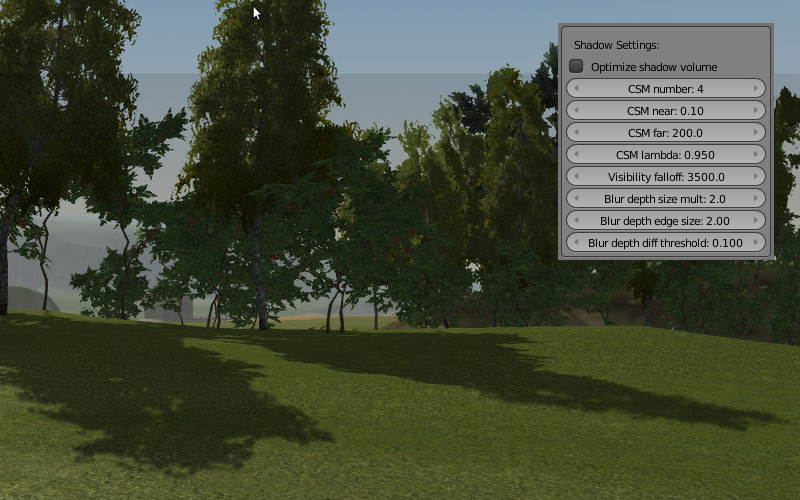
\includegraphics[width=1.000\linewidth]{shadow_cascades.jpg}\hfill}

\begin{DUlineblock}{0em}
\item[] 
\end{DUlineblock}
\begin{description}
\item[{\emph{CSM number}}] \leavevmode
Number of shadow cascades. Supported from 1 to 4 cascades. The default value is 3.

\item[{\emph{CSM near}}] \leavevmode
Shadow rendering near boundary. The default value is 0.1.

\item[{\emph{CSM far}}] \leavevmode
Shadow rendering far boundary. The default value is 100.

\item[{\emph{CSM lambda}}] \leavevmode
Cascade boundaries distribution factor. The values for calculated cascade boundaries are displayed in viewer in the \code{Shadows} tab. The default value is 0.875.

\end{description}


\subsubsection{Softened shadows}
\label{lighting:id12}\begin{description}
\item[{\emph{Visibility falloff}}] \leavevmode
Factor for exponential decay of shadow visibility which is depending on distance between casting and receiving points. It is used for reduction of self-shadowing artefacts (i.e. when castor and receiver are the same object). The default value is 3500.0.

\item[{\emph{Blur depth size mult}}] \leavevmode
Blur kernel size. Affects the shadow softening ratio. The default value is 1.0.

\item[{\emph{Blur depth edge size}}] \leavevmode
Difference between samples (in texels) for edge detection algorithm. Decreases haloing by excluding edges from blurring. The default value is 2.0.

\item[{\emph{Blur depth diff threshold}}] \leavevmode
Maximum of depth difference for edge detection algorithm multiplied by 1000. Decreases haloing by excluding edges from blurring. The default value is 0.1.

\end{description}


\chapter{Postprocessing effects}
\label{postprocessing_effects:postprocessing-effects}\label{postprocessing_effects::doc}\label{postprocessing_effects:id1}
\index{motion blur}\index{motion blur}

\section{Motion blur}
\label{postprocessing_effects:id2}\label{postprocessing_effects:motion-blur}\label{postprocessing_effects:index-0}
The motion blur effect can be used to improve realism of an interactive scene. It is showed as picture blurring when camera or objects move.


\subsection{Activation}
\label{postprocessing_effects:id3}
Set the \code{Enable Motion Blur} checkbox on the \code{Scene \textgreater{} Blend4Web} panel.


\subsection{Additional settings}
\label{postprocessing_effects:id4}
On the \code{World \textgreater{} Blend4Web \textgreater{} Motion blur settings} panel:
\begin{description}
\item[{\emph{Motion blur factor}}] \leavevmode
Effect appearance ratio. The higher this value the stronger motion blur.

\item[{\emph{Motion blur decay threshold}}] \leavevmode
Blur fade-out ratio. The higher this value the more distinct effect. The default value is 0.01.

\end{description}

{\hfill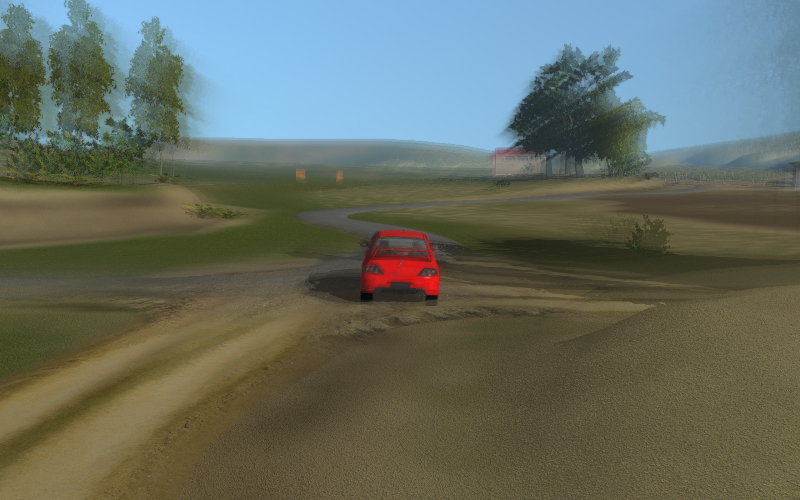
\includegraphics[width=1.000\linewidth]{motion_blur.jpg}\hfill}

\begin{DUlineblock}{0em}
\item[] 
\end{DUlineblock}

\index{depth of field}\index{depth of field}\index{DOF}

\section{Depth of field}
\label{postprocessing_effects:id5}\label{postprocessing_effects:dof}\label{postprocessing_effects:index-1}
The depth of field effect (DOF) can be used to accentuate a part of scene. It is showed as picture blurring nearer and farther the camera focus.


\subsection{Activation}
\label{postprocessing_effects:id6}\begin{enumerate}
\item {} 
Select an active camera and go to its settings panel (\code{Object Data}).

\item {} 
Then two options are available:
\begin{itemize}
\item {} 
Select an object for using as camera focus in the \code{Focus} menu of the \code{Depth of Field} panel. In this case moving away or approaching this object will cause the corresponding camera focus correction.

\item {} 
Set a non-zero value for the \code{Distance} on the \code{Depth of Field} panel (in Blender units = meters). In this case camera focus will be located at this distance from camera and will move together with it.

\end{itemize}

\end{enumerate}


\subsection{Additional settings}
\label{postprocessing_effects:id7}
On the \code{Object Data \textgreater{} Blend4Web} panel when active camera is selected:
\begin{description}
\item[{\emph{DOF front distance}}] \leavevmode
Distance from focus to the nearest plane (relative to camera) behind which full blurring occurs (in meters). The default value is 1.0.

\item[{\emph{DOF rear distance}}] \leavevmode
Distance from focus to the farthest plane (relative to camera) behind which full blurring occurs (in meters). The default value is 1.0.

\item[{\emph{DOF power}}] \leavevmode
Blurring ratio. The default value is 3.0.

\end{description}

{\hfill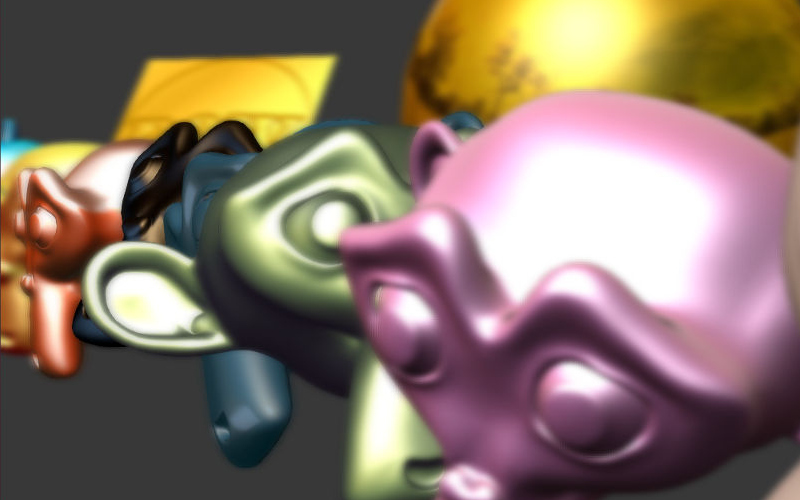
\includegraphics[width=1.000\linewidth]{dof.jpg}\hfill}

\begin{DUlineblock}{0em}
\item[] 
\end{DUlineblock}

\index{screen-space ambient occlusion}\index{screen-space ambient occlusion}\index{SSAO}

\section{Screen-space ambient occlusion}
\label{postprocessing_effects:index-2}\label{postprocessing_effects:ssao}\label{postprocessing_effects:id8}
Screen-space ambient occlusion (SSAO) effect can be used for faking complex light reflections from objects. The basis of this effect is that space between close objects is less accessible for diffuse light and hence is darker.


\subsection{Activation}
\label{postprocessing_effects:id9}
Set the \code{Enable SSAO} checkbox on the \code{Scene \textgreater{} Blend4Web} panel.


\subsection{Additional settings}
\label{postprocessing_effects:id10}
On the \code{World \textgreater{} Blend4Web \textgreater{} SSAO Settings} panel:
\begin{description}
\item[{\emph{Radius Increase}}] \leavevmode
Spherical sampling radius multiply factor when transfering from the internal sampling ring to the external one. The default value is 1.7.

\item[{\emph{Dithering Amount}}] \leavevmode
Ratio for random noise mixing used for strips reducing. The default value is 0.1.

\item[{\emph{Gauss Center}}] \leavevmode
Mathematical expectation - Gauss distribution parameter for depth difference between a pixel and a neighbouring sample. The default value is 0.2.

\item[{\emph{Gauss Width}}] \leavevmode
Standard deviation - Gauss distribution parameter for depth difference between a pixel and a neighbouring sample. The default value is 2.0.

\item[{\emph{Gauss Width Left}}] \leavevmode
Standard deviation in case depth difference is less than mathematical expectation. The default value is 0.1.

\item[{\emph{Influence}}] \leavevmode
SSAO appearance factor. The default value is 0.7.

\item[{\emph{Distance Factor}}] \leavevmode
Factor of SSAO appearance decay with distance. The default value is 0.0 (i.e. no decay).

\item[{\emph{Samples}}] \leavevmode
Number of samples (the more samples the better quality but the poorer performance). The default value is 16.

\end{description}

{\hfill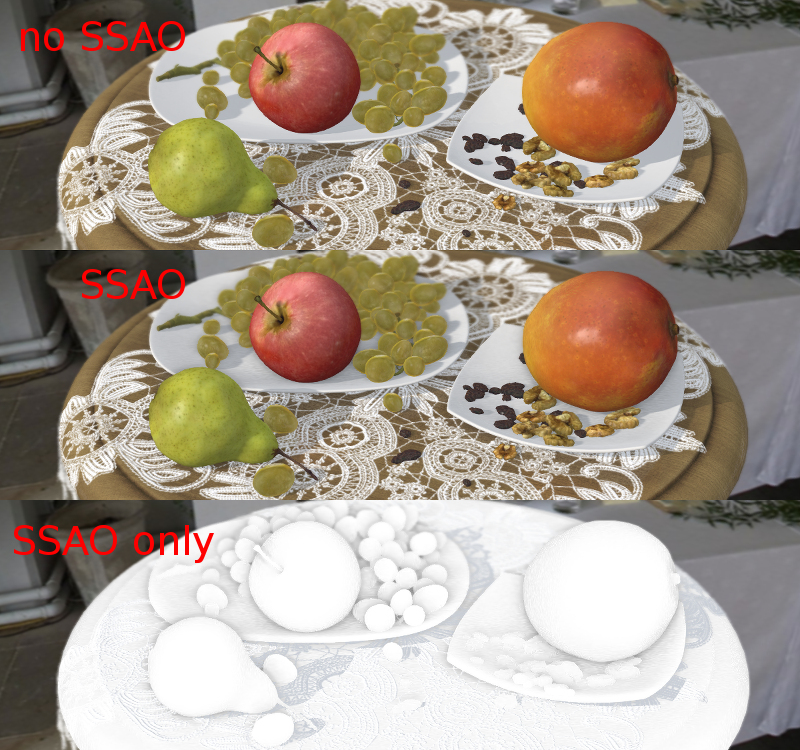
\includegraphics[width=1.000\linewidth]{ssao.jpg}\hfill}

\begin{DUlineblock}{0em}
\item[] 
\end{DUlineblock}

\index{crepuscular rays}\index{crepuscular rays}\index{god rays}

\section{God rays}
\label{postprocessing_effects:god-rays}\label{postprocessing_effects:id11}\label{postprocessing_effects:index-3}
God rays effect (aka crepuscular rays) simulates well-known natural appearance - visibility of illuminated air parts.


\subsection{Activation}
\label{postprocessing_effects:id12}
Set the \code{Enable God Rays} checkbox on the \code{Scene \textgreater{} Blend4Web} panel.


\subsection{Additional settings}
\label{postprocessing_effects:id13}
On the \code{World \textgreater{} Blend4Web \textgreater{} God Rays Settings} panel:
\begin{description}
\item[{\emph{God Rays Intensity}}] \leavevmode
The effect appearance factor. The default value is 0.7.

\item[{\emph{Maximum Ray Length}}] \leavevmode
Rays length factor. Defines a step between samples for radial blurring. The default value is 1.0.

\end{description}

{\hfill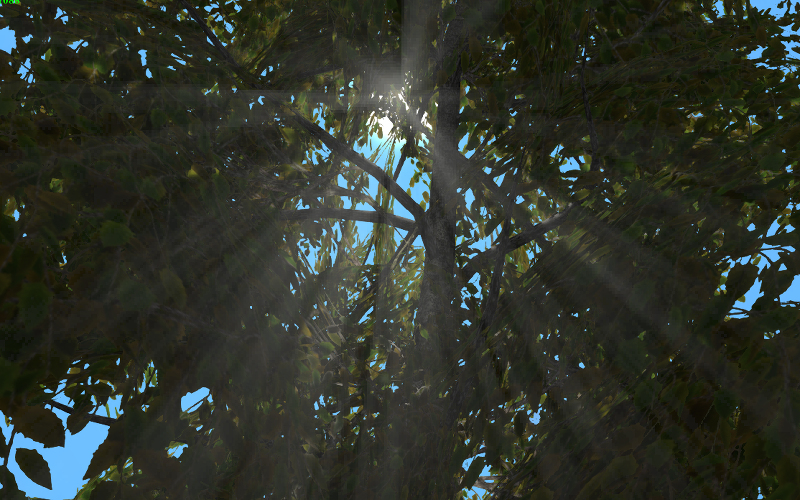
\includegraphics[width=1.000\linewidth]{god_rays.jpg}\hfill}

\begin{DUlineblock}{0em}
\item[] 
\end{DUlineblock}


\section{Bloom}
\label{postprocessing_effects:id14}
Bloom appears when a picture has elements with very different brightness. Glowing halo is created around bright details.


\subsection{Activation}
\label{postprocessing_effects:id15}
Set the \code{Enable Bloom} checkbox on the \code{Scene \textgreater{} Blend4Web} panel.


\subsection{Additional settings}
\label{postprocessing_effects:id16}
On the \code{World \textgreater{} Blend4Web \textgreater{} Bloom Settings} panel:
\begin{description}
\item[{\emph{Key}}] \leavevmode
Bloom intensity.

\item[{\emph{Blur}}] \leavevmode
Bloom blurriness factor.

\item[{\emph{Edge Luminance}}] \leavevmode
Boundary value of an element's relative brightness above which bloom effect appears.

\end{description}

{\hfill
\includegraphics[width=1.000\linewidth]{bloom.jpg}\hfill}

\begin{DUlineblock}{0em}
\item[] 
\end{DUlineblock}

\index{glow}\index{glow}

\section{Glow}
\label{postprocessing_effects:index-4}\label{postprocessing_effects:id17}\label{postprocessing_effects:glow}
The glow effect consists in illuminating certain object throughout its edges by some color. As a result a glowing halo is created around an object.


\subsection{Activation}
\label{postprocessing_effects:id18}
The glow effect can be activated by an application via API. Different models can be applied such as constant glow, fading out glow, pulsatory glow and any other. In order to enable the glow effect on a certain object it's required to set the \code{Selectable} checkbox on the \code{Object \textgreater{} Blend4Web} panel.


\subsection{Additional settings}
\label{postprocessing_effects:id19}
On the \code{Object \textgreater{} Blend4Web} panel:
\begin{description}
\item[{\emph{Glow duration}}] \leavevmode
Duration for glow animation in seconds. The default value is 1.

\item[{\emph{Glow period}}] \leavevmode
Repeat period for glow animation in seconds. The default value is 1.

\item[{\emph{Glow relapses}}] \leavevmode
Iterations amount for glow animation. If amount is 0 animation will repeat forever. The default value is 0.

\end{description}

On the \code{World \textgreater{} Blend4Web} panel:
\begin{description}
\item[{\emph{Objects glow color}}] \leavevmode
Default effect color for all objects. The defaut value is (1,1,1).

\item[{\emph{Glow factor}}] \leavevmode
When this parameter decreases so does thickness and brightness of halo around an object. The default value is 1.

\end{description}

This settings are taken as default when the glow effect is initiated via API.

{\hfill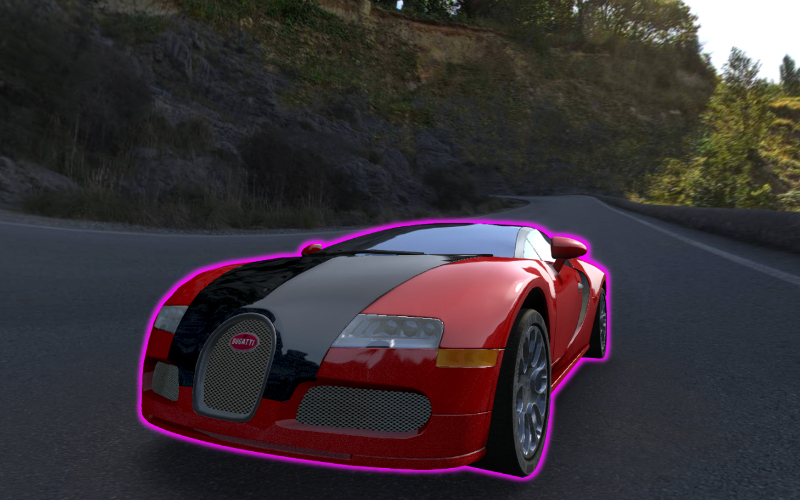
\includegraphics[width=1.000\linewidth]{glow.jpg}\hfill}

\index{anaglyph}\index{stereoscopic rendering}\index{anaglyph}

\section{Stereoscopic rendering (anaglyph)}
\label{postprocessing_effects:anaglyph}\label{postprocessing_effects:index-5}\label{postprocessing_effects:id20}

\subsection{Activation}
\label{postprocessing_effects:id21}
Stereoscopic rendering mode is intended for viewing content using special glasses. It is activated by an application via API.


\subsection{Additional settings}
\label{postprocessing_effects:id22}
No

{\hfill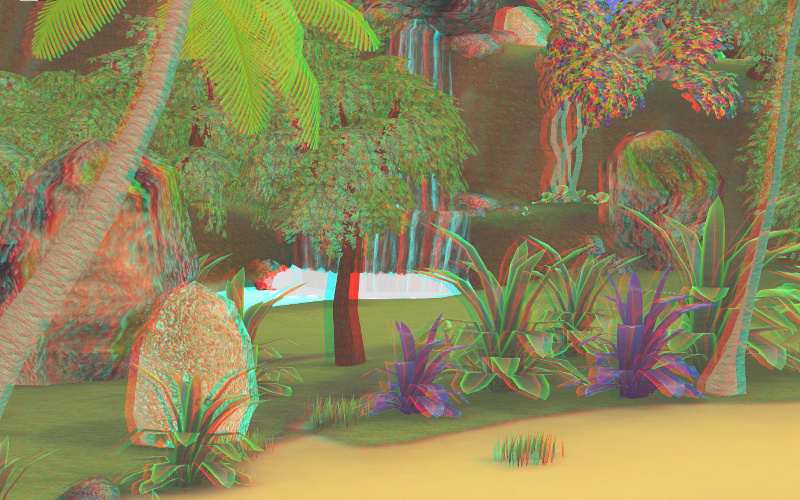
\includegraphics[width=1.000\linewidth]{anaglyph.jpg}\hfill}

\begin{DUlineblock}{0em}
\item[] 
\end{DUlineblock}

\index{color correction}\index{color correction}

\section{Color correction}
\label{postprocessing_effects:index-6}\label{postprocessing_effects:id23}\label{postprocessing_effects:color-correction}

\subsection{Activation}
\label{postprocessing_effects:id24}
Set the \code{Enable Color Correction} checkbox on the \code{Scene \textgreater{} Blend4Web} panel.


\subsection{Additional settings}
\label{postprocessing_effects:id25}
On the \code{World \textgreater{} Blend4Web \textgreater{} Color Correction Settings} panel:
\begin{description}
\item[{\emph{Brightness}}] \leavevmode
The default value is 0.0.

\item[{\emph{Contrast}}] \leavevmode
The default value is 0.0.

\item[{\emph{Exposure}}] \leavevmode
The default value is 1.0.

\item[{\emph{Saturation}}] \leavevmode
The default value is 1.0.

\end{description}

{\hfill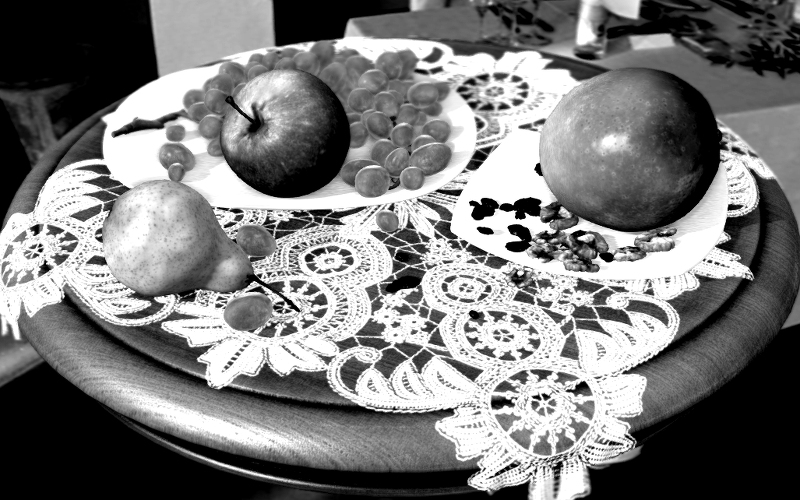
\includegraphics[width=1.000\linewidth]{color_correction.jpg}\hfill}

\begin{DUlineblock}{0em}
\item[] 
\end{DUlineblock}

\index{anti-aliasing}\index{anti-aliasing}

\section{Anti-aliasing}
\label{postprocessing_effects:antialiasing}\label{postprocessing_effects:index-7}\label{postprocessing_effects:id26}
Anti-aliasing is used to reduce undesirable rendering artefacts (poor pixelization).


\subsection{Activation}
\label{postprocessing_effects:id27}
Set the \code{Enable Antialiasing} on the \code{Scene \textgreater{} Blend4Web} panel.


\subsection{Additional settings}
\label{postprocessing_effects:id28}
Anti-aliasing method is assigned simultaneously with selection of the engine performance profile.
\begin{itemize}
\item {} 
\emph{low quality} - anti-aliasing is turned off

\item {} 
\emph{high quality} - anti-aliasing method is FXAA (Fast Approximate Anti-Aliasing) by Nvidia

\item {} 
\emph{maximum quality} - anti-aliasing method is SMAA (Enhanced Subpixel Morphological Anti-Aliasing) by Crytek

\end{itemize}

{\hfill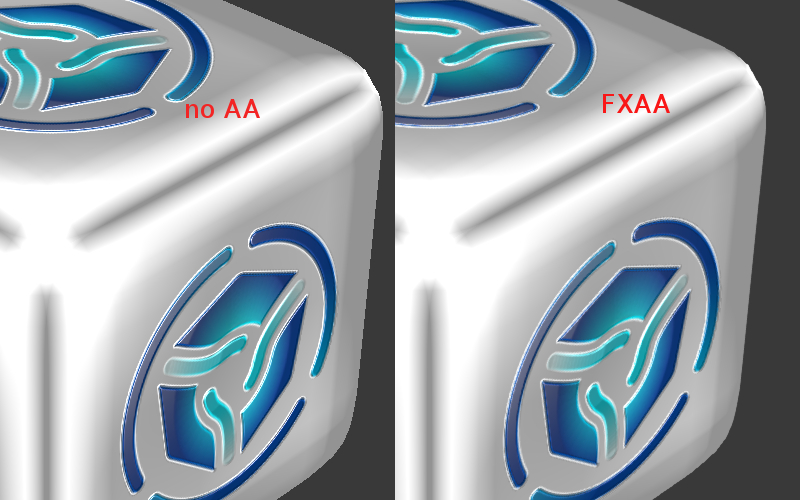
\includegraphics[width=1.000\linewidth]{antialiasing.jpg}\hfill}

\begin{DUlineblock}{0em}
\item[] 
\end{DUlineblock}
\phantomsection\label{particles:particles}
\index{particle system}

\chapter{Particle system}
\label{particles:index-0}\label{particles::doc}\label{particles:id1}
Particle system is intended for visualization of appearances which are caused by numerous small objects movement such as smoke, fire, water splashes and other.

{\hfill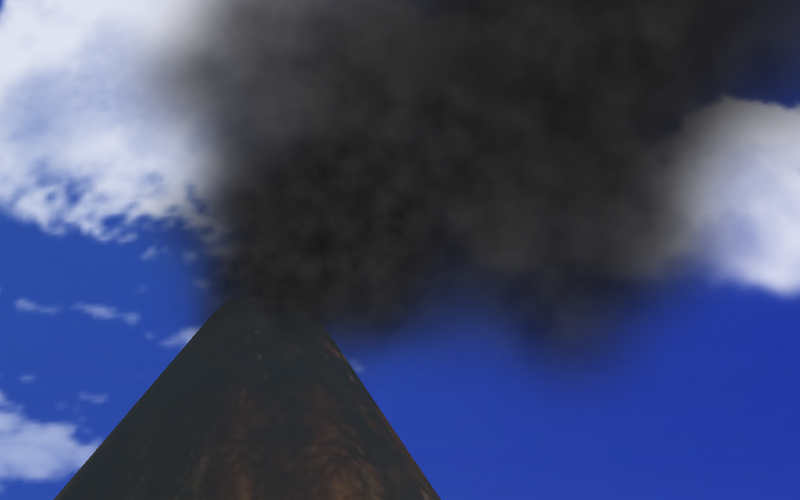
\includegraphics[width=1.000\linewidth]{particles_smoke.jpg}\hfill}

\begin{DUlineblock}{0em}
\item[] 
\end{DUlineblock}

A particle system requires an emitter - an object which defines location and direction of the outgoing particles flow.


\section{Use}
\label{particles:id2}

\subsection{Necessary steps}
\label{particles:id3}\begin{enumerate}
\item {} 
Add a mesh emitter to the scene.

\item {} 
Create a material for particles on the emitter, for example of the \code{Halo} type. Also the \code{Surface} material type with a mandatory diffuse texture is supported.

\item {} 
Add a particle system for the emitter.

\item {} \begin{description}
\item[{Initiate the engine playback. Two options are available:}] \leavevmode\begin{itemize}
\item {} 
``cyclic emission'' - set the \code{Blend4Web \textgreater{} Cyclic emission} checkbox for the particle system.

\item {} 
``non-cyclic animation'' - set the \code{Blend4Web \textgreater{} Animation \textgreater{} Use default} checkbox for the emitter.

\end{itemize}

\end{description}

\end{enumerate}


\subsection{Recommended additional settings}
\label{particles:id4}\begin{enumerate}
\item {} 
Set the \code{Add} transparency type for the particles' material.

\item {} 
Disable emitter rendering if needed using the \code{Particles \textgreater{} Render \textgreater{} Emitter} checkbox.

\item {} 
If an emitter is needed on a scene use additional materials for it. In this case specify the particles' material number (starting from one) in the \code{Particles \textgreater{} Render \textgreater{} Material} field on the particles settings panel.

\item {} 
If the \code{Surface} material type is used it is required to add a diffuse texture (normally with the alpha channel) to this material. Select  \code{UV} in the \code{Mapping \textgreater{} Coordinates} menu.  Make sure that the emitter's mesh has a UV layer.

\end{enumerate}

{\hfill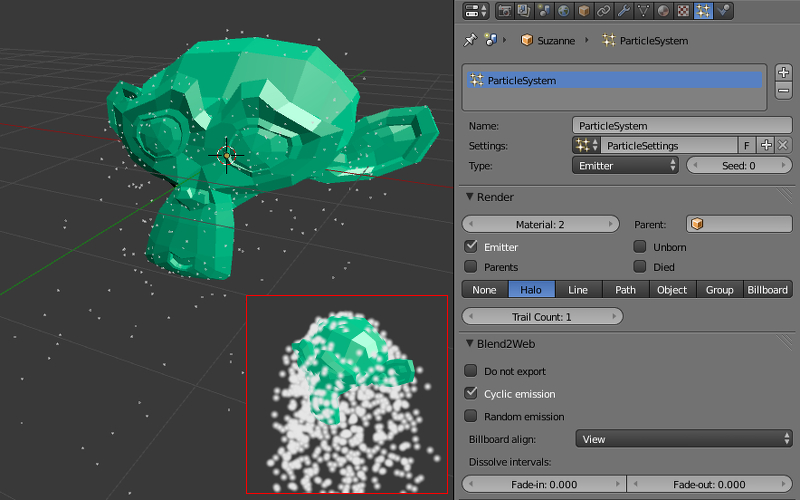
\includegraphics[width=1.000\linewidth]{particles_first_steps.jpg}\hfill}


\section{Setup}
\label{particles:id5}
Particle system parameters can be set up in the \code{Particles} tab. Multiple particle systems per emitter are supported.


\subsection{Basic settings}
\label{particles:id6}\begin{description}
\item[{\emph{Name}}] \leavevmode
Particle system name. The default name is ``ParticleSystem''.

\item[{\emph{Settings}}] \leavevmode
Reference to the settings datablock of the particle system. Settings datablocks can be shared between different particle systems.

\item[{\emph{Type}}] \leavevmode
Particle system type: \code{Emitter} or \code{Hair}. \code{Hair} particle systems can be used for creation of numerous object's copies (so called instancing). The default is \code{Emitter}.

\item[{\emph{Seed}}] \leavevmode
Index in the table of random numbers which are used for particle system generation. The default value is 0.

\end{description}


\subsection{Emission settings}
\label{particles:id7}\begin{description}
\item[{\emph{Emission \textgreater{} Number}}] \leavevmode
Particles count. The default value is 1000.

\item[{\emph{Emission \textgreater{} Start}}] \leavevmode
The first frame after which emission of particles starts. The default value is 1.0.

\item[{\emph{Emission \textgreater{} End}}] \leavevmode
The last frame after which emission of particles ends. The default value is 200.0.

\item[{\emph{Emission \textgreater{} Lifetime}}] \leavevmode
Particles life time measured in frames. The default value is 50.0.

\item[{\emph{Emission \textgreater{} Lifetime \textgreater{} Random}}] \leavevmode
Random factor for life time. The default value is 0.0.

\item[{\emph{Emission \textgreater{} Emit From}}] \leavevmode
Emission source type. The following types are supported: \code{Verts} (emit from vertices), \code{Faces} (emit from polygons). The default is \code{Faces}.

\item[{\emph{Emission \textgreater{} Emit From \textgreater{} Distribution}}] \leavevmode
Emission distribution settings: \code{Jittered}, \code{Random}, \code{Grid}. Ignored by the engine. Internally the engine always uses \code{Random} distribution. The default is \code{Jittered}.

\end{description}

{\hfill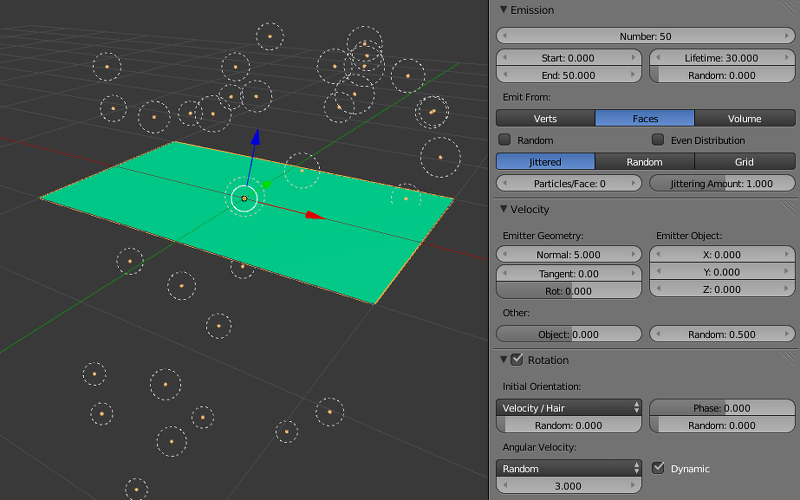
\includegraphics[width=1.000\linewidth]{particles_settings.jpg}\hfill}


\subsection{Direction settings}
\label{particles:id8}
Only the following settings are supported:
\begin{description}
\item[{\emph{Velocity \textgreater{} Emitter Geometry \textgreater{} Normal}}] \leavevmode
Factor of influencing on emission along emitter's mesh normals. The default value is 1.0.

\item[{\emph{Velocity \textgreater{} Other \textgreater{} Random}}] \leavevmode
Factor of randomization for emission direction. The default value is 0.0.

\end{description}


\subsection{Rotation settings}
\label{particles:id9}
Only the following settings are supported:
\begin{description}
\item[{\emph{Rotation \textgreater{} Angular Velocity \textgreater{} Mode}}] \leavevmode
Mode for particle billboards self-rotating. The following modes are supported: \code{Velocity} (constant rotation speed), \code{Random} (random rotation), \code{None} (no rotation). The default is \code{Velocity}.

\item[{\emph{Rotation \textgreater{} Angular Velocity \textgreater{} Factor}}] \leavevmode
Factor of own velocity for particle billboards. The default value is 0.0.

\end{description}


\subsection{Physics settings}
\label{particles:id10}
Only the following settings are supported:
\begin{description}
\item[{\emph{Physics \textgreater{} Type}}] \leavevmode
Physics calculation type: \code{No}, \code{Newtonian}, \code{Keyed}, \code{Boids}, \code{Fluid}. Ignored by the engine. Always the \code{Newtonian} physics is used. The default is \code{Newtonian}.

\item[{\emph{Physics \textgreater{} Size}}] \leavevmode
Particle size. The default value is 0.05.

\item[{\emph{Physics \textgreater{} Mass}}] \leavevmode
Particle mass. Affects interaction with force fields (such as wind). The default value is 1.0.

\item[{\emph{Physics \textgreater{} Forces \textgreater{} Brownian}}] \leavevmode
Exported but not used by the engine.

\end{description}

{\hfill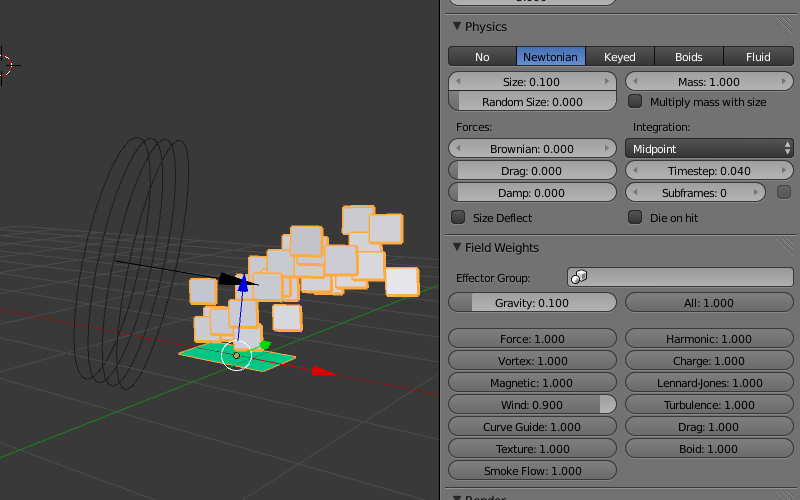
\includegraphics[width=1.000\linewidth]{particles_settings2.jpg}\hfill}


\subsection{Rendering settings}
\label{particles:id11}
Only the following settings are supported:
\begin{description}
\item[{\emph{Render \textgreater{} Material}}] \leavevmode
Material number beginning from one. It is used for referencing to the particles' material in case of multiple materials used by an emitter. The default value is 1.0.

\item[{\emph{Render \textgreater{} Emitter}}] \leavevmode
Enables emitter rendering on a scene. Disabled by default.

\item[{\emph{Render \textgreater{} Type}}] \leavevmode
Particles rendering mode: \code{None}, \code{Halo}, \code{Line}, \code{Path}, \code{Object}, \code{Group}, \code{Billboard}. The engine supports the \code{Object} and the \code{Group} modes which are used for objects and groups instancing respectively. Other modes are ignored. It is recommended to use the \code{Billboard} mode for convenient displaying of billboards. The default is \code{Halo}.

\end{description}


\subsection{Supported settings for force fields influence}
\label{particles:id12}\label{particles:particles-force-fields}
Only the following settings are supported:
\begin{description}
\item[{\emph{Field Weights \textgreater{} Gravity}}] \leavevmode
Influence factor for gravity (Earth's attraction). The default value is 1.0.

\item[{\emph{Field Weights \textgreater{} Wind}}] \leavevmode
Influence factor for wind. A \code{Wind} force field source should present (can be added using \code{Add \textgreater{} Force Field}). A particle system is also influenced by wind direction and strength. The default value is 1.0.

\end{description}


\subsection{Engine specific settings}
\label{particles:id13}\begin{description}
\item[{\emph{Blend4Web \textgreater{} Do not export}}] \leavevmode
Unsupported.

\item[{\emph{Blend4Web \textgreater{} Cyclic emission}}] \leavevmode
Turn on the cyclic mode for emission. It can be used for permanent effects (such as smoke, burning, water splashes). It is recommended to set the \code{Emission \textgreater{} Start} value to zero. Disabled by default.

\item[{\emph{Blend4Web \textgreater{} Random emission}}] \leavevmode
Whether particle emission time is random. Disabled by default.

\item[{\emph{Blend4Web \textgreater{} Billboard align}}] \leavevmode
Billboards orientation mode: \code{View} - rotate to a camera, \code{XY plane}, \code{YZ plane}, \code{ZX plane} - align in the corresponding plane (in the world coordinate system of Blender). The default is \code{View}.

\item[{\emph{Blend4Web \textgreater{} Dissolve intervals \textgreater{} Fade-in} and \emph{Fade-out}}] \leavevmode
Starting and ending intervals (measured in frames) for gradual change of particles' transparency.

\end{description}


\section{Textures in particle systems}
\label{particles:id14}\label{particles:particles-textures}

\subsection{Textures for particles' material}
\label{particles:id15}
For the \code{Surface} particles' materials it is \textbf{required} to have a diffuse texture (normally with the alpha-channel). In the \code{Mapping \textgreater{} Coordinates} menu choose the \code{UV} option.  Make sure that the emitter's mesh has a UV layer.

For the \code{Halo} particles materials it is \textbf{possible} to use a \code{Blend} texture with the \code{Linear} gradient. In the \code{Mapping \textgreater{} Coordinates} menu choose the \code{Strand / Particle} option. It is required to enable \code{Ramp} on a texture. Up to 4 gradient control points are supported.

{\hfill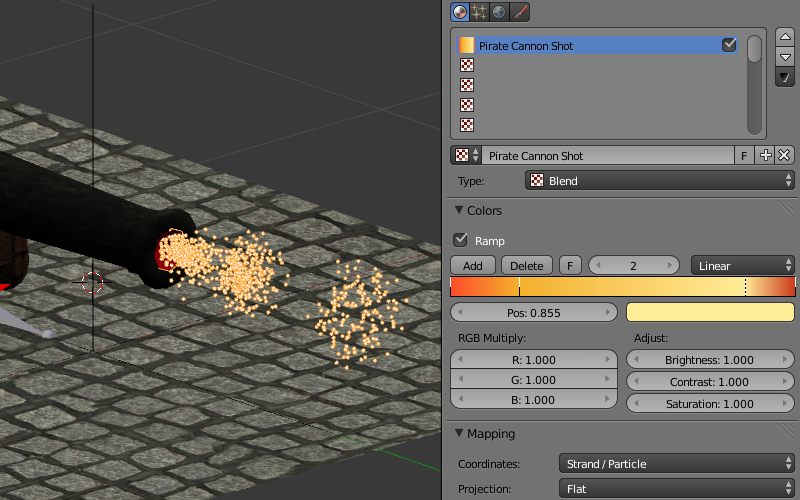
\includegraphics[width=1.000\linewidth]{particles_settings_ramp_color.jpg}\hfill}


\subsection{Textures for particle systems}
\label{particles:id16}
Textures can also be used for particle system behaviour setup. Unlike textures for particles' material such textures belong to a particle system datablock, not to a material datablock. To create a texture for a particle system it is required to go \textbf{from} the \code{Particles} tab to the \code{Textures} tab and then to click the \code{New} button.

\code{Blend} textures with the \code{Linear} gradient are only supported. It is required to enable \code{Ramp} on a texture. Up to 4 gradient control points are supported.

On the \code{Influence} panel it is necessary to choose a parameter which the texture affects. At the moment the only supported parameter is \code{Size}.

{\hfill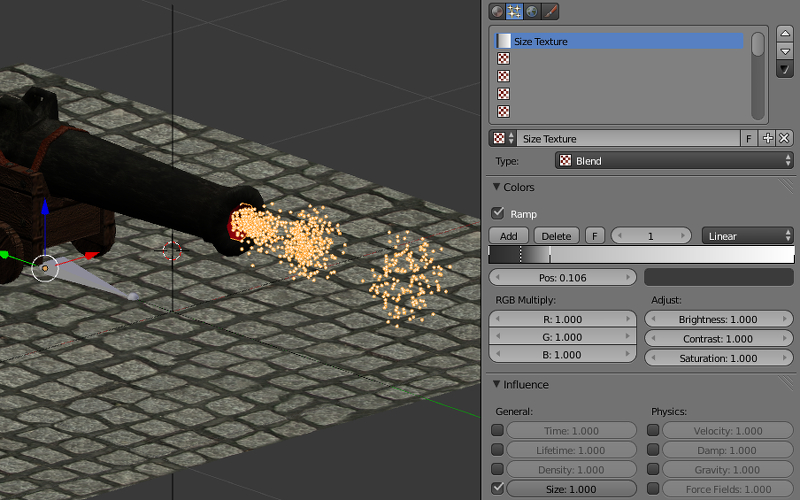
\includegraphics[width=1.000\linewidth]{particles_settings_ramp_size.jpg}\hfill}

\begin{DUlineblock}{0em}
\item[] 
\end{DUlineblock}

Result of using textures for the particles' material and for the particle system:

{\hfill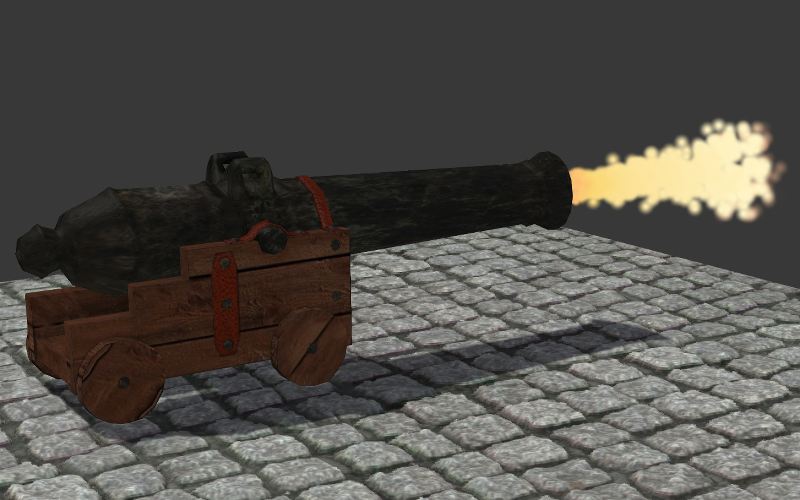
\includegraphics[width=1.000\linewidth]{particles_gun.jpg}\hfill}

\href{http://www.blendswap.com/blends/view/13977}{The original model was taken here}
\phantomsection\label{particles_instancing:particles-instancing}
\index{particle system}\index{instancing}\index{instancing}

\chapter{Particle system for object instancing}
\label{particles_instancing:index-0}\label{particles_instancing::doc}\label{particles_instancing:id1}
A particle system can be used to create multiple object copies (so called instancing).

{\hfill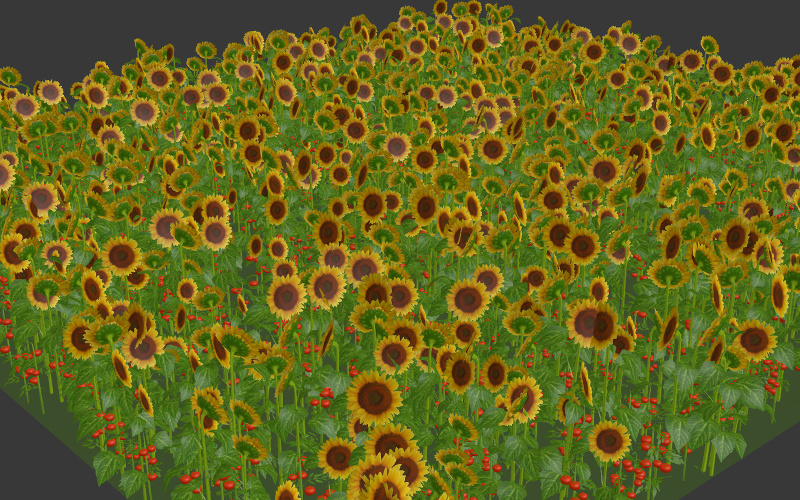
\includegraphics[width=1.000\linewidth]{particles_instancing_example.jpg}\hfill}


\section{Particle system setup}
\label{particles_instancing:id2}
\textbf{Activation}
\begin{enumerate}
\item {} 
Create a particle system of the \code{Hair} type on the emitter.

\item {} 
On the \code{Render} panel select the \code{Object} (or the \code{Group}) rendering type.

\item {} 
In the \code{Dupli Object} field (or in the \code{Dupli Group} field) select the object (or the object group) for instancing. Both local and linked objects (or groups) are supported.

\end{enumerate}

\textbf{Recommended additional settings}
\begin{enumerate}
\item {} 
For correct size displaying set the \code{Emission \textgreater{} Hair Length} and \code{Render \textgreater{} Size} parameters to 1.0.

\item {} 
For correct orientation temporarily enable the \code{Advanced} option, activate the \code{Rotation} panel and select \code{None} in the \code{Initial Orientation} menu. Disable the \code{Advanced} option. It is recommended also to enable the \code{Render \textgreater{} Rotation} option.

\end{enumerate}

{\hfill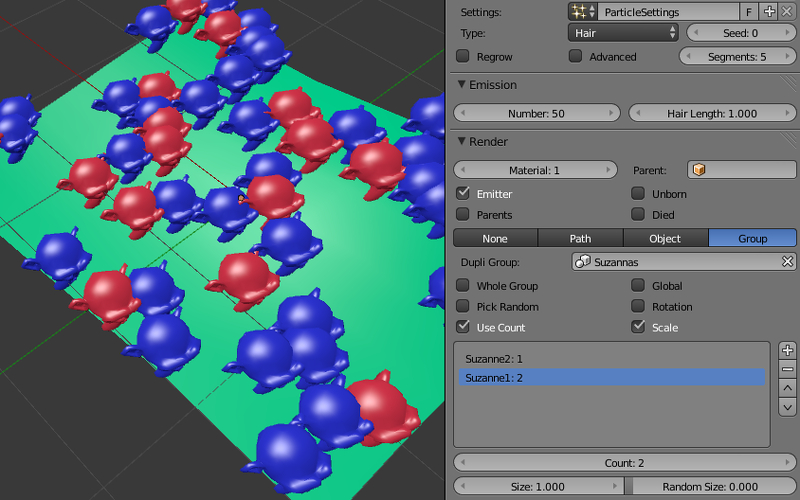
\includegraphics[width=1.000\linewidth]{particles_instancing_setup.jpg}\hfill}

\begin{DUlineblock}{0em}
\item[] 
\end{DUlineblock}

\textbf{Setup}
\begin{description}
\item[{\emph{Render \textgreater{} Use Count}}] \leavevmode
The option is available for groups of particles objects. When enabled the interface for setting the relative number of objects in a group is displayed. The engine doesn't reproduce the exact location for objects of the certain models.

\item[{\emph{Blend4Web \textgreater{} Random location and size}}] \leavevmode
The option enables randomization for the location and the size of the objects. If enabled the engine generates random coordinates and size (limited by the \(\pm\)25\% range) for the particle objects. If it is disabled then the current coordinates and sizes of the particle objects are exported and used. Enabled by default.

\item[{\emph{Blend4Web \textgreater{} Initial random rotation}}] \leavevmode
The option enables randomization for objects' rotation relative to the axis which is defined by the \code{Rotation type} parameter. If enabled the engine generates random rotation angles for the particle objects. If disabled the zero rotation angle is used. Enabled by default.

\item[{\emph{Blend4Web \textgreater{} Rotation type}}] \leavevmode\begin{description}
\item[{The axis for random rotation of the object (the option is available when the \code{Blend4Web \textgreater{} Initial random rotation} checkbox is set). 2 options are available:}] \leavevmode\begin{itemize}
\item {} 
\code{Z axis} - random rotation around the vertical Z axis occurs

\item {} 
\code{Random axis} - random rotation around a random axis occurs

\end{itemize}

\end{description}

The default is \code{Z axis}

\item[{\emph{Blend4Web \textgreater{} Rotation strength}}] \leavevmode\begin{description}
\item[{The coefficient defines range for the random rotation angles - counting out from the camera direction (the option is available when the \code{Blend4Web \textgreater{} Initial random rotation} checkbox is set). Examples:}] \leavevmode\begin{itemize}
\item {} 
\code{Rotation strength = 1} - the angles are in the \([-\pi, \pi]\) range

\item {} 
\code{Rotation strength = 0.5} - the angles are in the \([-0.5 \cdot \pi, 0.5 \cdot \pi]\) range

\item {} 
\code{Rotation strength = 0.1} - the angles are in the \([-0.1 \cdot \pi, 0.1 \cdot \pi]\) range

\end{itemize}

\end{description}

The default value is 1.

\item[{\emph{Blend4Web \textgreater{} Billboard}}] \leavevmode
Enables billboarding for particles. Disabled by default.

\item[{\emph{Blend4Web \textgreater{} Billboard type}}] \leavevmode\begin{description}
\item[{Billboarding type (the option is available when the \code{Blend4Web \textgreater{} Billboard} option is set). The 3 types are available:}] \leavevmode\begin{itemize}
\item {} 
\code{Basic} - simple one-sided billboarding: particles are always turned by front face

\item {} 
\code{Random} - random two-sided billboarding: particles more often turned by front or by back face and less often by side; also there is a small random rotation; this model suits grass instancing well

\item {} 
\code{Jittered} - one-sided billboarding with particles wavering in the plane which is turned to an observer; this model suits tree leaves instancing well

\end{itemize}

\end{description}

The default is \code{Basic}.

\item[{\emph{Blend4Web \textgreater{} Jitter amplitude}}] \leavevmode
Coefficient for particles' oscillation amplitude (the option is available when the \code{Jittered} type is selected from the \code{Blend4Web \textgreater{} Billboard type} menu). The bigger this parameter the bigger the oscillation amplitude. The default value is 0.

\item[{\emph{Blend4Web \textgreater{} Jitter frequency}}] \leavevmode
Particles oscillation frequency in hertz (the option is available when the \code{Jittered} type is selected from the \code{Blend4Web \textgreater{} Billboard type} menu). The default value is 0.

\item[{\emph{Blend4Web \textgreater{} Billboard geometry}}] \leavevmode\begin{description}
\item[{Billboard rotation type (the option is available when the \code{Blend4Web \textgreater{} Billboard} checkbox is set). 2 types are available:}] \leavevmode\begin{itemize}
\item {} 
\code{Spherical} - spherical billboarding i.e. particles are fully oriented to an observer and their rotation is unlimited

\item {} 
\code{Cylindrical} - cylindrical billboarding i.e. particles are rotating only around the vertical Z axis.

\end{itemize}

\end{description}

The default is \code{Spherical}.

\item[{\emph{Blend4Web \textgreater{} Dynamic Grass}}] \leavevmode
The option turns the dynamic grass rendering mode on. Disabled by default.

\item[{\emph{Blend4Web \textgreater{} Wind bending}}] \leavevmode\begin{description}
\item[{Inheriting the wind bending settings by the particles:}] \leavevmode\begin{itemize}
\item {} 
\code{Parent} - inherited from the emitter

\item {} 
\code{Instance} - inherited from the particle object itself

\end{itemize}

\end{description}

The default is \code{Parent}.

\item[{\emph{Blend4Web \textgreater{} Shadows}}] \leavevmode\begin{description}
\item[{Inheriting the shadow settings by particles:}] \leavevmode\begin{itemize}
\item {} 
\code{Parent} - inherited from the emitter

\item {} 
\code{Instance} - inherited from the particle object itself

\end{itemize}

\end{description}

The default is \code{Parent}.

\item[{\emph{Blend4Web \textgreater{} Reflection}}] \leavevmode\begin{description}
\item[{Inheriting the reflection settings by particles:}] \leavevmode\begin{itemize}
\item {} 
\code{Parent} - inherited from the emitter

\item {} 
\code{Instance} - inherited from the particle object itself

\end{itemize}

\end{description}

The default is \code{Parent}.

\item[{\emph{Blend4Web \textgreater{} Vertex color}}] \leavevmode\begin{description}
\item[{Inheriting the vertex color from emitter. Contains 2 fields:}] \leavevmode\begin{itemize}
\item {} 
\code{from} - emitter's existing vertex color name

\item {} 
\code{to} - particle's existing vertex color name

\end{itemize}

\end{description}

There is no inheritance by default.

\end{description}


\section{Grass}
\label{particles_instancing:id3}\label{particles_instancing:particles-grass}
Instancing of objects can be used for visualization of vast grass. In this case grass is rendered near camera when it moves through landscape.

{\hfill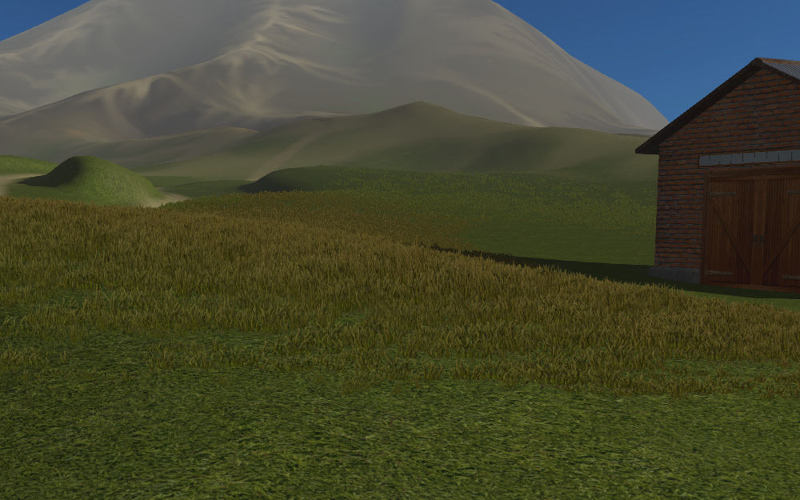
\includegraphics[width=1.000\linewidth]{dynamic_grass.jpg}\hfill}

\begin{DUlineblock}{0em}
\item[] 
\end{DUlineblock}

\textbf{Activation}
\begin{enumerate}
\item {} 
On a separate plane object create a particle system for object instancing. Enable the \code{Blend4Web \textgreater{} Dynamic Grass} option.

\item {} 
On the supposed landscape material enable the \code{Blend4Web \textgreater{} Terrain dynamic grass} option.

\end{enumerate}

\textbf{Setup}

It is recommended to create a few planes (for example 3) with sizes corresponding to the desired grass cascades (e.g. 100, 150 and 250 meters).

On the landscape \textbf{material} the following text fields get active when the \code{Blend4Web \textgreater{} Terrain dynamic grass} option is set:
\begin{description}
\item[{\emph{Dynamic grass size (R)}}] \leavevmode
Vertex color layer name of the landscape mesh which is intended for modifying grass size. The size (i.e. height) of grass is defined by gray tints - the brighter color the higher grass.

\item[{\emph{Dynamic grass color (RGB)}}] \leavevmode
Vertex color layer name of the landscape mesh which is intended for grass tinting. The vertex color is multiplied by the grass material color. The \code{Influence \textgreater{} Blend} parameter forthe grass material's diffuse texture should have the \code{Multiply} value.

\end{description}

Vertex color layers with such names should exist in the landscape mesh.

It is also recommended to disable rendering of the emitter (the \code{Render \textgreater{} Emitter} option).

{\hfill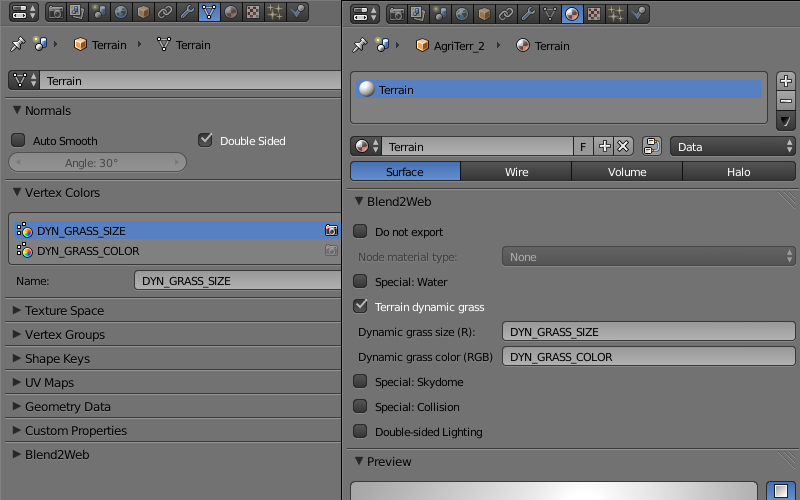
\includegraphics[width=1.000\linewidth]{dynamic_grass_setup.jpg}\hfill}


\section{Tree leaves}
\label{particles_instancing:particles-leaves}\label{particles_instancing:id4}
Instancing suits well to rendering of the tree leaves and allows to get better level of detail.

{\hfill\includegraphics[width=1.000\linewidth]{tree_leaves.jpg}\hfill}

\begin{DUlineblock}{0em}
\item[] 
\end{DUlineblock}

\textbf{Activation}

Is performed as described in the \code{Particle system setup -\textgreater{} Activation} section (see above). In this case a tree is an emitter and leaves and small branches are particles.

Additionally the following operations should be performed for the emitter:
\begin{itemize}
\item {} 
create a vertex group which includes vertices where particles are placed

\item {} 
create a vertex color layer for wind bending parameters of the tree and the leaves

\item {} 
create a vertex color layer to be inherited by particles (for example it can be used for tinting of the particles)

\end{itemize}

\textbf{Setup}
\begin{enumerate}
\item {} 
\code{Random rotation settings}

\end{enumerate}

If the \code{Blend4Web \textgreater{} Initial random rotation} checkbox is set then it is recommended to select the vertical axis for random rotation - \code{Z axis} (the \code{Blend4Web \textgreater{} Rotation type} menu). The \code{Blend4Web \textgreater{} Rotation strength} value can be set too.
\begin{enumerate}
\setcounter{enumi}{1}
\item {} 
\code{Billboarding settings}

\end{enumerate}

It is recommended to enable billboarding, to set its type as \code{Jittered} (the \code{Blend4Web \textgreater{} Billboard type} menu) and to make it spherical - \code{Spherical} (the \code{Blend4Web \textgreater{} Billboard geometry} menu). The \code{Blend4Web \textgreater{} Jitter amplitude} and \code{Blend4Web \textgreater{} Jitter frequency} values can be set too.
\begin{enumerate}
\setcounter{enumi}{2}
\item {} 
\code{Particles location settings}

\end{enumerate}

It is recommended to select the \code{Verts} value from the \code{Emission \textgreater{} Emit From} menu, and to select in the \code{Vertex Group \textgreater{} Density} field an emitter's vertex group which defines placing of particles. Also the \code{Blend4Web \textgreater{} Random location and size} checkbox shoud be disabled.
\begin{enumerate}
\setcounter{enumi}{3}
\item {} 
\code{Wind Bending settings}

\end{enumerate}

It is recommended to enable inheritance settings from the emitter - set the \code{Parent} in the \code{Blend4Web \textgreater{} Wind bending} menu. Then for the emitter on the \code{Object} panel set the \code{Blend4Web \textgreater{} Wind bending} checkbox and setup bending parameters. For a tree it is enough to specify the \code{Blend4Web \textgreater{} Main Bending \textgreater{} Angle} and \code{Blend4Web \textgreater{} Main Bending \textgreater{} Frequency} parameters and also a vertex color name for bending in the \code{Blend4Web \textgreater{} Main Bending \textgreater{} Main stiffness} field.
\begin{enumerate}
\setcounter{enumi}{4}
\item {} 
\code{Vertex color inheritance settings}

\end{enumerate}

For inheritance of the emitter's vertex color it is required to specify the emitter's vertex color name and the particle's vertex color name respectively in the \code{Blend4Web \textgreater{} Vertex Color \textgreater{} from} and \code{Blend4Web \textgreater{} Vertex Color \textgreater{} to} fields. As a result the color of the nearest to the emitter's vertex specified in the \code{from} field will be copied and propagated into the \code{to} particle's vertex color layer.

Resulting vertex color layer with the \code{Blend4Web \textgreater{} Vertex Color \textgreater{} to} name may be used in the particle's node material for its tinting or other effects.

{\hfill\includegraphics[width=1.000\linewidth]{particle_settings.jpg}\hfill}
\phantomsection\label{animation:animation}
\index{animation}\index{animation}

\chapter{Animation}
\label{animation:index-0}\label{animation::doc}\label{animation:id1}
In common case animation is change of any object parameter with time. The engine supports animation of the following types:
\begin{itemize}
\item {} 
Animation of an object as a whole. The parameters that are possible to animate are \code{Location}, \code{Rotation} in the \code{Quaternion(WXYZ)} mode and \code{Scale}.

\item {} 
Skinning (object deformation using bones) and skeletal animation. Animation of a standalone armature object is also supported (for parenting to bones).

\item {} 
Vertex animation - an object deformations can be recorded as frames and then reproduced in the engine.

\item {} 
Audio sources parametrization. Speaker's \code{Volume} and \code{Pitch} can be animated.

\item {} 
Wind bending - a procedural animation. Described {\hyperref[outdoor_rendering:wind]{\emph{separately}}}.

\item {} 
Particle emission. Described in the {\hyperref[particles:particles]{\emph{corresponding section}}}.

\end{itemize}


\section{Animation control}
\label{animation:id2}
Animation can be controlled in the engine in 3 ways:
\begin{enumerate}
\item {} 
Automatically by means of the \code{Animation: Use default} and \code{Animation: Cyclic} checkboxes in an object's properties. In this case an appropriate animation method will be chosen by the engine and the object's animation playback will start just after a scene is loaded.

\item {} 
In an application via API using \code{animation} module methods.

\item {} 
Automatically after editing the \code{assets.json} file of the SDK's viewer. Add  the \code{animated\_objects} property to the scene settings, in which objects' names (or pairs  {[}''empty object name'', ``name of object inside dupli-group''{]}) are listed. This method suits only to applications which use the \code{assets.json} file (right now it is the viewer application from the SDK).

\end{enumerate}

If an object-mesh is animated it is required to set the \code{Do not batch} checkbox on the object properties panel.


\section{Object animation}
\label{animation:id3}
Animation keyframes can be added for an object motion in Blender and then reproduced in the engine.

The following keyframe types are supported:
\begin{itemize}
\item {} 
\emph{Location}

\item {} 
\emph{Rotation} -- the \code{Quaternion(WXYZ)} mode is required.

\item {} 
\emph{Scale} -- for correct results the scale factor should be the same for all 3 axes.

\item {} 
\emph{LocRot} -- a combination of \emph{Location} and \emph{Rotation}.

\item {} 
\emph{LocScale} -- a combination of \emph{Location} and \emph{Scale}.

\item {} 
\emph{LocRotScale} -- a combination of \emph{Location}, \emph{Rotation} and \emph{Scale}.

\item {} 
\emph{RotScale} -- a combination of \emph{Rotation} and \emph{Scale}.

\end{itemize}


\section{Skinning and skeletal animation}
\label{animation:id4}
For skeletal animation both a mesh object and an armature object are needed. The 4 steps should be carried out:
\begin{enumerate}
\item {} 
Create the object's ``skeleton'' in the armature object.

\item {} 
Assign vertex groups in the mesh object and link them to the the bones. This can be performed by weight painting for example.

\item {} 
Animate the bones in the pose mode of the armature object. The same keyframe types can be used as for object animation.

\item {} 
When inverse kinematics (IK) or other nontrivial structures are used - bake actions for the engine using the \code{B4W Animation Bake} operator which can be executed via search box (\code{SPACE}).

\end{enumerate}


\section{Vertex animation}
\label{animation:id5}
Allows to record any geometry changes of a mesh object. Note that every vertex animation frame count as mesh. Don't make long animation for a high-poly mesh.

Special tool is used for baking vertex animation - \code{B4W Vertex Anim Baker} - located on the \code{Blend4Web} tools panel.


\section{Audio source parametrization}
\label{animation:id6}
In addition on speaker objects the following animation key types are supported:
\begin{itemize}
\item {} 
\emph{Volume}

\item {} 
\emph{Pitch}

\end{itemize}


\chapter{Outdoor Rendering}
\label{outdoor_rendering:outdoor-rendering}\label{outdoor_rendering::doc}\label{outdoor_rendering:id1}

\section{Water}
\label{outdoor_rendering:id2}

\subsection{Activation}
\label{outdoor_rendering:id3}
For the supposed water material enable the \code{Blend4Web \textgreater{} Special: Water} option in the \code{Material} tab.

{\hfill\includegraphics[width=1.000\linewidth]{water_material_setup.jpg}\hfill}


\subsection{Basic settings}
\label{outdoor_rendering:id4}\begin{description}
\item[{\emph{Transparency}}] \leavevmode
It is recommended to enable a gradient transparency \code{Game Settings \textgreater{} Alpha Blend} and to tweak the \code{Transparency \textgreater{} Alpha} value.

\item[{\emph{Lighting parameters}}] \leavevmode
Lighting parameters for the water material can be set up as described in the {\hyperref[materials:material-lighting-params]{\emph{Lighting parameters}}} section.

\end{description}


\subsection{Waves dynamics}
\label{outdoor_rendering:id5}
Waves simulation is carried out by normal maps with animated UVs (from 0 up to 4 pieces). For normal textures the only one shared image is used - the textures differ only by the \code{Mapping \textgreater{} Size} and \code{Blend4Web \textgreater{} UV translation velocity} parameters. The water mesh should have a UV layer.
\begin{figure}[htbp]
\centering

\includegraphics[width=0.700\linewidth]{water_texture_setup_normal.jpg}
\end{figure}


\subsection{Surface wetting}
\label{outdoor_rendering:id6}
Carried out automatically. To enable the effect set the \code{Wettable} checkbox on the needed materials.


\subsection{Reflection and Fresnel effect}
\label{outdoor_rendering:id7}
For the water material both static and dynamic reflection is supported as well as the Fresnel effect. See the {\hyperref[materials:material-mirror]{\emph{Reflection}}} section.

{\hfill\includegraphics[width=1.000\linewidth]{water_reflection_dynamic.jpg}\hfill}


\subsection{Shore smoothing}
\label{outdoor_rendering:id8}\begin{description}
\item[{\emph{Blend4Web \textgreater{} Water Settings \textgreater{} Shore smoothing}}] \leavevmode
Enable smoothing.

\item[{\emph{Blend4Web \textgreater{} Water Settings \textgreater{} Water absorb factor}}] \leavevmode
Light absorption coefficient for water. The higher it the more transparent water.

\end{description}

In the low quality mode an {\hyperref[textures:texture-alpha-map]{\emph{alpha map}}} can be used instead of this option.


\subsection{Color gradient}
\label{outdoor_rendering:id9}
For color gradient the water material should have a texture with the \code{Blend4Web \textgreater{} Shore distance map} option enabled which can be generated using the script for {\hyperref[outdoor_rendering:shore-distance-bake]{\emph{shore parameters baking}}}.
\begin{description}
\item[{\emph{Blend4Web \textgreater{} Water Settings \textgreater{} Shallow water color}}] \leavevmode
Shallow water color.

\item[{\emph{Blend4Web \textgreater{} Water Settings \textgreater{} Shallow water color factor}}] \leavevmode
Factor for mixing shallow water color.

\item[{\emph{Blend4Web \textgreater{} Water Settings \textgreater{} Shore water color}}] \leavevmode
Water color just near the shore line.

\item[{\emph{Blend4Web \textgreater{} Water Settings \textgreater{} Shore water color factor}}] \leavevmode
Factor for mixing water color just near the shore line.

\end{description}


\subsection{Refraction}
\label{outdoor_rendering:id10}
In the \code{Scene} tab enable the \code{Blend4Web \textgreater{} Render refractions} option.

{\hfill\includegraphics[width=1.000\linewidth]{water_refraction.jpg}\hfill}


\subsection{Foam}
\label{outdoor_rendering:id11}

\subsubsection{Activation}
\label{outdoor_rendering:id12}
For creating foam add two diffuse textures into the water material slots. For these textures enable the \code{Blend4Web \textgreater{} Water Foam} option.
\begin{figure}[htbp]
\centering

\scalebox{0.700000}{\includegraphics{water_texture_setup_foam.jpg}}
\end{figure}


\subsubsection{The textures setup}
\label{outdoor_rendering:id13}\begin{description}
\item[{\emph{Influence \textgreater{} Color}}] \leavevmode
Influence of texture color. The default value is 1.0.

\item[{\emph{Blend4Web \textgreater{} UV Frequency}}] \leavevmode
Oscillation frequency of the animated UV coordinates. The default value is (1.0, 1.0).

\item[{\emph{Blend4Web \textgreater{} UV Magnitude}}] \leavevmode
Oscillation amplitude of the animated UV coordinates. The default value is (1.0, 1.0).

\end{description}


\subsubsection{The material setup}
\label{outdoor_rendering:id14}\begin{description}
\item[{\emph{Blend4Web \textgreater{} Water Settings \textgreater{} Water foam factor}}] \leavevmode
General influence factor for the foam. The default value is 0.5.

\end{description}


\subsection{Caustics and chromatic aberration}
\label{outdoor_rendering:id15}
To create the caustics effect add one \code{Voronoi} type texture to the water material slot.

{\hfill\includegraphics[width=1.000\linewidth]{water_caustics.jpg}\hfill}


\subsubsection{Setup}
\label{outdoor_rendering:id16}\begin{figure}[htbp]
\centering

\scalebox{0.800000}{\includegraphics{water_texture_setup_caustics.jpg}}
\end{figure}
\begin{description}
\item[{\emph{Voronoi \textgreater{} Coloring: Intensity}}] \leavevmode
Caustics influence factor. The default value is 1.0.

\item[{\emph{Voronoi \textgreater{} Noise: Size}}] \leavevmode
Cell size for the procedural texture. The default value is 0.25.

\item[{\emph{Blend4Web \textgreater{} UV translation velocity}}] \leavevmode
Texture coordinates animation speed. The default value is (0.0, 0.0).

\end{description}


\subsection{Underwater environment}
\label{outdoor_rendering:id17}
{\hfill\includegraphics[width=1.000\linewidth]{underwater.jpg}\hfill}


\subsubsection{Visibility settings (``fog'')}
\label{outdoor_rendering:id18}\begin{description}
\item[{\emph{Blend4Web \textgreater{} Water Settings \textgreater{} Underwater fog density}}] \leavevmode
Exponential factor which affects density and visibility distance. The default value is 0.06.

\item[{\emph{Blend4Web \textgreater{} Water Settings \textgreater{} Underwater fog color}}] \leavevmode
Fog color. The default value is (0.5, 0.5, 0.5) (gray).

\end{description}

The {\hyperref[postprocessing_effects:god-rays]{\emph{god rays effect}}} settings are also applied.


\subsection{Boundary between environments}
\label{outdoor_rendering:id19}
Disable the \code{Game Settings \textgreater{} Backface Culling} option.

{\hfill\includegraphics[width=1.000\linewidth]{water_border.jpg}\hfill}


\subsection{Volumetric waves}
\label{outdoor_rendering:id20}\label{outdoor_rendering:water-volumetric-waves}

\subsubsection{Activation}
\label{outdoor_rendering:id21}
\emph{Blend4Web \textgreater{} Water Settings \textgreater{} Water Dynamic}

Enable volumetric waves.

{\hfill\includegraphics[width=1.000\linewidth]{water_waves.jpg}\hfill}


\subsubsection{Setup}
\label{outdoor_rendering:id22}\begin{description}
\item[{\emph{Blend4Web \textgreater{} Water Settings \textgreater{} Wave height}}] \leavevmode
Wave height. The default value is 0.0.

\item[{\emph{Blend4Web \textgreater{} Water Settings \textgreater{} Wave length}}] \leavevmode
Wave length. The default value is 10.0.

\item[{\emph{Blend4Web \textgreater{} Water Settings \textgreater{} Dist noise scale 0}}] \leavevmode
Size of the first component for distant waves.

\item[{\emph{Blend4Web \textgreater{} Water Settings \textgreater{} Dist noise scale 1}}] \leavevmode
Size of the second component for distant waves.

\item[{\emph{Blend4Web \textgreater{} Water Settings \textgreater{} Dist noise freq 0}}] \leavevmode
Frequency of the first component for distant waves.

\item[{\emph{Blend4Web \textgreater{} Water Settings \textgreater{} Dist noise freq 1}}] \leavevmode
Frequency of the second component for distant waves.

\item[{\emph{Blend4Web \textgreater{} Water Settings \textgreater{} Dir min shore fac}}] \leavevmode
Minimum coefficient for decreasing height of waves near shore.

\item[{\emph{Blend4Web \textgreater{} Water Settings \textgreater{} Dir frequency}}] \leavevmode
Frequency of waves rolling near shore.

\item[{\emph{Blend4Web \textgreater{} Water Settings \textgreater{} Dir noise scale}}] \leavevmode
Noise size for waves near shore.

\item[{\emph{Blend4Web \textgreater{} Water Settings \textgreater{} Dir noise freq}}] \leavevmode
Noise frequency for waves near shore.

\item[{\emph{Blend4Web \textgreater{} Water Settings \textgreater{} Dir min noise fac}}] \leavevmode
Noise minimum for waves near shore.

\item[{\emph{Blend4Web \textgreater{} Water Settings \textgreater{} Dist min fac}}] \leavevmode
Minimum coefficient for mixing distant waves.

\item[{\emph{Blend4Web \textgreater{} Water Settings \textgreater{} Waves horizontal factor}}] \leavevmode
Coefficient for shifting waves near shore to the shore direction.

\end{description}


\subsection{Generated surface settings}
\label{outdoor_rendering:id23}\begin{description}
\item[{\emph{Blend4Web \textgreater{} Water Settings \textgreater{} Generate mesh}}] \leavevmode
Enable generated surface.

\item[{\emph{Blend4Web \textgreater{} Water Settings \textgreater{} Number of cascades}}] \leavevmode
Number of cascades in generated surface.

\item[{\emph{Blend4Web \textgreater{} Water Settings \textgreater{} Detailed distance}}] \leavevmode
Maximum distance from camera to the last cascade edge.

\end{description}

\index{shore line parameters}\index{shore line}

\subsubsection{Creating texture with shore line parameters.}
\label{outdoor_rendering:index-0}\label{outdoor_rendering:id24}\label{outdoor_rendering:shore-distance-bake}
On the tools panel (hotkey ``T'') under the \code{Blend4Web} tab open the \code{B4W Shore Distance Baker} panel. Set the parameters: maximum distance to shore (\code{Maximum Distance}) and resulting texture size (\code{Texture Size}). Select a landscape object first (or multiple objects), and then a water object. Click the \code{Bake Shore Distance} button.

Depending on texture size and vertices number in processing meshes the execution time of the script may vary from a fraction of a second up to several minutes. Make sure the texture named \code{ShoreDistance} is created for the water mesh.

Upon script execution some system properties are saved in the water material. Therefore the scene after script run must be saved.


\section{Atmosphere}
\label{outdoor_rendering:id25}

\subsection{Scattering}
\label{outdoor_rendering:id26}
Create a plane object for skydome as specified in the {\hyperref[textures:skydome-texture]{\emph{Skydome}}} section. Environment map is not needed. Set the \code{Special: Skydome} and \code{Procedural skydome} options on the material.

{\hfill\includegraphics[width=1.000\linewidth]{skydome_procedural.jpg}\hfill}

\begin{DUlineblock}{0em}
\item[] 
\end{DUlineblock}

The settings are located under the \code{World} tab.
\begin{description}
\item[{\emph{Sky Settings \textgreater{} Sky color}}] \leavevmode
Base sky color. The default value is (0.087, 0.255, 0.6) (blue).

\item[{\emph{Sky Settings \textgreater{} Rayleigh brightness}}] \leavevmode
Rayleigh scattering brightness (i.e. scattering on small particles). The default value is 3.3.

\item[{\emph{Sky Settings \textgreater{} Mie brightness}}] \leavevmode
Mie scattering brightness (i.e. scattering on large particles). The default value is 0.1.

\item[{\emph{Sky Settings \textgreater{} Spot brightness}}] \leavevmode
Sun spot brightness. The default value is 20.0.

\item[{\emph{Sky Settings \textgreater{} Scatter strength}}] \leavevmode
Light scattering factor. The default value is 0.2.

\item[{\emph{Sky Settings \textgreater{} Rayleigh strength}}] \leavevmode
Rayleigh scattering factor. The default value is 0.2.

\item[{\emph{Sky Settings \textgreater{} Mie strength}}] \leavevmode
Mie scattering factor. The default value is 0.006.

\item[{\emph{Sky Settings \textgreater{} Rayleigh collection power}}] \leavevmode
Rayleigh scattering exponent. The default value is 0.35.

\item[{\emph{Sky Settings \textgreater{} Mie collection power}}] \leavevmode
Mie scattering exponent. The default value is 0.5.

\item[{\emph{Sky Settings \textgreater{} Mie distribution}}] \leavevmode
Mie scattering distribution. The default value is 0.4.

\end{description}


\subsection{Fog}
\label{outdoor_rendering:id27}
Can be set up under the \code{World} tab.
\begin{description}
\item[{\emph{Blend4Web \textgreater{} Fog Settings \textgreater{} Fog density}}] \leavevmode
Exponential factor which affects density and visibility distance. The default value is 0.0.

\item[{\emph{Blend4Web \textgreater{} Fog Settings \textgreater{} Fog color}}] \leavevmode
Fog color. The default value is (0.5, 0.5, 0.5) (gray).

\end{description}

When dynamic skydome is used a fog color is defined by sky color.


\subsection{Time of day}
\label{outdoor_rendering:id28}
Enable the \code{Blend4Web \textgreater{} Dynamic intensity} option for a lamp.

Time of day can be set by applications via API. Particularly time of day can be set using the \code{Lighting} interface of the {\hyperref[viewer:viewer]{\emph{Scene viewer}}}.

{\hfill\includegraphics[width=1.000\linewidth]{sunset.jpg}\hfill}


\subsection{Stars}
\label{outdoor_rendering:id29}
Stars setup is described in the {\hyperref[materials:material-halo]{\emph{Halo materials}}} section.

{\hfill\includegraphics[width=1.000\linewidth]{stars.jpg}\hfill}


\section{Wind}
\label{outdoor_rendering:id30}\label{outdoor_rendering:wind}\begin{description}
\item[{Wind strength and direction affect}] \leavevmode\begin{itemize}
\item {} 
{\hyperref[outdoor_rendering:wind-bending]{\emph{grass and tree leaves animation}}}

\item {} 
{\hyperref[particles:particles-force-fields]{\emph{particle system dynamics}}}

\item {} 
{\hyperref[outdoor_rendering:water-volumetric-waves]{\emph{water waves rolling frequency}}} (at the moment only strength is taken into account)

\end{itemize}

\end{description}


\subsection{Activation}
\label{outdoor_rendering:id31}
Add a force field object of the \code{Wind} type.


\subsection{Setup}
\label{outdoor_rendering:id32}\begin{description}
\item[{\emph{Direction}}] \leavevmode
Direction can be set by rotating the force field object.

\item[{\emph{Force Fields \textgreater{} Strength}}] \leavevmode
Wind strength. Located under the \code{Physics} tab. The default value is 1.0.

\end{description}


\subsection{Grass and tree leaves animation}
\label{outdoor_rendering:wind-bending}\label{outdoor_rendering:id33}
Authoring resources for grass rendering is described in the {\hyperref[particles_instancing:particles-grass]{\emph{Grass}}} section.


\subsubsection{Activation}
\label{outdoor_rendering:id34}
Enable the \code{Blend4Web \textgreater{} Wind bending} option for the grass or tree object.


\subsubsection{Setup}
\label{outdoor_rendering:id35}
The interface panel becomes visible after activation of the \code{Blend4Web \textgreater{} Wind bending} option.

{\hfill\includegraphics[width=1.000\linewidth]{wind_bending_setup.jpg}\hfill}

\begin{DUlineblock}{0em}
\item[] 
\end{DUlineblock}
\begin{description}
\item[{\emph{Main bending \textgreater{} Angle}}] \leavevmode
Angle amplitude of the ``main'' deviation under the influence of wind (in degrees). The default value is 10.0.

\item[{\emph{Main bending \textgreater{} Frequency}}] \leavevmode
Frequency of the ``main'' deviation under the influence of wind. The default value is 0.25.

\item[{\emph{Main bending \textgreater{} Main stiffness (A)}}] \leavevmode
Text field for specifing name of a vertex color layer which contains information about stiffness of the ``main'' deviation. Can be left empty.

\item[{\emph{Detail bending \textgreater{} Detail amplitude}}] \leavevmode
Angle amplitude of the ``detail'' deviation under the influence of wind (in degrees). The default value is 0.1.

\item[{\emph{Detail bending \textgreater{} Branch amplitude}}] \leavevmode
Angle amplitude of the branch deviation under the influence of wind (in degrees). The default value is 0.3.

\item[{\emph{Detail bending \textgreater{} Leaves stiffness (R)}}] \leavevmode
Text field for specifing name of a vertex color layer which contains information about stiffness of leaves. Can be left empty.

\item[{\emph{Detail bending \textgreater{} Leaves phase (G)}}] \leavevmode
Text field for specifing name of a vertex color layer which contains information about phase of leaves deviation. Can be left empty.

\item[{\emph{Detail bending \textgreater{} Overall stiffness (B)}}] \leavevmode
Text field for specifing name of a vertex color layer which contains information about overall stiffness of leaves. Can be left empty.

\end{description}

Vertex color layers should exist in the mesh if their names are specified.

{\hfill\includegraphics[width=1.000\linewidth]{wind_bending_vcolors.jpg}\hfill}


\chapter{Gamma-correction and transparency}
\label{gamma_alpha::doc}\label{gamma_alpha:gamma}\label{gamma_alpha:id1}

\section{Общее описание}
\label{gamma_alpha:id2}
Сущность гамма-коррекции заключается в упаковке яркости канала изображения в 8
битах информации. Особенности восприятия человеческого глаза и технические
характеристики электронно-лучевых трубок имеют вторичное значение.

Графические редакторы обычно работают в нелинейном цветовом пространстве,
где тёмные компоненты кодируются большим числом битов чем светлые. Это означает,
что значению 0.5 от реальной интенсивности света (физической величины, называемой
освещённость) будет соответствовать большее значение каналов RGB (в самом
простом случае 0.5 \textasciicircum{} (1/2.2) = 0.73).

{\hfill\includegraphics[width=1.000\linewidth]{gamma.jpg}\hfill}

\begin{DUlineblock}{0em}
\item[] 
\end{DUlineblock}

Изображения всегда сохраняются в нелинейном пространстве, в противном случае 8
бит информации не достаточно для кодирования интенсивности света, что приведёт к
тому, что тёмные тона будут отображаться некорректно.

Веб-браузеры работают в нелинейном пространстве.

Blender при настройке сцены \code{Color Managment \textgreater{} Display Device \textgreater{} sRGB} работает в линейном
пространстве. Значения цветов материалов и настройки источников света
соответствует физическим величинам. При работе с текстурами, за исключением карт
нормалей необходимо выставить настройку изображения \code{Image \textgreater{} Input Color Space \textgreater{} sRGB}.
В этом случае при рендеринге будет производится автоматическая распаковка
изображения: sRGB-\textgreater{}Linear.

Движки и рендереры работают в линейном пространстве, поскольку только оно может
адекватно представлять поведение света в реальном мире. Если взять две
одинаковые лампочки и включать их последовательно, освещённость от воздействия
обеих будет ровно в два раза превышать освещённость только от одной.

Примеры величин освещённости:

\begin{tabulary}{\linewidth}{|L|L|}
\hline
\textsf{\relax 
Описание
} & \textsf{\relax 
Освещённость,лк
}\\
\hline
Летом в полдень
 & 
17 000
\\

Зимой в полдень
 & 
5 000
\\

В пасмурный день
 & 
1 000
\\

В светлой комнате
 & 
100
\\

Ночью в полнолуние
 & 
0.2
\\

В безлунную ночь
 & 
0.001
\\
\hline\end{tabulary}



\section{Человеческое зрение, ЭЛТ-мониторы}
\label{gamma_alpha:id3}
Человеческое восприятие света нелинейно (человек лучше различает градации
тусклого света чем яркого), однако свет, поступающий в глаз,
по-прежнему должен подчиняться физическим законам (см. пример с лампочками).

ЭЛТ-мониторы имеют нелинейную характеристику яркости от приложенного к их входу
электрического напряжения (чаще всего определяется непосредственно значением
канала цветности в видеопамяти), подобную же характеристику копируют мониторы,
основанные на других технологиях. Однако свет, излучаемый такими мониторами,
должен подчиняться физическим законам. В идеальном случае при добавлении второго
источника света на сцену в виртуальном мире, яркость пикселей на экране монитора
должна увеличиваться в два раза.


\section{Гамма}
\label{gamma_alpha:id4}
Используется в формуле:
\begin{quote}

V$_{\text{out}}$ = V$_{\text{in}}$$^{\text{\(\gamma\)}}$
\end{quote}

\(\gamma\) \textless{} 1 - упаковывающая гамма, \(\gamma\) \textgreater{} 1 - распаковывающая гамма. В наиболее простом
случае используются значения 1/2.2 и 2.2 соответственно. Далее вместо термина
``гамма-коррекция'' будут использованы термины ``упаковка'' и ``распаковка''. Сильно
упрощая, под упаковкой понимается преобразование Linear-\textgreater{}sRGB, под распаковкой
sRGB-\textgreater{}Linear.


\section{Коррекция в нодовых материалах}
\label{gamma_alpha:gamma-nodes}\label{gamma_alpha:id5}
При использовании текстур и вертексных цветов в качестве источников цвета,
необходима распаковка (sRGB-\textgreater{}Linear). Нода текстуры уже включает в себя
распаковку, в то время как для вертексного цвета необходимо использовать ноду
\emph{SRGB\_TO\_LINEAR}.

При использовании карт нормалей никакие преобразования не производятся.

При использовании текстур и вертексных цветов в качестве масок для смешения
цветов или других математических операций в преобразованиях нет необходимости.
Однако в этом случае следует обратить внимание на то, как происходит
преобразование цветов при сохранении изображений в графических редакторах. В
большинстве случаев значения, выставленные в редакторе, попадают в изображения без
изменений. Иногда возможна небольшая коррекция, которая не будет
иметь существенного влияния на итоговый результат.

Как было сказано ранее, ноды текстуры включают в себя распаковку. Это приводит к
необходимости двойного преобразования обратно в нелинейное пространство, для
чего используется нода \emph{LINEAR\_TO\_SRGB}.

Сводная таблица коррекции в нодовых материалах:

\begin{tabulary}{\linewidth}{|L|L|}
\hline
\textsf{\relax 
Случай использования
} & \textsf{\relax 
Коррекция
}\\
\hline
Текстура для окраски
 & 
встроена в ноду текстуры
\\

Вертексный цвет для окраски
 & 
SRGB\_TO\_LINEAR
\\

Карта нормалей
 & 
не требуется
\\

Текстура для маски
 & 
LINEAR\_TO\_SRGB
\\

Вертексный цвет для маски
 & 
не требуется
\\
\hline\end{tabulary}



\section{Альфа-композитинг}
\label{gamma_alpha:id6}
Физически корректный альфа-композитинг осуществляется по формуле:
\begin{quote}

\(C_o = C_a \alpha_a + C_b \alpha_b (1 - \alpha_a)\).
\end{quote}

Формула отличается от классической операции смешивания (mix, выпуклая комбинация) наличием множителя \(\alpha_b\) во втором слагаемом. То есть, для осуществления альфа-композитинга, необходимо знать не только альфу пикселя-источника, то и альфу пикселя, поверх которого осуществляется рендеринг.

В случае предварительного умножения значений альфы на цветовые каналы (т.н.
Premultiplied Alpha):
\begin{quote}

\(C_o = C_a + C_b (1 - \alpha_a)\).
\end{quote}

Последняя формула используется также для расчёта результирующей альфы:
\begin{quote}

\(\alpha_o = \alpha_a + \alpha_b (1 - \alpha_a)\).
\end{quote}

Предварительное умножение цветовых каналов на значение альфы позволяет сэкономить две операции умножения, однако более существенным является тот факт, что полученная формула может использоваться многократно, без необходимости деления исходного пикселя на значение альфы на каждой последующей итерации.

Таким образом, функция смешивания WebGL должна иметь вид:

\begin{Verbatim}[commandchars=\\\{\}]
gl.blendFunc(gl.ONE, gl.ONE\PYGZus{}MINUS\PYGZus{}SRC\PYGZus{}ALPHA);
\end{Verbatim}

Инициализация контекста должна производиться с параметром \emph{premultipliedAlpha : true}. Кроме того, необходимо обеспечить правильный рендеринг прозрачных материалов на выходе шейдера, для чего используется умножение всех каналов цветности на значение альфы.


\chapter{Звуковая подсистема}
\label{audio:audio}\label{audio::doc}\label{audio:id1}
Создание звуковых источников осуществляется в Blender'e. Используется стандартный объект \code{Speaker}.


\section{Настройка звуковых источников}
\label{audio:id2}
Настройки спикера выставляются в панели \code{Properties} на вкладке \code{Object Data}.
\begin{description}
\item[{\emph{Speaker behavior}}] \leavevmode
Поведение звукового источника.

\code{Positional} --- высококачественный звук, допускающий позиционирование и
имеющий направленность (конусность). Для рендеринга используется Web Audio
API. Воспроизведение подобных звуков обладает наименьшей производительностью,
поэтому их использовать целесообразно только для коротких сэмплов.

\code{Background sound} --- высококачественный всенаправленный звук без возможности
позиционирования в пространстве. Для рендеринга используется Web Audio API.
Более производителен, однако нецелесообразен для музыки.

\code{Background music} --- используется для воспроизведения музыки. Максимальная
производительность вследствие использования тега Audio, минимальная гибкость.

\item[{\emph{Disable doppler}}] \leavevmode
Игнорировать смещение частоты источника при его перемещении.

\item[{\emph{Cyclic play}}] \leavevmode
Зацикливать воспроизведение звука.

\item[{\emph{Delay}}] \leavevmode
Задержка в секундах перед началом проигрывания звука.

\item[{\emph{Random delay}}] \leavevmode
Дополнительная рандомизация задержки, результирующее значение определяется
по формуле \(Delay_{result} = Delay + Delay_{random} * Random_{[0-1]}\).

\item[{\emph{Random volume}}] \leavevmode
Дополнительная рандомизация громкости. Результирующее значение определяется
аналогично задержке.

\item[{\emph{Random pitch}}] \leavevmode
Дополнительная рандомизация скорости проигрывания звука. Результирующее значение определяется
аналогично задержке.

\item[{\emph{Fade-in}}] \leavevmode
Интервал плавного включения звука.

\item[{\emph{Fade-out}}] \leavevmode
Интервал плавного выключения звука.

\item[{\emph{Loop}}] \leavevmode
Зацикливать воспроизведение звука. Отличается от \code{Cyclic play},
тем, что способен обеспечить нулевую задержку при повторении. Опция доступна
только для звуковых источников с поведением \code{Positional} или \code{Background
sound}.

\item[{\emph{Loop count}}] \leavevmode
Не реализовано

\item[{\emph{Random loop count}}] \leavevmode
Не реализовано

\item[{\emph{Playlist ID}}] \leavevmode
Не реализовано

\end{description}


\section{Обработка и кодирование}
\label{audio:id3}\label{audio:encoding}

\subsection{Поддерживаемые форматы (контейнеры):}
\label{audio:id4}\begin{itemize}
\item {} 
ogg, кодек Vorbis (Chrome, Firefox)

\item {} 
mp3 (Chrome, Safari)

\item {} 
mp4, кодек AAC (Chrome, Safari)

\end{itemize}

Рекомендуется использовать ogg, как наиболее распространённый в браузерах,
поддерживающих WebGL (Chrome, Firefox). Оптимальным с точки зрения качества и
совместимости является формат 48кГц/16. Одноканальный звук (моно) используется
для хранения коротких сэмплов, двухканальный звук (стерео) - для музыкального
сопровождения.

Встроенный конвертер имеет возможность преобразования исходных форматов для
расширения спектра поддерживаемых платформ. Для этого необходимо выполнить
команду:

\begin{Verbatim}[commandchars=\\\{\}]
\PYGZgt{} ./converter.py convert\PYGZus{}sounds
\end{Verbatim}

Преобразование происходит по схеме:
\begin{itemize}
\item {} 
ogg -\textgreater{} mp4

\item {} 
mp3 -\textgreater{} ogg

\item {} 
mp4 -\textgreater{} ogg

\end{itemize}

Конвертация ресурсов происходит с потерей качества, поэтому сконвертированные
файлы получают суффикс .lossconv.


\chapter{Событийная модель}
\label{event_model:id1}\label{event_model::doc}\label{event_model:event-model}
Событийная модель предоставляет унифицированный интерфейс для описания
изменения состояний 3D сцены, упрощая обработку событий физики и действий
пользователя.

\index{сенсор}\index{sensor}

\section{Сенсоры}
\label{event_model:id2}\label{event_model:index-0}
Основным блоком событийной модели является сенсор (sensor). Сенсор является
программной сущностью, и может быть только активным (1, единица) или неактивным (0, ноль).
Некоторые сенсоры несут полезную нагрузку (payload). Например, сенсор трассировки лучей (Ray Sensor)
предоставляет относительную длину луча пересечения.

\index{сенсор!множество}\index{sensor!manifold}
Управление сенсорами не доступно пользователю в виде открытого API. Вместо этого
каждый сенсор должен присутствовать в одном или нескольких множествах (sensor
manifold). Множество является логическим контейнером, ассоциированным с объектом на сцене.
Оно определяет ответ на групповое событие сенсоров в виде вызова
функции-обработчика. Для определения множества необходимо иметь
следующую информацию (см. функцию \code{b4w.controls.create\_sensor\_manifold()}).
\begin{itemize}
\item {} 
Объект-носитель множества (например, объект персонажа).

\item {} 
Уникальный идентификатор множества (например, ``JUMP'').

\item {} \begin{description}
\item[{Тип вызова функции-обработчика (варианты: \code{CT\_CONTINUOUS} - непрерывный,}] \leavevmode
\code{CT\_LEVEL} - уровень, \code{CT\_SHOT} - одномоментный, \code{CT\_TRIGGER} - переключающий).

\end{description}

\item {} 
Массив сенсоров.

\item {} 
Логическая функция, определяющая при каких состояниях сенсоров будет
вызываться функция-обработчик.

\item {} 
Функция обработчик.

\item {} 
Необязательный параметр, который может быть передан в функцию-обработчик.

\end{itemize}

Например, стоит задача определить взаимодействие некоторого бросаемого
физического объекта с окружающими предметами. Причём при ударе о различные
объекты должен выводиться характерный звук. В простом случае определяется один
сенсор соударения (Collision Sensor) для каждого объекта из окружения. Сенсоры
добавляются в множества по типу издаваемого звука. В качестве логической функции
здесь выступает логическое ИЛИ. В обработчике пишется код для воспроизведения
звука:

\begin{Verbatim}[commandchars=\\\{\}]
\PYG{c+c1}{// array of sensors}
\PYG{k+kd}{var} \PYG{n+nx}{metal\PYGZus{}sens\PYGZus{}array} \PYG{o}{=} \PYG{p}{[}\PYG{n+nx}{sensor\PYGZus{}iron}\PYG{p}{,} \PYG{n+nx}{sensor\PYGZus{}copper}\PYG{p}{]}\PYG{p}{;}

\PYG{c+c1}{// manifold logic callback}
\PYG{k+kd}{var} \PYG{n+nx}{metal\PYGZus{}sens\PYGZus{}logic} \PYG{o}{=} \PYG{k+kd}{function}\PYG{p}{(}\PYG{n+nx}{s}\PYG{p}{)} \PYG{p}{\PYGZob{}}\PYG{k}{return} \PYG{p}{(}\PYG{n+nx}{s}\PYG{p}{[}\PYG{l+m+mi}{0}\PYG{p}{]} \PYG{o}{\textbar{}\textbar{}} \PYG{n+nx}{s}\PYG{p}{[}\PYG{l+m+mi}{1}\PYG{p}{]}\PYG{p}{)}\PYG{p}{\PYGZcb{}}\PYG{p}{;}

\PYG{c+c1}{// callback}
\PYG{k+kd}{var} \PYG{n+nx}{metal\PYGZus{}cb} \PYG{o}{=} \PYG{k+kd}{function}\PYG{p}{(}\PYG{n+nx}{obj}\PYG{p}{,} \PYG{n+nx}{id}\PYG{p}{,} \PYG{n+nx}{value}\PYG{p}{,} \PYG{n+nx}{pulse}\PYG{p}{)} \PYG{p}{\PYGZob{}}
    \PYG{c+c1}{// play sound here}
\PYG{p}{\PYGZcb{}}
\PYG{c+c1}{// create manifold}
\PYG{n+nx}{m\PYGZus{}ctl}\PYG{p}{.}\PYG{n+nx}{create\PYGZus{}sensor\PYGZus{}manifold}\PYG{p}{(}\PYG{n+nx}{throwing\PYGZus{}object}\PYG{p}{,} \PYG{l+s+s2}{\PYGZdq{}METAL\PYGZus{}COLLISION\PYGZdq{}}\PYG{p}{,} \PYG{n+nx}{m\PYGZus{}ctl}\PYG{p}{.}\PYG{n+nx}{CT\PYGZus{}SHOT}\PYG{p}{,}
        \PYG{n+nx}{metal\PYGZus{}sens\PYGZus{}array}\PYG{p}{,} \PYG{n+nx}{metal\PYGZus{}sens\PYGZus{}logic}\PYG{p}{,} \PYG{n+nx}{metal\PYGZus{}cb}\PYG{p}{)}\PYG{p}{;}
\end{Verbatim}


\chapter{Физика}
\label{physics:physics}\label{physics::doc}\label{physics:id1}

\section{Подготовка к использованию}
\label{physics:id2}
Физическая подсистема реализована в независимо загружающемся модуле uranium.js, содержащем портированный на JavaScript физический движок Bullet. Для установки использования физической подсистемы и пути загрузки модуля uranium.js приложения должны использовать API:

\begin{Verbatim}[commandchars=\\\{\}]
\PYG{n+nx}{b4w}\PYG{p}{.}\PYG{n+nx}{config}\PYG{p}{.}\PYG{n+nx}{set}\PYG{p}{(}\PYG{l+s+s2}{\PYGZdq{}physics\PYGZus{}enabled\PYGZdq{}}\PYG{p}{,} \PYG{k+kc}{true}\PYG{p}{)}\PYG{p}{;}
\PYG{n+nx}{b4w}\PYG{p}{.}\PYG{n+nx}{config}\PYG{p}{.}\PYG{n+nx}{set}\PYG{p}{(}\PYG{l+s+s2}{\PYGZdq{}physics\PYGZus{}uranium\PYGZus{}path\PYGZdq{}}\PYG{p}{,} \PYG{l+s+s2}{\PYGZdq{}../../external/deploy/apps/common/uranium.js\PYGZdq{}}\PYG{p}{)}\PYG{p}{;}
\end{Verbatim}

Для задействования физики на сцене необходимо установить флаг \code{Enable physics} в интерфейсе сцены.

\includegraphics[width=1.000\linewidth]{scene.jpg}

\begin{DUlineblock}{0em}
\item[] 
\end{DUlineblock}

Настройка физических параметров производится в режиме \code{Blender Game}.

\includegraphics[width=1.000\linewidth]{info_panel.jpg}

\begin{DUlineblock}{0em}
\item[] 
\end{DUlineblock}


\section{Статический меш}
\label{physics:id3}
Может использоваться как ограничитель движения других объектов, например, для определения столкновений с ландшафтом, стенами и т.д. В настройках физики такого объекта для опции \code{Physics Type} должно быть выбрано значение \code{Static} (значение по умолчанию).
\begin{figure}[htbp]
\centering

\includegraphics[width=0.800\linewidth]{physics_panel_static.jpg}
\end{figure}

\begin{DUlineblock}{0em}
\item[] 
\end{DUlineblock}

Меш может быть покрыт одним или несколькими физическими материалами. В панели материала должен быть установлен флаг \code{Special: Collision}. Среди физических настроек материала поддерживаются: трение (\code{Friction}), упругость (\code{Elasticity}).

\includegraphics[width=1.000\linewidth]{material_panel_physics.jpg}

\begin{DUlineblock}{0em}
\item[] 
\end{DUlineblock}

Поле \code{Collision ID} предназначено для определения столкновения со специфическим материалом, и может быть оставлено пустым. Пример использования \code{Collision ID} - определение нахождения игрового персонажа на разных типах покрытия ландшафта - трава, песок, деревянное покрытие и т.д.

Опция \code{Ghost} исключает материал из физических взаимодействий, но сообщает приложению о контакте с ним. Пример - определение, что игровой персонаж находится на вертикальной лестнице.

\includegraphics[width=1.000\linewidth]{physics_water_tower.jpg}

\begin{DUlineblock}{0em}
\item[] 
\end{DUlineblock}

Поле \code{Collision group} отвечает за физическую группу, к которой относится материал.
Поле \code{Collision mask} определяет все физические группы, с которыми будет взаимодействовать данный материал.


\section{Динамический объект}
\label{physics:id4}
Предназначен для симуляции движения жесткого тела.

\includegraphics[width=1.000\linewidth]{physics_dynamic.jpg}

\begin{DUlineblock}{0em}
\item[] 
\end{DUlineblock}

В настройках физики такого объекта для опции \code{Physics Type} может быть выбрано значение \code{Rigid Body} (с вращениями) или \code{Dynamic} (без вращений). В настройках \code{Collision Bounds} может быть выбран тип коллайдера, поддерживаются: \code{Box}, \code{Capsule}, \code{Sphere}, \code{Cylinder}, \code{Cone}. Другие поддерживаемые настройки: масса (\code{Mass}), демпфирование (\code{Damping}) - для перемещения (\code{Translation}) и вращения (\code{Rotation}).

Поле \code{Collision group} отвечает за физическую группу, к которой относится объект.

Поле \code{Collision mask} определяет все физические группы, с которыми будет взаимодействовать данный объект.
\begin{figure}[htbp]
\centering

\includegraphics[width=0.800\linewidth]{physics_panel_dynamic.jpg}
\end{figure}

\begin{DUlineblock}{0em}
\item[] 
\end{DUlineblock}

В настройках панели физики объекта должен быть установлен флаг \code{Detect collisions}. Поле \code{Collision ID} предназначено для определения столкновения со специфическим объектом (например, прикрепленный к камере объект для определения близости FPS персонажа к предметам), и может быть оставлено пустым.
\begin{figure}[htbp]
\centering

\includegraphics[width=0.800\linewidth]{object.jpg}
\end{figure}

\begin{DUlineblock}{0em}
\item[] 
\end{DUlineblock}

Для материала динамического объекта поддерживаются: трение (\code{Friction}), упругость (\code{Elasticity}). В случае использования на одном меше нескольких материалов физические настройки считываются с первого из них.

Для объекта-камеры должна использоваться настройка \code{Physics Type} = \code{Dynamic}, должен быть установлен флаг \code{Detect collisions}.


\section{Ограничители (Constraints)}
\label{physics:constraints}
Физические ограничители используются для уменьшения числа степеней свободы объектов.

\includegraphics[width=1.000\linewidth]{physics_constraints.jpg}

\begin{DUlineblock}{0em}
\item[] 
\end{DUlineblock}

Установка физического ограничителя (\code{Rigid Body Joint}) на объект происходит в панели \code{Object Constraints}. Поддерживаемые типы (\code{Pivot Type}): \code{Ball}, \code{Hinge}, \code{Cone Twist}, \code{Generic 6 DoF}. Физический ограничитель можно установить на один из двух взаимодействующих объектов, при этом другой выступает в качестве цели (\code{Target}). Оба объекта могут быть статическими и/или динамическими. В ограничителях (кроме \code{Ball}) могут настраиваться пределы перемещения и вращения.

\includegraphics[width=1.000\linewidth]{physics_constraints_panel.jpg}

\begin{DUlineblock}{0em}
\item[] 
\end{DUlineblock}


\section{Колесные транспортные средства}
\label{physics:id5}
Модель транспортного средства (ТС) должна состоять из 6 отдельных объектов - шасси, 4 колеса, рулевое колесо. Центр меша шасси должен соответсвовать центру масс. Центры мешей колес и рулевого колеса должны располагаться на осях вращения. Рулевое колесо должно быть ориентировано в локальной системе координат: X - ось вращения, Y - вправо, Z - вверх. Объекты могут иметь любые названия.

\includegraphics[width=1.000\linewidth]{physics_vehicle_wheeled.jpg}

\begin{DUlineblock}{0em}
\item[] 
\end{DUlineblock}

На всех 6 объектах нужно выставить \code{Vehicle part}, указать один и тот же идентификатор в поле \code{Vehicle name}, выбрать соответствующий тип объекта - \code{Chassis}, \code{Steering wheel}, \code{Back right wheel} и т.д. Для колес имеется также настройка компенсирующего хода подвески \code{Suspension rest length}.

Для шасси необходимо указать реалистичную массу (т.к. значение по умолчанию 1 кг). Для этого перейти в настройки физики, для опции \code{Physics Type} выбрать значение \code{Rigid Body}, и выставить нужное значение (например, 1000 кг) в поле \code{Mass}.


\subsection{Параметры настройки для шасси}
\label{physics:id6}\begin{description}
\item[{\emph{Vehicle Settings \textgreater{} Force max}}] \leavevmode
Максимальная движущая сила транспортного средства

\item[{\emph{Vehicle Settings \textgreater{} Brake max}}] \leavevmode
Максимальный коэффициент торможения

\item[{\emph{Vehicle Settings \textgreater{} Suspension compression}}] \leavevmode
Коэффициент демпфирования при растяжении подвески

\item[{\emph{Vehicle Settings \textgreater{} Suspension stiffness}}] \leavevmode
Коэффициент жесткости подвески

\item[{\emph{Vehicle Settings \textgreater{} Suspension damping}}] \leavevmode
Коэффициент амортизации подвески

\item[{\emph{Vehicle Settings \textgreater{} Wheel friction}}] \leavevmode
Константа трения колес о поверхность. Для реалистичных Т.С. должен быть в районе 0.8. Но может быть значительно увеличен, для улучшения управляемости (1000 и более)

\item[{\emph{Vehicle Settings \textgreater{} Roll influence}}] \leavevmode
Снижает вращающий момент от колес, уменьшая вероятность переворота транспортного средства (0 - нет вращающего момента, 1 - реальное физическое поведение)

\item[{\emph{Vehicle Settings \textgreater{} Max suspension travel cm}}] \leavevmode
Максимальный ход подвески в сантиметрах

\end{description}

Для рулевого колеса(\code{Steering wheel}) необходимо указать максимальный угол поворота(\code{Steering max}) и передаточное отношение угла поворота руля к
передним колесам (\code{Steering ratio}). Максимальное значение угла поворота укзывается в оборотах. Один оборот равен 360 градусам. Таким образом,
поставив \code{Steering max} равным единице, а \code{Steering ratio} равным 10, максимальный поворот руля получится равным 360 градусав, а максимальный
поворот передних колес 36 градусов.

На этом этапе можно произвести экспорт и загрузить сцену в движок. Рекомендуется создать дорожную поверхность с физическим материалом. В просмотрщике нажать клавишу \code{Q} для установки контролируемого объекта, и выбрать шасси. Использовать \code{W}, \code{A}, \code{S}, \code{D} для управления.

Дополнительно можно настроить демпфирование \code{Damping} перемещения (\code{Translation}) и вращения (\code{Rotation}). Свойство влияет на скорость перемещения и инерционность ТС.

Настройка трения и эластичности физического материала дорожного покрытия не влияют на поведение ТС.


\section{Плавающие объекты}
\label{physics:id7}
\includegraphics[width=1.000\linewidth]{physics_floater.jpg}

\begin{DUlineblock}{0em}
\item[] 
\end{DUlineblock}

Для того, чтобы объект мог плавать на поверхности воды (объекта с материалом \code{Special water}), необходимо выставить свойство \code{Floating}. Существует два типа частей плавающего объекта: \code{Main body} - непосредственно сам плавающий объект и \code{Bob} - вспомогательный объект-поплавок, на который будет действовать выталкивающая из воды сила. Плавающий объект может иметь неограниченное количество объектов типа \code{Bob}. В качестве поплавков могут использоваться как меши, так и объекты типа \code{Empty}.

Всем объектам, входящим в состав одного плавающего объекта необходимо выставить одинаковое имя в поле \code{Floater name}


\subsection{Параметры настройки плавающего объекта}
\label{physics:id8}\begin{description}
\item[{\emph{Floating settings \textgreater{} Floating factor}}] \leavevmode
Коэффициент выталкивания объекта из воды

\item[{\emph{Floating settings \textgreater{} Water linear damping}}] \leavevmode
Демпфирование линейной скорости при нахождении отбъекта на поверхности воды (или под водой). Когда объект находится вне воды, используется значение из настроек физики.

\item[{\emph{Floating settings \textgreater{} Water rotation damping}}] \leavevmode
Демпфирование вращения при нахождении отбъекта на поверхности воды (или под водой). Когда объект находится вне воды, используется значение из настроек физики.

\end{description}


\section{Плавающие транспортные средства}
\label{physics:id9}
\includegraphics[width=1.000\linewidth]{physics_boat.jpg}

\begin{DUlineblock}{0em}
\item[] 
\end{DUlineblock}

Плавающие транспортные средства используют часть параметров из настроек \code{Vehicle settings} и все настройки аналогичные \code{Floating settings}. На основном объекте необходимо выставить \code{Vehicle part}, типа \code{Hull}. Так же как и плавающий объект плавающее транспортное средство требует наличия вспомогательных объектов типа \code{Bob}.


\subsection{Параметры настройки плавающего транспортного средства}
\label{physics:id10}\begin{description}
\item[{\emph{Vehicle Settings \textgreater{} Force max}}] \leavevmode
Максимальная движущая сила транспортного средства

\item[{\emph{Vehicle Settings \textgreater{} Brake max}}] \leavevmode
Максимальный коэффициент торможения

\item[{\emph{Floating settings \textgreater{} Floating factor}}] \leavevmode
Коэффициент выталкивания объекта из воды

\item[{\emph{Floating settings \textgreater{} Water linear damping}}] \leavevmode
Демпфирование линейной скорости при нахождении отбъекта на поверхности воды (или под водой). Когда объект находится вне воды, используется значение из настроек физики.

\item[{\emph{Floating settings \textgreater{} Water rotation damping}}] \leavevmode
Демпфирование вращения при нахождении отбъекта на поверхности воды (или под водой). Когда объект находится вне воды, используется значение из настроек физики.

\end{description}


\chapter{Методики создания ресурсов}
\label{assets_creation::doc}\label{assets_creation:id1}

\section{Карты нормалей}
\label{assets_creation:normal-mapping}\label{assets_creation:id2}
Качество 3D-моделей напрямую зависит от уровня ее детализации. С ростом числа полигонов возрастает объем данных, время их загрузки и обработки, уменьшается скорость отрисовки. С целью обхода указанных ограничений применяется метод изготовления карт нормалей. Смысл метода заключается в создании высокополигональной модели, детализация которой затем переносится (``запекается'') на основную низкополигональную модель в виде специальной текстуры (карты нормалей).

{\hfill\includegraphics[width=1.000\linewidth]{normals_1.png}\hfill}

Пример высокополигональной модели и полученной на ее основе низкополигональной.


\subsection{Что такое ``нормали''}
\label{assets_creation:id3}
Нормаль - перпендекуляр к поверхности - имеет важное значение для расчета освещения. При отображении 3D-объекта в графическом движке происходит сравнение нормали в каждой точке с направлением падения света. В результате поверхность, нормаль которой находится по одну сторону с направлением света, отображается как освещенная (если наоборот - то как затемненная).

{\hfill\includegraphics[width=1.000\linewidth]{normals_2.png}\hfill}

Ориентация нормалей на поверхности трехмерного объекта.


\subsection{Что такое ``карта нормалей''}
\label{assets_creation:id4}
Для реализации освещения (без карты нормалей) графический движок использует нормали, рассчитанные в каждой точке меша - т.е. для каждого вертекса. Для отображения пикселов, расположенных между вертексами, используются усредненные нормали. Карта нормалей позволяет использовать ``точные'', указанные художником, нормали вместо усредненных.

{\hfill\includegraphics[width=1.000\linewidth]{normals_3.png}\hfill}

Затенение объекта без карты нормалей.

{\hfill\includegraphics[width=1.000\linewidth]{normals_4.png}\hfill}

Карта нормалей полученная с высокополигонального объекта.

{\hfill\includegraphics[width=1.000\linewidth]{normals_5.png}\hfill}

Затенение объекта c картой нормалей.


\chapter{Проблемы и решения}
\label{problems_and_solutions:problems-and-solutions}\label{problems_and_solutions::doc}\label{problems_and_solutions:id1}

\section{Инициализация WebGL}
\label{problems_and_solutions:webgl}\label{problems_and_solutions:webgl-not-working}
Сайт \href{http://get.webgl.org/}{http://get.webgl.org/} при просмотре в браузерах Chrome или Firefox последней версии сообщает о проблемах. Что делать?

\textbf{На Windows}:
\begin{enumerate}
\item {} 
Установить доступные \href{http://support.microsoft.com/kb/311047/ru}{обновления} для системы. Установить последнюю версию \href{http://www.microsoft.com/downloads/ru-ru/details.aspx?FamilyID=2da43d38-db71-4c1b-bc6a-9b6652cd92a3\&displayLang=ru}{DirectX}. Перезагрузить систему.

\item {} 
В некоторых случаях может понадобиться установка драйверов от производителей графических карт. Чтобы определить тип и производителя карты, можно воспользоваться средством диагностики DirectX...

\end{enumerate}

{\hfill\includegraphics[width=1.000\linewidth]{dxdiag.jpg}\hfill}

или ввести about:gpu в адресную строку браузера Chrome.

{\hfill\includegraphics[width=1.000\linewidth]{about_gpu_directx.jpg}\hfill}

Необходимо загрузить драйверы с соответствующего центра поддержки (например, \href{http://downloadcenter.intel.com/Default.aspx?lang=rus}{Intel}, \href{http://www.nvidia.com/Download/index.aspx?lang=ru}{Nvidia}, \href{http://support.amd.com/us/gpudownload/Pages/index.aspx}{AMD/ATI}). После установки драйверов перезагрузить систему.
\begin{enumerate}
\setcounter{enumi}{2}
\item {} 
Если в результате вышеперечисленных действий инициализировать рендеринг не удается (или нет возможности обновить систему), можно попробовать изменить настройки браузера.

\end{enumerate}

\emph{В Chrome}:

Ввести about:flags в адресную строку браузера, нажать \code{Включить} (\code{Enable}) под опцией \code{Переопределение списка программного рендеринга} (\code{Override software rendering list}) и перезапустить браузер.

{\hfill\includegraphics[width=1.000\linewidth]{about_flags_force_webgl.jpg}\hfill}

\emph{В Firefox}:

Ввести about:config в адресную строку браузера, найти параметр \code{webgl.force-enabled} и переключить его двойным щелчком мыши из \code{false} в \code{true}.

{\hfill\includegraphics[width=1.000\linewidth]{about_config_force_webgl.jpg}\hfill}

\textbf{На Linux}:
\begin{enumerate}
\item {} 
Ввиду неполной реализации OpenGL стека в драйверах с открытым кодом в настоящий момент рекомендуется использовать проприетарные драйверы текущей версии для графических процессоров Nvidia и AMD.

\item {} 
Форсирование графической акселерации из п. 3 для Windows происходит аналогично для Chrome. В случае Firefox предлагается использовать переменную окружения:

\begin{Verbatim}[commandchars=\\\{\}]
\PYGZgt{} MOZ\PYGZus{}GLX\PYGZus{}IGNORE\PYGZus{}BLACKLIST=1 firefox
\end{Verbatim}

\end{enumerate}


\section{Настройка браузера для загрузки локальных ресурсов}
\label{problems_and_solutions:browser-for-local-loading}\label{problems_and_solutions:id3}
Движок является Web-приложением, и его работа происходит при просмотре html-файла в браузере. После инициализации происходит загрузка ресурсов (сцен, текстур), которая подчиняется \href{http://ru.wikipedia.org/wiki/Правило\_ограничения\_домена}{правилу ограничения домена}, запрещающему, в частности, загрузку из локальной директории. Простым способом обхода этого ограничения может быть настройка браузера (рекомендуется). Другой способ заключается в использовании {\hyperref[problems_and_solutions:local-web-server]{\emph{локального web-сервера}}}.

\begin{notice}{note}{Note:}
Рекомендуется использовать такой браузер только для просмотра локального контента, поскольку изменение настроек может привести к понижению безопасности.
\end{notice}

\emph{Chrome на Windows}:

Правой кнопкой мыши нажать на ярлыке на рабочем столе, выбрать \code{Свойства} (\code{Properties}), после чего в поле для пути к исполняемому файлу добавить после пробела \code{-{-}allow-file-access-from-files}. Нажать \code{ОК}.

{\hfill\includegraphics[width=1.000\linewidth]{chrome_file_access.jpg}\hfill}

Для удобства можно предварительно создать копию ярлыка и изменить ее для локального просмотра, оставив оригинальную версию ярлыка для запуска браузера в обычном режиме.

\emph{Chrome/Chromium на Linux}:

Запустить браузер с параметром:

\begin{Verbatim}[commandchars=\\\{\}]
\PYGZgt{} google\PYGZhy{}chrome \PYGZhy{}\PYGZhy{}allow\PYGZhy{}file\PYGZhy{}access\PYGZhy{}from\PYGZhy{}files
\end{Verbatim}

или:

\begin{Verbatim}[commandchars=\\\{\}]
\PYGZgt{} chromium\PYGZhy{}browser \PYGZhy{}\PYGZhy{}allow\PYGZhy{}file\PYGZhy{}access\PYGZhy{}from\PYGZhy{}files
\end{Verbatim}

\emph{Firefox на Windows/Linux}:

Ввести about:config в адресную строку браузера, найти параметр \code{security.fileuri.strict\_origin\_policy} и переключить его двойным щелчком мыши из \code{true} в \code{false}.

{\hfill\includegraphics[width=1.000\linewidth]{firefox_strict_origin.jpg}\hfill}


\section{Использование локального web-сервера}
\label{problems_and_solutions:local-web-server}\label{problems_and_solutions:web}
Простым вариантом может быть запуск web-сервера из стандартной библиотеки \href{http://ru.wikipedia.org/wiki/Python}{Python}.

\emph{На Windows}:
\begin{enumerate}
\item {} 
Загрузить и инсталлировать последнюю версию Python с \href{http://www.python.org/download/releases/}{официального сайта}. На сегодняшний день это версия 3.2, и по умолчанию установка произойдет в директорию \code{Python32} на диске \code{C}.

\item {} 
Запустить командную строку (Command Prompt).

\item {} 
Выполнить команды:

\begin{Verbatim}[commandchars=\\\{\}]
\PYGZgt{} c:
\PYGZgt{} /Python32/python \PYGZhy{}m http.server
\end{Verbatim}

\item {} 
Перейти на страницу \href{http://localhost:8000}{http://localhost:8000}, на которой выбрать нужный файл для отображения.

\end{enumerate}

\emph{На Linux}:

\begin{Verbatim}[commandchars=\\\{\}]
\PYGZgt{} python \PYGZhy{}m SimpleHTTPServer
\end{Verbatim}

или:

\begin{Verbatim}[commandchars=\\\{\}]
\PYGZgt{} python3 \PYGZhy{}m http.server
\end{Verbatim}

Можно указать порт дополнительным параметром:

\begin{Verbatim}[commandchars=\\\{\}]
\PYGZgt{} python \PYGZhy{}m SimpleHTTPServer 8080
\end{Verbatim}


\section{Проблемы при запуске рендерера}
\label{problems_and_solutions:id6}\label{problems_and_solutions:renderer-not-working}
\emph{1. Появляется сообщение ``browser not supported''.}

Браузер не поддерживается.

\emph{2. Появляется сообщение ``underlying error''.}

Следует выполнить действия, описанные в разделе {\hyperref[problems_and_solutions:webgl-not-working]{\emph{Инициализация WebGL}}}.

\emph{3. Видны элементы интерфейса и фон, но не виден куб или он отображается не корректно. При этом тестовый сайт http://get.webgl.org/ и другие примеры работают корректно.}

Вероятные причины:
\begin{itemize}
\item {} 
Браузер не настроен или не правильно настроен для работы с локальными ресурсами. {\hyperref[problems_and_solutions:browser-for-local-loading]{\emph{Настройка браузера для загрузки локальных ресурсов}}}.

\item {} 
Файлы ресурсов, которые пытается загрузить рендерер, были перемещены или удалены.

\item {} 
На Linux при использовании графических процессоров Intel, а также Nvidia и AMD с открытыми драйверами, это может происходить по причине использования рендерером возможностей (стандартных), в настоящий момент не реализованных в Mesa (таких как uniform массивы в шейдерах).

\end{itemize}


\chapter{Разработчикам}
\label{developers:developers}\label{developers::doc}\label{developers:id1}

\section{Сборка аддона}
\label{developers:id2}
Бинарные сборки аддона Blend4web подготовлены для следующих платформ: Linux x64, OS X x64, Windows x32/64.
Если платформа отличается от всех вышеперечисленных, то у пользователя есть возможность самому произвести сборку.

Для этого необходимо наличие Python 3.x (желательно версии эквивалентной используемой в Blender) и компилятора языка C (в Linux достаточно установить пакеты python3-dev и build-essential).
\begin{description}
\item[{Пути относительно корня репозитория:}] \leavevmode\begin{itemize}
\item {} 
скрипт сборки: \code{./csrc/b4w\_bin/build.py}

\item {} 
аддон Blend4Web: \code{./external/blender\_scripts/addons/blend4web/}

\end{itemize}

\end{description}

Запуск сборки осуществляется следующим образом:

\begin{Verbatim}[commandchars=\\\{\}]
python3 ./csrc/b4w\PYGZus{}bin/build.py
\end{Verbatim}

Результатом сборки будет бинарный файл с именем:

\code{b4w\_bin\_{[}ПЛАТФОРМА{]}\_{[}АРХИТЕКТУРА{]}.{[}СТАНДАРТНОЕ\_РАСШИРЕНИЕ{]}},

размещенный в каталоге с аддоном. После этого аддон станет готовым к использованию на данной платформе.


\section{Подключение движка и дополнений}
\label{developers:id3}
Простейшее приложение на движке может иметь вид:

\begin{Verbatim}[commandchars=\\\{\}]
\PYG{c+cp}{\PYGZlt{}!DOCTYPE html\PYGZgt{}}
\PYG{n+nt}{\PYGZlt{}html}\PYG{n+nt}{\PYGZgt{}}
\PYG{n+nt}{\PYGZlt{}head}\PYG{n+nt}{\PYGZgt{}}
\PYG{n+nt}{\PYGZlt{}script }\PYG{n+na}{src=}\PYG{l+s}{\PYGZdq{}b4w.min.js\PYGZdq{}}\PYG{n+nt}{\PYGZgt{}}\PYG{n+nt}{\PYGZlt{}/script\PYGZgt{}}
\PYG{n+nt}{\PYGZlt{}script}\PYG{n+nt}{\PYGZgt{}}
\PYG{k+kd}{function} \PYG{n+nx}{hello}\PYG{p}{(}\PYG{p}{)} \PYG{p}{\PYGZob{}}
    \PYG{k+kd}{var} \PYG{n+nx}{m\PYGZus{}version} \PYG{o}{=} \PYG{n+nx}{b4w}\PYG{p}{.}\PYG{n+nx}{require}\PYG{p}{(}\PYG{l+s+s2}{\PYGZdq{}version\PYGZdq{}}\PYG{p}{)}\PYG{p}{;}
    \PYG{n+nb}{document}\PYG{p}{.}\PYG{n+nx}{body}\PYG{p}{.}\PYG{n+nx}{innerHTML} \PYG{o}{=} \PYG{l+s+s2}{\PYGZdq{}Hello, Blend4Web \PYGZdq{}} \PYG{o}{+} \PYG{n+nx}{m\PYGZus{}version}\PYG{p}{.}\PYG{n+nx}{version}\PYG{p}{(}\PYG{p}{)} \PYG{o}{+} \PYG{l+s+s2}{\PYGZdq{}!\PYGZdq{}}\PYG{p}{;}
\PYG{p}{\PYGZcb{}}
\PYG{n+nt}{\PYGZlt{}/script\PYGZgt{}}
\PYG{n+nt}{\PYGZlt{}/head\PYGZgt{}}

\PYG{n+nt}{\PYGZlt{}body} \PYG{n+na}{onload=}\PYG{l+s}{\PYGZdq{}hello()\PYGZdq{}}\PYG{n+nt}{\PYGZgt{}}\PYG{n+nt}{\PYGZlt{}/body\PYGZgt{}}

\PYG{n+nt}{\PYGZlt{}/html\PYGZgt{}}
\end{Verbatim}

Базовый модуль движка подключается с помощью тега \code{\textless{}script src="..."\textgreater{}}. Далее,
приложение ожидает окончания загрузки страницы и выводит сообщение с текущей
версией в окне браузера.

Для того, чтобы загрузить трёхмерную сцену, требуется выполнить следующую
последовательность действий:
\begin{enumerate}
\item {} 
Разместить на странице элемент \code{\textless{}canvas\textgreater{}}, на котором будет производиться
рендеринг.

\item {} 
После загрузки страницы, для инициализации контекста WebGL, вызвать функцию
\code{m\_main.init()} с идентификатором созданного элемента.

\item {} 
Вызвать функцию \code{m\_data.load()} для загрузки трёхмерной сцены.

\end{enumerate}

\begin{Verbatim}[commandchars=\\\{\}]
\PYG{c+cp}{\PYGZlt{}!DOCTYPE html\PYGZgt{}}
\PYG{n+nt}{\PYGZlt{}html}\PYG{n+nt}{\PYGZgt{}}
\PYG{n+nt}{\PYGZlt{}head}\PYG{n+nt}{\PYGZgt{}}
\PYG{n+nt}{\PYGZlt{}script }\PYG{n+na}{src=}\PYG{l+s}{\PYGZdq{}b4w.min.js\PYGZdq{}}\PYG{n+nt}{\PYGZgt{}}\PYG{n+nt}{\PYGZlt{}/script\PYGZgt{}}
\PYG{n+nt}{\PYGZlt{}script}\PYG{n+nt}{\PYGZgt{}}
\PYG{k+kd}{function} \PYG{n+nx}{hello}\PYG{p}{(}\PYG{p}{)} \PYG{p}{\PYGZob{}}
    \PYG{k+kd}{var} \PYG{n+nx}{m\PYGZus{}main} \PYG{o}{=} \PYG{n+nx}{b4w}\PYG{p}{.}\PYG{n+nx}{require}\PYG{p}{(}\PYG{l+s+s2}{\PYGZdq{}main\PYGZdq{}}\PYG{p}{)}\PYG{p}{;}
    \PYG{k+kd}{var} \PYG{n+nx}{m\PYGZus{}data} \PYG{o}{=} \PYG{n+nx}{b4w}\PYG{p}{.}\PYG{n+nx}{require}\PYG{p}{(}\PYG{l+s+s2}{\PYGZdq{}data\PYGZdq{}}\PYG{p}{)}\PYG{p}{;}

    \PYG{k+kd}{var} \PYG{n+nx}{canvas\PYGZus{}elem} \PYG{o}{=} \PYG{n+nb}{document}\PYG{p}{.}\PYG{n+nx}{getElementById}\PYG{p}{(}\PYG{l+s+s2}{\PYGZdq{}canvas\PYGZus{}id\PYGZdq{}}\PYG{p}{)}\PYG{p}{;}
    \PYG{n+nx}{m\PYGZus{}main}\PYG{p}{.}\PYG{n+nx}{init}\PYG{p}{(}\PYG{n+nx}{canvas\PYGZus{}elem}\PYG{p}{)}\PYG{p}{;}
    \PYG{n+nx}{m\PYGZus{}data}\PYG{p}{.}\PYG{n+nx}{load}\PYG{p}{(}\PYG{l+s+s2}{\PYGZdq{}some\PYGZus{}scene.json\PYGZdq{}}\PYG{p}{)}\PYG{p}{;}
\PYG{p}{\PYGZcb{}}
\PYG{n+nt}{\PYGZlt{}/script\PYGZgt{}}
\PYG{n+nt}{\PYGZlt{}/head\PYGZgt{}}

\PYG{n+nt}{\PYGZlt{}body} \PYG{n+na}{onload=}\PYG{l+s}{\PYGZdq{}hello()\PYGZdq{}}\PYG{n+nt}{\PYGZgt{}}\PYG{n+nt}{\PYGZlt{}canvas} \PYG{n+na}{id=}\PYG{l+s}{\PYGZdq{}canvas\PYGZus{}id\PYGZdq{}}\PYG{n+nt}{\PYGZgt{}}\PYG{n+nt}{\PYGZlt{}/canvas\PYGZgt{}}\PYG{n+nt}{\PYGZlt{}/body\PYGZgt{}}

\PYG{n+nt}{\PYGZlt{}/html\PYGZgt{}}
\end{Verbatim}

Следует отметить, что реальное приложение должно включать в себя проверку
ошибок, настройку движка перед инициализацией, а также базовую систему
взаимодействия с пользователем.

Поскольку создание приложения с нуля может быть достаточно сложной операцей,
особенно для начинающих пользователей, в движке существует специальное
дополнение \code{app.js}. Дополнение подключается аналогично основному модулю
\code{b4w.min.js} и доступно в приложении через модуль \code{app}:

\begin{Verbatim}[commandchars=\\\{\}]
\PYG{c+cp}{\PYGZlt{}!DOCTYPE html\PYGZgt{}}
\PYG{n+nt}{\PYGZlt{}html}\PYG{n+nt}{\PYGZgt{}}
\PYG{n+nt}{\PYGZlt{}head}\PYG{n+nt}{\PYGZgt{}}
\PYG{n+nt}{\PYGZlt{}script }\PYG{n+na}{src=}\PYG{l+s}{\PYGZdq{}b4w.min.js\PYGZdq{}}\PYG{n+nt}{\PYGZgt{}}\PYG{n+nt}{\PYGZlt{}/script\PYGZgt{}}
\PYG{n+nt}{\PYGZlt{}script }\PYG{n+na}{src=}\PYG{l+s}{\PYGZdq{}app.js\PYGZdq{}}\PYG{n+nt}{\PYGZgt{}}\PYG{n+nt}{\PYGZlt{}/script\PYGZgt{}}
\PYG{n+nt}{\PYGZlt{}script}\PYG{n+nt}{\PYGZgt{}}

\PYG{k+kd}{var} \PYG{n+nx}{m\PYGZus{}app} \PYG{o}{=} \PYG{n+nx}{b4w}\PYG{p}{.}\PYG{n+nx}{require}\PYG{p}{(}\PYG{l+s+s2}{\PYGZdq{}app\PYGZdq{}}\PYG{p}{)}\PYG{p}{;}
\PYG{k+kd}{var} \PYG{n+nx}{m\PYGZus{}data} \PYG{o}{=} \PYG{n+nx}{b4w}\PYG{p}{.}\PYG{n+nx}{require}\PYG{p}{(}\PYG{l+s+s2}{\PYGZdq{}data\PYGZdq{}}\PYG{p}{)}\PYG{p}{;}

\PYG{n+nx}{m\PYGZus{}app}\PYG{p}{.}\PYG{n+nx}{init}\PYG{p}{(}\PYG{p}{\PYGZob{}}
    \PYG{n+nx}{canvas\PYGZus{}container\PYGZus{}id}\PYG{o}{:} \PYG{l+s+s2}{\PYGZdq{}body\PYGZus{}id\PYGZdq{}}\PYG{p}{,}
    \PYG{n+nx}{callback}\PYG{o}{:} \PYG{n+nx}{load\PYGZus{}cb}
\PYG{p}{\PYGZcb{}}\PYG{p}{)}\PYG{p}{;}

\PYG{k+kd}{function} \PYG{n+nx}{load\PYGZus{}cb}\PYG{p}{(}\PYG{p}{)} \PYG{p}{\PYGZob{}}
    \PYG{n+nx}{m\PYGZus{}data}\PYG{p}{.}\PYG{n+nx}{load}\PYG{p}{(}\PYG{l+s+s2}{\PYGZdq{}some\PYGZus{}scene.json\PYGZdq{}}\PYG{p}{)}\PYG{p}{;}
\PYG{p}{\PYGZcb{}}

\PYG{n+nt}{\PYGZlt{}/script\PYGZgt{}}
\PYG{n+nt}{\PYGZlt{}/head\PYGZgt{}}

\PYG{n+nt}{\PYGZlt{}body} \PYG{n+na}{id=}\PYG{l+s}{\PYGZdq{}body\PYGZus{}id\PYGZdq{}}\PYG{n+nt}{\PYGZgt{}}\PYG{n+nt}{\PYGZlt{}/body\PYGZgt{}}

\PYG{n+nt}{\PYGZlt{}/html\PYGZgt{}}
\end{Verbatim}

В данном случае модуль \code{app} создаст элемент \code{\textless{}canvas\textgreater{}} внутри контейнера с
указанным идентификатором \code{body\_id}, осуществит инициализацию движка при
загрузке страницы и сообщит о её окончинии с помощью обработчика \code{load\_cb}.


\section{Система модулей}
\label{developers:id4}
Несмотря на то, что движок предоставляет прикладному программисту API в объёме
десятков модулей, в процессе работы он занимает в глобальном пространстве имён
единственный объект \code{b4w}. При необходимости обращения к модулю, последний
импортируется с помощью вызова функции \code{b4w.require}.

Допустима регистрация сторонних модулей, если их имена не пересекаются с
имеющимися. Регистрация происходит посредством вызова \code{b4w.register}.
Проверка наличия модуля с некоторым именем может быть осуществлена с помощью
\code{b4w.module\_check}.

Пример:

\begin{Verbatim}[commandchars=\\\{\}]
\PYG{c+c1}{// check if module exists}
\PYG{k}{if} \PYG{p}{(}\PYG{n+nx}{b4w}\PYG{p}{.}\PYG{n+nx}{module\PYGZus{}check}\PYG{p}{(}\PYG{l+s+s2}{\PYGZdq{}my\PYGZus{}module\PYGZdq{}}\PYG{p}{)}\PYG{p}{)}
    \PYG{k}{throw} \PYG{l+s+s2}{\PYGZdq{}Failed to register module: my\PYGZus{}module\PYGZdq{}}\PYG{p}{;}

\PYG{c+c1}{// register my\PYGZus{}module}
\PYG{n+nx}{b4w}\PYG{p}{.}\PYG{n+nx}{register}\PYG{p}{(}\PYG{l+s+s2}{\PYGZdq{}my\PYGZus{}module\PYGZdq{}}\PYG{p}{,} \PYG{k+kd}{function}\PYG{p}{(}\PYG{n+nx}{exports}\PYG{p}{,} \PYG{n+nx}{require}\PYG{p}{)} \PYG{p}{\PYGZob{}}

    \PYG{c+c1}{// import module \PYGZdq{}version\PYGZdq{}}
    \PYG{k+kd}{var} \PYG{n+nx}{m\PYGZus{}version} \PYG{o}{=} \PYG{n+nx}{require}\PYG{p}{(}\PYG{l+s+s2}{\PYGZdq{}version\PYGZdq{}}\PYG{p}{)}\PYG{p}{;}

    \PYG{c+c1}{// export print\PYGZus{}build\PYGZus{}date() from module \PYGZdq{}my\PYGZus{}module\PYGZdq{}}
    \PYG{n+nx}{exports}\PYG{p}{.}\PYG{n+nx}{print\PYGZus{}build\PYGZus{}date} \PYG{o}{=} \PYG{k+kd}{function}\PYG{p}{(}\PYG{p}{)} \PYG{p}{\PYGZob{}}
        \PYG{c+c1}{// exec function date() from module \PYGZdq{}version\PYGZdq{}}
        \PYG{n+nx}{console}\PYG{p}{.}\PYG{n+nx}{log}\PYG{p}{(}\PYG{l+s+s2}{\PYGZdq{}Engine build date: \PYGZdq{}} \PYG{o}{+} \PYG{n+nx}{m\PYGZus{}version}\PYG{p}{.}\PYG{n+nx}{date}\PYG{p}{(}\PYG{p}{)}\PYG{p}{)}\PYG{p}{;}
    \PYG{p}{\PYGZcb{}}
\PYG{p}{\PYGZcb{}}\PYG{p}{)}\PYG{p}{;}

\PYG{c+c1}{// import module \PYGZdq{}my\PYGZus{}module\PYGZdq{}}
\PYG{k+kd}{var} \PYG{n+nx}{m\PYGZus{}my\PYGZus{}module} \PYG{o}{=} \PYG{n+nx}{b4w}\PYG{p}{.}\PYG{n+nx}{require}\PYG{p}{(}\PYG{l+s+s2}{\PYGZdq{}my\PYGZus{}module\PYGZdq{}}\PYG{p}{)}\PYG{p}{;}

\PYG{c+c1}{// exec function print\PYGZus{}build\PYGZus{}date() from module \PYGZdq{}my\PYGZus{}module\PYGZdq{}}
\PYG{n+nx}{m\PYGZus{}my\PYGZus{}module}\PYG{p}{.}\PYG{n+nx}{print\PYGZus{}build\PYGZus{}date}\PYG{p}{(}\PYG{p}{)}\PYG{p}{;}
\end{Verbatim}


\section{Файловая структура репозитория}
\label{developers:id5}\label{developers:repo-file-structure}\begin{description}
\item[{\textbf{apps\_dev}}] \leavevmode
исходный код приложений

\item[{\textbf{closure-compiler}}] \leavevmode
компилятор Google Closure, файлы исключений к нему, генераторы файлов исключений

\item[{\textbf{csrc}}] \leavevmode
исходный код бинарной части экспортера движка и других утилит на языке C

\item[{\textbf{dia}}] \leavevmode
файлы диаграмм
\begin{description}
\item[{\textbf{graph.dia}}] \leavevmode
схема рендеринга движка в формате Dia

\item[{\textbf{modules\_graph.dia}}] \leavevmode
схема взаимосвязей модулей движка в формате Dia

\item[{\textbf{node\_materials\_limits.svg}}] \leavevmode
ограничения нодовых материалов

\item[{\textbf{shader\_graph.dia}}] \leavevmode
схема системы освещения движка в формате Dia

\end{description}

\item[{\textbf{doc\_src}}] \leavevmode
исходный код настоящего руководства пользователя на языке разметки reST

\end{description}

\textbf{external}
\begin{quote}
\begin{description}
\item[{\textbf{blender}}] \leavevmode
рабочие файлы художников группы разработки движка

\item[{\textbf{blender\_scripts}}] \leavevmode
экспортный и вспомогательные скрипты для Blender'а

\end{description}

\textbf{deploy}
\begin{quote}
\begin{description}
\item[{\textbf{api\_doc}}] \leavevmode
документация API движка для разработчиков в формате HTML

\item[{\textbf{apps}}] \leavevmode
3D-приложения, предназначенные для развертывания

\item[{\textbf{assets}}] \leavevmode
загружаемые ресурсы: сцены, текстуры, звуковые файлы
\begin{description}
\item[{\textbf{assets.json}}] \leavevmode
метаданные с информацией о сценах, загружаемых просмотрощиком
viewer.js

\end{description}

\item[{\textbf{doc}}] \leavevmode
настоящее руководство пользователя в формате HTML

\item[{\textbf{globals\_detect}}] \leavevmode
вспомогательный код для определения глобальных переменных

\item[{\textbf{webglreport}}] \leavevmode
страница для определения WebGL параметров

\item[{\textbf{website}}] \leavevmode
сайт разработчиков Lixer, предназначенный для развертывания

\end{description}
\end{quote}
\begin{description}
\item[{\textbf{reexporter.py} и \textbf{Makefile}}] \leavevmode
Python-скрипт и файл сборки для автоматического экспорта всех сцен в \emph{external/deploy/assets}

\item[{\textbf{renamer.py}}] \leavevmode
Python-скрипт для автоматического переименования свойств в .blend -
файлах.

\end{description}
\end{quote}

\textbf{glsl\_utils}
\begin{quote}
\begin{description}
\item[{\textbf{compiler}}] \leavevmode
компилятор GLSL шейдеров движка
\begin{description}
\item[{\textbf{out}}] \leavevmode
результат компиляции GLSL шейдеров движка

\end{description}

\item[{\textbf{pegjs}}] \leavevmode
грамматики парсер-генератора PEG.js для реализации препроцессора GLSL, а также скрипт для генерации модулей парсеров из этих грамматик

\end{description}
\end{quote}
\begin{description}
\item[{\textbf{index.html}}] \leavevmode
web-страница со ссылками на 3D-приложения

\item[{\textbf{js\_bench}}] \leavevmode
тестовые файлы, баг-репорты
\begin{description}
\item[{\textbf{node\_test.js}}] \leavevmode
пример NodeJS-скрипта, запускающего модуль движка

\end{description}

\item[{\textbf{license}}] \leavevmode
файлы с текстами лицензионных соглашений

\item[{\textbf{Makefile}}] \leavevmode
файл сборки для компиляции движка, приложений, документации, развертывания на удаленном сервере

\end{description}

\textbf{scripts}
\begin{quote}
\begin{description}
\item[{\textbf{assets\_cleanup.py}}] \leavevmode
скрипт для автоматической очистки файла assets.json

\item[{\textbf{chrome\_debug.sh}}] \leavevmode
скрипт, запускающий браузер Chrome в режиме отладки

\item[{\textbf{compile\_b4w.sh}}] \leavevmode
скрипт для вызова Google Closure Compiler с целью минификации и обфускации кода движка и приложений

\item[{\textbf{converter.py}}] \leavevmode
скрипт, осуществляющий: уменьшение разрешения текстур вдвое, компрессию текстур в формат dds, конвертацию звуковых файлов в форматы mp4 и ogg

\item[{\textbf{custom\_json\_encoder.py}}] \leavevmode
форк Python-модуля json, сортирует ключи по алфавиту в обратном порядке

\item[{\textbf{gen\_glmatrix.sh}}] \leavevmode
скрипт для генерации математического модуля на основе исходных файлов из
репозитория glMatrix 2

\item[{\textbf{gpu\_shader\_analyzer\_server.py}}] \leavevmode
скрипт, запускающий локальный веб-сервер, который осуществляет подсчет сложности шейдеров с помощью утилиты AMD GPUShaderAnalyzer

\item[{\textbf{graph.sh}}] \leavevmode
генератор текущего графа сцены в формате svg

\item[{\textbf{listing.sh}}] \leavevmode
генератор листинга всех исходных кодов движка

\item[{\textbf{make\_dist.sh}}] \leavevmode
построитель внешних дистрибутивов движка

\item[{\textbf{memory.sh}}] \leavevmode
скрипт для проверки обычной (RAM) и видео-памяти (VRAM)

\item[{\textbf{netem.sh}}] \leavevmode
эмулятор поведения медленных и ненадёжных каналов связи

\item[{\textbf{plot.sh}}] \leavevmode
построитель графиков отладочной информации

\item[{\textbf{remove\_alpha\_channel.sh}}] \leavevmode
скрипт для удаления альфа-канала изображения

\item[{\textbf{report\_unused\_resources.py}}] \leavevmode
скрипт для проверки и сообщения о неиспользуемых ресурсах (изображения и
звуки, на которые ссылаются экспотируемые файлы)

\item[{\textbf{screencast.sh}}] \leavevmode
скрипт для записи видео с экрана

\end{description}
\end{quote}
\begin{description}
\item[{\textbf{shaders}}] \leavevmode
GLSL шейдеры движка

\item[{\textbf{src}}] \leavevmode
основной исходный код ядра движка
\begin{description}
\item[{\textbf{addons}}] \leavevmode
исходный код, являющийся внешним по отношению к ядру движка

\item[{\textbf{ext}}] \leavevmode
исходный код ядра движка, содержащий объявления API движка

\item[{\textbf{third\_party}}] \leavevmode
код сторонних библиотек, использующихся в ядре движка

\end{description}

\item[{\textbf{ubuntu\_setup}}] \leavevmode
вспомогательный скрипт для обновления системы, файл справки, запускные файлы Chrome и Blender с настроенными путями и опциями

\item[{\textbf{uranium}}] \leavevmode
исходный код и скрипты сборки физического движка Uranium

\item[{\textbf{website\_src}}] \leavevmode
исходный код и контент сайта разработчиков Lixer (устарел)

\end{description}


\section{Зависимости}
\label{developers:id6}\label{developers:dependencies}
Для ведения эффективной разработки движка и приложений, необходим ряд сторонних
программ (зависимостей). Большинство этих зависимостей находится в составе
современных дистрибутивов GNU/Linux, таких как Ubuntu. В других Unix-подобных
системах (Apple OS X, FreeBSD) их установка из исходных кодов или иных
источников не представляет существенных проблем.

В таблице ниже перечислены все зависимости, в порядке убывания важности для
разработки.

\begin{tabulary}{\linewidth}{|L|L|L|}
\hline
\textsf{\relax 
Название
} & \textsf{\relax 
Пакет в дистрибутиве Ubuntu
12.04
} & \textsf{\relax 
Назначение
}\\
\hline
Bash
 & 
в составе по умолчанию
 & 
интерпретатор скриптов
\\

Python 3
 & 
в составе по умолчанию
 & 
интерпретатор скриптов
\\

NodeJS
 & 
nodejs
 & 
компиляция шейдеров
\\

Java
 & 
default-jre
 & 
компиляция и обфускация
модулей движка
\\

LLVM, Clang
 & 
llvm, clang
 & 
сборка Uranium
\\

Emscripten
 & 
из исходных текстов
 & 
сборка Uranium
\\

ImageMagick, GraphicsMagick
 & 
imagemagick, graphicsmagick
 & 
конвертация ресурсов
\\

NVIDIA Texture Tools
 & 
libnvtt-bin
 & 
конвертация ресурсов
\\

FFmpeg (libav)
 & 
ffmpeg
 & 
конвертация ресурсов
\\

Gnuplot
 & 
gnuplot
 & 
отладка
\\

Graphviz
 & 
graphviz
 & 
отладка
\\

xsel
 & 
xsel
 & 
отладка
\\

Sphinx
 & 
sphinx-doc
 & 
сборка документации
(HTML-версия)
\\

sphinx-intl
 & 
устанавливается с помощью PIP
 & 
сборка документации
(перевод)
\\

TeX Live
 & 
texlive, texlive-latex-extra
texlive-lang-cyrillic
 & 
сборка документации
(PDF-версия)
\\

JSDoc 3
 & 
из исходных текстов
 & 
сборка документации
(документация на API)
\\

PIP
 & 
python3-pip
 & 
разработка сайта
\\

Django, Pillow, unidecode
 & 
устанавливается с помощью PIP
 & 
разработка сайта
\\
\hline\end{tabulary}



\section{Стиль оформления кода}
\label{developers:id7}\label{developers:coding-style}
Применяется структурное программирование. Код организуется в модули. Подходы ООП не используются, классы не определяются, наследование не осуществляется и т.п.

Используется \href{http://en.wikipedia.org/wiki/1\_true\_brace\_style\#K.26R\_style}{K\&R стиль}, за исключением того, что открывающая скобка для составного оператора ставится на той же строке, например:

\begin{Verbatim}[commandchars=\\\{\}]
\PYG{k+kd}{function} \PYG{n+nx}{foo\PYGZus{}bar}\PYG{p}{(}\PYG{p}{)} \PYG{p}{\PYGZob{}}
    \PYG{c+c1}{// ...}
\PYG{p}{\PYGZcb{}}

\PYG{k}{if} \PYG{p}{(}\PYG{n+nx}{a} \PYG{o}{\PYGZgt{}} \PYG{n+nx}{b}\PYG{p}{)} \PYG{p}{\PYGZob{}}
    \PYG{c+c1}{// ...}
\PYG{p}{\PYGZcb{}}
\end{Verbatim}

Для выравнивания используются 4 пробела (табуляция запрещена).


\subsection{Примеры}
\label{developers:id8}
В именах переменных и функций используется знак подчеркивания:

\begin{Verbatim}[commandchars=\\\{\}]
\PYG{k+kd}{var} \PYG{n+nx}{foo\PYGZus{}bar} \PYG{o}{=} \PYG{l+m+mi}{123}\PYG{p}{;}  \PYG{c+c1}{// correct}
\PYG{k+kd}{var} \PYG{n+nx}{fooBar} \PYG{o}{=} \PYG{l+m+mi}{123}\PYG{p}{;}   \PYG{c+c1}{// wrong}
\end{Verbatim}

Все глобальные переменные начинаются со знака подчеркивания:

\begin{Verbatim}[commandchars=\\\{\}]
\PYG{k+kd}{var} \PYG{n+nx}{\PYGZus{}foo\PYGZus{}bar} \PYG{o}{=} \PYG{k+kc}{null}\PYG{p}{;}
\end{Verbatim}

Константы пишутся прописными буквами и никогда не начинаются со знака подчеркивания:

\begin{Verbatim}[commandchars=\\\{\}]
\PYG{k+kd}{var} \PYG{n+nx}{FOO\PYGZus{}BAR} \PYG{o}{=} \PYG{l+m+mi}{100}\PYG{p}{;}
\end{Verbatim}

Для внешних API названия методов и свойств пишутся как строка во избежание обфускации:

\begin{Verbatim}[commandchars=\\\{\}]
\PYG{n+nx}{exports}\PYG{p}{[}\PYG{l+s+s2}{\PYGZdq{}FOO\PYGZus{}BAR\PYGZdq{}}\PYG{p}{]} \PYG{o}{=} \PYG{l+m+mi}{123}\PYG{p}{;}

\PYG{n+nx}{exports}\PYG{p}{[}\PYG{l+s+s2}{\PYGZdq{}foo\PYGZus{}bar\PYGZdq{}}\PYG{p}{]} \PYG{o}{=} \PYG{k+kd}{function}\PYG{p}{(}\PYG{p}{)} \PYG{p}{\PYGZob{}}

\PYG{p}{\PYGZcb{}}
\end{Verbatim}


\subsection{Комментарии}
\label{developers:id9}
Комментарии только на английском языке. Стиль комментирования - JSDoc.


\section{Способ именования идентификаторов (функций, объектов, переменных)}
\label{developers:id10}\label{developers:debugging}\begin{description}
\item[{\emph{init\_}}] \leavevmode
создание абстрактного объекта.

\item[{\emph{create\_}}] \leavevmode
создание конкретного объекта.

\item[{\emph{update\_}}] \leavevmode
обновить состояние имеющегося объекта.

\item[{\emph{attach\_/detach\_}}] \leavevmode
добавить/удалить временное свойство к объекту.

\item[{\emph{append\_/remove\_}}] \leavevmode
добавить/удалить временное свойство к уже существующим подобного рода.

\item[{\emph{insert\_/pop\_}}] \leavevmode
добавить/удалить элемент массива (доступ по индексу места).

\item[{\emph{apply\_/clear\_}}] \leavevmode
операция с флагом, бинарной величиной или произвольным параметром.

\item[{\emph{set\_/get\_}}] \leavevmode
установить/получить значение свойства/переменной.

\item[{\emph{\_tmp}}] \leavevmode
глобальная переменная-кеш в виде простого объекта (массив, вектор).

\item[{\emph{\_cache}}] \leavevmode
глобальная переменная-кеш в виде сложного объекта.

\end{description}


\section{Отладка}
\label{developers:id11}
Отладка движка производится с помощью методов модуля \code{debug.js}.

Текущий формат рендеринг-графа может быть сохранён в формате DOT с помощью
вывова \code{b4w.debug.scenegraph\_to\_dot()}. Для этого содержимое консоли после
вызова данного метода сохраняется в файл с расширением .gv. Чтобы получить граф
в графическом виде, необходим набор утилит \href{http://www.graphviz.org/}{graphviz}.
Преобразование в формат SVG выполняется с помощью вызова:

\begin{Verbatim}[commandchars=\\\{\}]
\PYGZgt{} dot \PYGZhy{}Tsvg graph.gv \PYGZhy{}o graph.svg
\end{Verbatim}

где \code{graph.gv} имя файла с сохранённым графом.


\section{Шейдеры}
\label{developers:id12}\label{developers:shaders}
\index{обфускатор шейдеров}

\subsection{Обфускатор}
\label{developers:id13}\label{developers:index-0}
Используемые в движке шейдеры подвергаются обработке обфускатором.
Для запуска обфускации требуется выполнить одну из команд в корне репозитория:
\begin{itemize}
\item {} 
\code{make compile\_shaders} - проверка, обфускация и экспорт скомпилированных шейдеров

\item {} 
\code{make verify\_shaders} - только проверка и обфускация

\end{itemize}

Обфускатор служит для сокращения объема, оптимизации и затруднения понимания
glsl-кода. На данный момент в нем реализованы следующие процедуры:
\begin{itemize}
\item {} 
удаление лишних пробелов, переводов строк и повторяющихся символов '';''

\item {} 
замена пользовательских идентификаторов более короткими односимвольными, двухсимвольными и т.д. именами

\item {} 
вывод сообщений о неиспользуемых переменных и функциях (dead code)

\item {} 
проверка синтаксиса шейдеров

\item {} 
поддержка import/export-механизма и проверка шейдеров на соответствие ему

\end{itemize}

В процессе обфускации сначала осуществляется парсинг или синтаксический анализ
текста шейдера. Соответствующий парсер строится на основе грамматики с помощью генератора \href{http://pegjs.majda.cz/}{PEG.js}. Далее по данным парсинга осуществляются оптимизационные процедуры и валидация шейдеров; затем шейдеры могут быть экспортированы в виде абстрактного синтаксического дерева (АСТ) для непосредственной загрузки движком.

Расположение основных файлов в репозитории:
\begin{itemize}
\item {} 
исходная грамматика - glsl\_utils/pegjs/glsl\_parser.pegjs

\item {} 
скрипт генерации парсера - glsl\_utils/pegjs/gen\_nodejs.sh

\item {} 
парсер - glsl\_utils/compiler/glsl\_parser.js

\end{itemize}

\index{обфускатор шейдеров!директивы import/export}

\subsection{Директивы import/export}
\label{developers:index-1}\label{developers:import-export}
В целях упорядочивания, структурирования и повышения удобочитаемости кода шейдеров в include-файлах используются директивы import и export.
Они указываются в начале файла и должны выглядеть примерно следующим образом:

\begin{Verbatim}[commandchars=\\\{\}]
\PYG{c+cp}{\PYGZsh{}import u\PYGZus{}frame\PYGZus{}factor u\PYGZus{}quatsb u\PYGZus{}quatsa u\PYGZus{}transb u\PYGZus{}transa a\PYGZus{}influence}
\PYG{c+cp}{\PYGZsh{}import qrot}

\PYG{c+cp}{\PYGZsh{}export skin}
\end{Verbatim}

Директива \code{\#import} определяет набор идентификаторов, которые являются внешними для файла (т.е. их обявления содержатся вне этого include-файла), но доступными для использования в нем. Логичным ограничением здесь является требование обязательного объявления таких идентификаторов где-либо выше места поключения include-файла.
Директива \code{\#export} определяет набор идентификаторов, доступных для использования вне данного файла. Такие идентификаторы должны быть обязательно объявлены в этом файле.

Таким образом, шейдер, использующий include-файл, обязан до места подключения содержать объявления, необходимые для импорта, а после него может использовать экспортируемые идентификаторы.

Идентификаторами могут быть как имена переменных, так и функций. По умолчанию при отсутствии директив import/export считается, что include-файл не использует внешние объявления и не предоставляет пользование внутренними.

\index{обфускатор шейдеров!ограничения}

\subsection{Рекомендации и ограничения по использованию обфускатора}
\label{developers:id14}\label{developers:index-2}
В связи с наличием препроцессинга, необходимостью совместной обработки нескольких шейдеров и include-файлов, а также особенностями реализации обфускатора гарантировать работоспособность полученного на выходе кода можно только при соблюдении ряда правил или ограничений на текст исходных шейдеров:
\begin{enumerate}
\item {} 
Обязательное использование специальной директивы \code{\#var} для описания констант, определяемых движком в момент запуска. Например:

\end{enumerate}

\begin{Verbatim}[commandchars=\\\{\}]
\PYG{c+cp}{\PYGZsh{}var AU\PYGZus{}QUALIFIER uniform}
\PYG{n}{AU\PYGZus{}QUALIFIER} \PYG{k}{float} \PYG{n}{a}\PYG{p}{;}
\end{Verbatim}

Синтаксис здесь схож с директивой \#define. Смысл директивы \#var в том, чтобы определяемое ею значение позволило распарсить исходный шейдер. Что это будет конкретно (например, `unform' или `attribute' в пример выше), не важно, т.к. на этом этапе оно все равно неизвестно. Однако, желательно указывать более-менее подходящее описание, а не что-то совершенно произвольное.

\begin{notice}{note}{Note:}
Для констант, используемых не в коде шейдера, а в выражениях препроцессинга, директива \code{\#var} не обязательна.
\end{notice}
\begin{enumerate}
\setcounter{enumi}{1}
\item {} 
Использование при необходимости директив import/export.

\item {} 
Не следует перегружать встроенные функции, только пользовательские.

\item {} 
Не следует объявлять переменные с именем одной из встроенных функций, либо main даже, если это не приводит к ошибке.

\item {} 
Нельзя использовать директивы \#var и \#define для замены отдельных символов в таких операторах, как: ``++'', ``--'', ``*='', ``/='', ``+='', ``-='', ``=='', ``\textless{}='', ``\textgreater{}='', ''!='', ``\&\&'', ``\textbar{}\textbar{}'', ``\textasciicircum{}\textasciicircum{}''.

\end{enumerate}

Например:

\begin{Verbatim}[commandchars=\\\{\}]
\PYG{c+cp}{\PYGZsh{}var EQUAL =}
\PYG{p}{.}\PYG{p}{.}\PYG{p}{.}
\PYG{n}{a} \PYG{o}{*}\PYG{n}{EQUAL} \PYG{n}{b}\PYG{p}{;}
\PYG{p}{.}\PYG{p}{.}\PYG{p}{.}
\end{Verbatim}
\begin{enumerate}
\setcounter{enumi}{5}
\item {} 
Использование директивы \#include, не должно приводить к неоднозначности при обфускации содержимого include-файла. Это может произойти в том случае, когда один и тот же файл включается в несколько разных шейдеров, и в каком-то из них могут повлиять определенные выше директивы, вроде \#var или \#define. Также не стоит использовать в include-файле необъявленные функции и переменные.

\item {} 
Использование вложенных include'ов или множественного включения одного и того же include'a в один и тот же шейдер не поддерживается.

\item {} 
К неработоспособности шейдера приведет (может привести) нетривиальное использование препроцессинга, например, создающее невалидный glsl-код:

\end{enumerate}

\begin{Verbatim}[commandchars=\\\{\}]
\PYG{c+cp}{\PYGZsh{}if TYPE}
\PYG{k}{void} \PYG{n}{function1}\PYG{p}{(}\PYG{p}{)} \PYG{p}{\PYGZob{}}
\PYG{c+cp}{\PYGZsh{}else}
\PYG{k}{void} \PYG{n}{function1}\PYG{p}{(}\PYG{k}{int} \PYG{n}{i}\PYG{p}{)} \PYG{p}{\PYGZob{}}
\PYG{c+cp}{\PYGZsh{}endif}
    \PYG{p}{.}\PYG{p}{.}\PYG{p}{.}
\PYG{p}{\PYGZcb{}}
\end{Verbatim}

\index{WebGL!расширения}

\subsection{Поддержка WebGL-расширений}
\label{developers:webgl}\label{developers:index-3}
Работа обфускатора может зависеть от используемых WebGL-расширений, если они каким-либо образом влияют на шейдерный язык.
На данный момент поддерживаются следующие расширения:
\begin{itemize}
\item {} 
OES\_standard\_derivatives

\end{itemize}

\index{обфускатор шейдеров!ошибки}

\subsection{Ошибки обфускатора}
\label{developers:index-4}\label{developers:id15}
В случае ошибки обфускатор выведет соответствующее сообщение в консоли.

Перечень возможных ошибок:

\begin{tabulary}{\linewidth}{|L|L|}
\hline
\textsf{\relax 
Сообщение об ошибке
} & \textsf{\relax 
Причина
}\\
\hline
Error! Ambiguous obfuscation in
include file `FILE\_NAME'.
 & 
Ошибка! Неоднозначная обфускация
include-файла FILE\_NAME.
\\

Error! Bad preprocessing collision
while obfuscation identifier:
`NAME'. Varying/uniform or
varying/attribute qualifiers
combination. File: `FILE\_NAME'.
 & 
Ошибка в файле FILE\_NAME. Невозможность
обфускации переменной с именем NAME из-за
переопределения при препроцессинге.
Переопределение одной и той же переменной
с разными квалификаторами. Недопустимые
комбинации: varying/uniform,
varying/attribute.
\\

Error! Extension NAME is
unsupported in obfuscator. File:
`FILE\_NAME'.
 & 
Ошибка! WebGL-расширение с именем NAME,
использованное в файле FILE\_NAME, не
поддерживается обфускатором.
\\

Error! Include `FILE\_NAME' not
found.
 & 
Ошибка! При подключении не найден
include-файл FILE\_NAME.
\\

Error! Undeclared TYPE: `NAME'.
File: `FILE\_NAME'.
 & 
Ошибка в файле FILE\_NAME. Необъявленный
идентификатор типа TYPE (переменная,
функция, структура, ...) с именем NAME.
\\

Error! Undeclared TYPE: `NAME'.
Importing data missed. File:
`FILE\_NAME'.
 & 
Ошибка! Необъявленный идентификатор типа
TYPE (переменная, функция, структура, ...
) с именем NAME. Отсутствует объявление
идентификатора, требуемого в
include-файле FILE\_NAME согласно
директиве \code{\#import}.
\\

Error! Undeclared TYPE: `NAME'.
Possibly exporting needed in
include file `INCLUDE\_NAME'. File:
`FILE\_NAME'.
 & 
Ошибка в файле FILE\_NAME. Необъявленный
идентификатор типа TYPE (переменная,
функция, структура, ...) с именем NAME.
Возможно требуется разрешить его экспорт
в include-файле INCLUDE\_NAME.
\\

Error! Undeclared TYPE: `NAME'.
Possibly importing needed. File:
`FILE\_NAME'.
 & 
Ошибка! Необъявленный идентификатор типа
TYPE (переменная, функция, структура, ...
) с именем NAME. Возможно требуется
указать его как импортируемый в
include-файле FILE\_NAME.
\\

Error! Unused export token `NAME'
in include file `FILE\_NAME'.
 & 
Ошибка! В include-файле FILE\_NAME
разрешен для экспорта необъявленный
идентификатор с именем NAME.
\\
\hline\end{tabulary}


\begin{tabulary}{\linewidth}{|L|L|}
\hline

Error! Using reserved word in TYPE
`NAME'. File: `FILE\_NAME'.
 & 
Ошибка в файле FILE\_NAME. Использование
зарезервированного слова при объявлении
идентификатора типа TYPE (переменная,
функция, структура, ...) с именем NAME.
\\

Error! `all' extension cannot have
BEHAVIOR\_TYPE behavior. File:
`FILE\_NAME'.
 & 
Ошибка! Директива \code{\#extension},
указанная для всех (\code{all})
WebGL-расширений в файле FILE\_NAME, не
поддерживает поведение BEHAVIOR\_TYPE.
\\

Syntax Error. ERROR\_MESSAGE. File:
FILE\_NAME, line: LINE\_NUMBER,
column: COL\_NUMBER.
 & 
Ошибка синтаксиса в строке LINE\_NUMBER,
столбце COL\_NUMBER при парсинге шейдера
FILE\_NAME. Исходное описание ошибки
приведено в ERROR\_MESSAGE. В сообщении
прилагается листинг кода в окрестности
соответствующей строки (следует
учитывать особенность pegjs-парсеров,
указывающих чуть далее места, вызвавшего
ошибку).
\\

Warning! Function `NAME' is
declared in {[}include {]}file
FILE\_NAME, but never used.
 & 
В файле FILE\_NAME объявлена функция NAME,
которая нигде не используется.
\\

Warning! Include file `FILE\_NAME'
not used in any shader, would be
omitted!
 & 
Include-файл FILE\_NAME не используется ни
в одном из шейдеров, поэтому будет
исключен из закомпиленной версии.
\\

Warning! Unused import token `NAME'
in include file `FILE\_NAME'.
 & 
Идентификатор с именем NAME импортируется
в include-файле FILE\_NAME, но нигде не
используется.
\\

Warning! Variable `NAME' is
declared in {[}include {]}file
FILE\_NAME, but never used.
 & 
В файле FILE\_NAME объявлена переменная
NAME, которая нигде не используется.
\\
\hline\end{tabulary}



\section{Управление перемещением объектов}
\label{developers:id16}
Для управления перемещением объектов в движке предусмотрены следующие базовые функции модуля \emph{transform}:
\begin{description}
\item[{\emph{set\_translation, set\_translation\_v}}] \leavevmode
Переместить центр объекта в указанное место. Первая функция принимает в качестве параметров отдельные координаты, вторая - трёхмерный вектор (Array или Float32Array).

\item[{\emph{set\_rotation, set\_rotation\_v}}] \leavevmode
Установить кватернион поворота объекта. Первая функция принимает в качестве параметров отдельные координаты, вторая - четырёхмерный вектор (Array или Float32Array).

\item[{\emph{set\_scale}}] \leavevmode
Установить коэффициент увеличения объекта. Единица соответствует исходному состоянию. Значение меньше единицы - уменьшение. Значение больше единицы - увеличение. Не все объекты могут быть увеличены. В частности, увеличение невозможно для физических объектов.

\item[{\emph{set\_rotation\_euler, set\_rotation\_euler\_v}}] \leavevmode
Установить поворота объекта с помощью углов эйлера. Используется
\emph{собственная} (внутренняя) система поворота YZX (то есть углы следуют в
последовательности YZX, сама система отсчёта при этом вращается и занимает
каждый раз новое положение).

\item[{\emph{get\_translation}}] \leavevmode
Получить координаты центра объекта. Вариант с одним параметром возвращает
новый вектор (неоптимизированный вариант), вариант с двумя требует
отдельного вектора для записи результата.

\item[{\emph{get\_rotation}}] \leavevmode
Получить кватернион поворота объекта. По аналогии с \emph{get\_translation} имеется два варианта вызова функции.

\item[{\emph{get\_scale}}] \leavevmode
Получить значение коэффициента увеличения объекта.

\end{description}

Необходимо обеспечить, чтобы объект, над которым выполняется преобразование, был
динамическим (этого можно добиться, установив свойство \code{Blend4Web \textgreater{} Do not
batch} на вкладке \code{Object} в программе Blender).

\index{кватернион}

\section{Кватернионы}
\label{developers:index-5}\label{developers:id17}
Кватернионы представляют собой четырёхмерные векторы, используемые для осуществления поворотов. Использование кватернионов обладает рядом преимуществ перед другими способами представления поворотов:
\begin{itemize}
\item {} 
Не имеет неоднозначности и зависимости от порядка применения поворотов, которые имеют место в случае использования углов эйлера.

\item {} 
Более эффективное использование памяти (от 2-х до 4-х раз меньше в зависимости от типа используемой матрицы).

\item {} 
Высокая эффективность вычисления серии поворотов, чем при использовании матриц.

\item {} 
Нейтрализация ошибок умножения, возникающих вследствие неточности чисел с плавающей запятой.

\item {} 
Удобный метод интерполяции.

\end{itemize}
\begin{description}
\item[{Кватернионы имеют ряд недостатков:}] \leavevmode\begin{itemize}
\item {} 
Поворот вектора с помощью кватерниона более сложная в вычислительном плане операция чем поворот с использованием матрицы.

\item {} 
Использование кватернионов для представления отличных от поворота преобразований (перспективная или ортогональная проекция) затруднено.

\end{itemize}

\end{description}

Для удобства работы с кватернионами в движке имеется ряд функций:
\begin{description}
\item[{\emph{quat.multiply}}] \leavevmode
Умножение кватернионов. Умножение кватерниона А на кватернион Б слева A*Б является поворотом на A. То есть у объекта уже имеется некий поворот Б, который мы дополняем новым поворотом на A.

\item[{\emph{quat.setAxisAngle}}] \leavevmode
Кватернион представляет собой иную форму записи поворота относительно произвольной оси (вектора) на произвольный угол. Положительное направление поворота отсчитывается против часовой стрелки, если смотреть с конца вектора. Например вызов \emph{quat.setAxisAngle({[}1,0,0{]}, Math.PI/2, quat)} создаст кватернион, который может быть использован для осуществления поворота относительно оси X на 90 градусов (против часовой стрелки, если смотреть с конца оси X).

\item[{\emph{quat.slerp}}] \leavevmode
Сферическая интерполяция кватернионов. Используется для осуществления плавного разворота объектов и анимации.

\item[{\emph{util.euler\_to\_quat, util.quat\_to\_euler}.}] \leavevmode
Преобразование из углов эйлера и наоборот.

\end{description}

Пример:

Требуется повернуть объект \emph{CAR} на 90 градусов в вертикальной плоскости, для того, чтобы осуществить поворот налево. Имеется модель в программе Blender.
\begin{itemize}
\item {} 
Смотрим куда направлен \emph{СAR} в программе Blender. Чаще всего это ось -Y. В результате преобразования координат: X Y Z -\textgreater{} X -Z Y, вертикальная ось Z займёт положение оси Y в движке. Следовательно, для осуществления поворота на 90 градусов налево необходимо осуществить поворот относительно Y против часовой стрелки, что соответствует положительному углу вращения. Код для реализации поворота будет иметь вид:

\end{itemize}

\begin{Verbatim}[commandchars=\\\{\}]
\PYG{c+c1}{// compose quaternion}
\PYG{k+kd}{var} \PYG{n+nx}{quat\PYGZus{}90} \PYG{o}{=} \PYG{n+nx}{b4w}\PYG{p}{.}\PYG{n+nx}{quat}\PYG{p}{.}\PYG{n+nx}{setAxisAngle}\PYG{p}{(}\PYG{p}{[}\PYG{l+m+mi}{0}\PYG{p}{,}\PYG{l+m+mi}{1}\PYG{p}{,}\PYG{l+m+mi}{0}\PYG{p}{]}\PYG{p}{,} \PYG{n+nb}{Math}\PYG{p}{.}\PYG{n+nx}{PI}\PYG{o}{/}\PYG{l+m+mi}{2}\PYG{p}{,} \PYG{n+nx}{b4w}\PYG{p}{.}\PYG{n+nx}{quat}\PYG{p}{.}\PYG{n+nx}{create}\PYG{p}{(}\PYG{p}{)}\PYG{p}{)}\PYG{p}{;}
\PYG{c+c1}{// get old rotation}
\PYG{k+kd}{var} \PYG{n+nx}{quat\PYGZus{}old} \PYG{o}{=} \PYG{n+nx}{b4w}\PYG{p}{.}\PYG{n+nx}{transform}\PYG{p}{.}\PYG{n+nx}{get\PYGZus{}rotation}\PYG{p}{(}\PYG{n+nx}{CAR}\PYG{p}{)}\PYG{p}{;}
\PYG{c+c1}{// compose new rotation: quat90*quat\PYGZus{}old}
\PYG{k+kd}{var} \PYG{n+nx}{quat\PYGZus{}new} \PYG{o}{=} \PYG{n+nx}{b4w}\PYG{p}{.}\PYG{n+nx}{quat}\PYG{p}{.}\PYG{n+nx}{multiply}\PYG{p}{(}\PYG{n+nx}{quat\PYGZus{}90}\PYG{p}{,} \PYG{n+nx}{quat\PYGZus{}old}\PYG{p}{,} \PYG{n+nx}{b4w}\PYG{p}{.}\PYG{n+nx}{quat}\PYG{p}{.}\PYG{n+nx}{create}\PYG{p}{(}\PYG{p}{)}\PYG{p}{)}\PYG{p}{;}
\PYG{c+c1}{// set new rotation}
\PYG{n+nx}{b4w}\PYG{p}{.}\PYG{n+nx}{transform}\PYG{p}{.}\PYG{n+nx}{set\PYGZus{}rotation\PYGZus{}v}\PYG{p}{(}\PYG{n+nx}{CAR}\PYG{p}{,} \PYG{n+nx}{quat\PYGZus{}new}\PYG{p}{)}\PYG{p}{;}
\end{Verbatim}

Оптимизированный вариант:

\begin{Verbatim}[commandchars=\\\{\}]
\PYG{c+c1}{// caches (globals)}
\PYG{k+kd}{var} \PYG{n+nx}{axis\PYGZus{}y} \PYG{o}{=} \PYG{k}{new} \PYG{n+nx}{Float32Array}\PYG{p}{(}\PYG{p}{[}\PYG{l+m+mi}{0}\PYG{p}{,}\PYG{l+m+mi}{1}\PYG{p}{,}\PYG{l+m+mi}{0}\PYG{p}{]}\PYG{p}{)}
\PYG{k+kd}{var} \PYG{n+nx}{quat\PYGZus{}tmp} \PYG{o}{=} \PYG{k}{new} \PYG{n+nx}{Float32Array}\PYG{p}{(}\PYG{l+m+mi}{4}\PYG{p}{)}\PYG{p}{;}
\PYG{k+kd}{var} \PYG{n+nx}{quat\PYGZus{}tmp2} \PYG{o}{=} \PYG{k}{new} \PYG{n+nx}{Float32Array}\PYG{p}{(}\PYG{l+m+mi}{4}\PYG{p}{)}\PYG{p}{;}
\PYG{p}{.}\PYG{p}{.}\PYG{p}{.}
\PYG{c+c1}{// code}
\PYG{n+nx}{b4w}\PYG{p}{.}\PYG{n+nx}{quat}\PYG{p}{.}\PYG{n+nx}{setAxisAngle}\PYG{p}{(}\PYG{n+nx}{axis\PYGZus{}y}\PYG{p}{,} \PYG{n+nb}{Math}\PYG{p}{.}\PYG{n+nx}{PI}\PYG{o}{/}\PYG{l+m+mi}{2}\PYG{p}{,} \PYG{n+nx}{quat\PYGZus{}tmp}\PYG{p}{)}\PYG{p}{;}
\PYG{n+nx}{b4w}\PYG{p}{.}\PYG{n+nx}{transform}\PYG{p}{.}\PYG{n+nx}{get\PYGZus{}rotation}\PYG{p}{(}\PYG{n+nx}{CAR}\PYG{p}{,} \PYG{n+nx}{quat\PYGZus{}tmp2}\PYG{p}{)}\PYG{p}{;}
\PYG{n+nx}{b4w}\PYG{p}{.}\PYG{n+nx}{quat}\PYG{p}{.}\PYG{n+nx}{multiply}\PYG{p}{(}\PYG{n+nx}{quat\PYGZus{}tmp}\PYG{p}{,} \PYG{n+nx}{quat\PYGZus{}tmp2}\PYG{p}{,} \PYG{n+nx}{quat\PYGZus{}tmp}\PYG{p}{)}\PYG{p}{;}
\PYG{n+nx}{b4w}\PYG{p}{.}\PYG{n+nx}{transform}\PYG{p}{.}\PYG{n+nx}{set\PYGZus{}rotation\PYGZus{}v}\PYG{p}{(}\PYG{n+nx}{CAR}\PYG{p}{,} \PYG{n+nx}{quat\PYGZus{}tmp}\PYG{p}{)}\PYG{p}{;}
\end{Verbatim}

\index{git}

\chapter{Краткая справка по git}
\label{git_short_manual:git-short-manual}\label{git_short_manual:index-0}\label{git_short_manual:git}\label{git_short_manual::doc}

\section{Назначение}
\label{git_short_manual:what-is-git}\label{git_short_manual:id1}
Git - система контроля версий файлов. Основная функция git - сохранение истории изменений с возможностью возврата к предыдущим версиям файлов. Другая важная функция - синхронизация с автоматическим слиянием изменений.


\section{Типичный рабочий процесс}
\label{git_short_manual:id2}\label{git_short_manual:git-pipeline}\begin{enumerate}
\item {} 
Каждый сотрудник имеет собственный локальный репозиторий (хранилище).

\item {} 
В ходе работы в репозитории создаются, изменяются или удаляются файлы.

\item {} 
По завершении некоторого логического этапа работы возникает необходимость фиксации изменений (коммит) и/или синхронизации с коллегами.

\item {} 
Проводится подготовка файлов к коммиту - учет измененных, новых и удаленных файлов, а также сброс изменений.

\item {} 
Осуществляется коммит.

\item {} 
Проводится синхронизация с коллегами.

\end{enumerate}

\index{git!индивидуальные настройки}

\section{Индивидуальные настройки}
\label{git_short_manual:id3}\label{git_short_manual:git-config}\label{git_short_manual:index-1}
Новый пользователь устанавливает имя и почтовый адрес командами:

\begin{Verbatim}[commandchars=\\\{\}]
\PYGZgt{} git config \PYGZhy{}\PYGZhy{}global user.name \PYGZdq{}Ivan Petrov\PYGZdq{}
\PYGZgt{} git config \PYGZhy{}\PYGZhy{}global user.email petrov.ivan@brit.co.ru
\end{Verbatim}

\index{git!начало работы}

\section{Пример - начало работы}
\label{git_short_manual:git-example-begin}\label{git_short_manual:id4}\label{git_short_manual:index-2}
Перейти в репозиторий:

\begin{Verbatim}[commandchars=\\\{\}]
\PYGZgt{} \PYG{n+nb}{cd} \PYGZti{}/my\PYGZus{}git\PYGZus{}repo
\end{Verbatim}

Проверить статус:

\begin{Verbatim}[commandchars=\\\{\}]
\PYGZgt{} git status
\end{Verbatim}

Результат команды \code{git status}, если все коммиты проведены и нет новых файлов:

\begin{Verbatim}[commandchars=\\\{\}]
\PYGZsh{} On branch master
\PYGZsh{} Your branch is ahead of \PYGZsq{}origin/master\PYGZsq{} by 2 commits.
\PYGZsh{}
nothing to commit (working directory clean)
\end{Verbatim}

Возможный результат команды \code{git status}, если имеются изменения. Например, файлы \code{apps\_dev/firstperson/firstperson.js} и \code{doc\_src/git\_short\_manual.rst} изменены, и создан новый файл \code{123.txt}:

\begin{Verbatim}[commandchars=\\\{\}]
\PYGZsh{} On branch master
\PYGZsh{} Changes not staged for commit:
\PYGZsh{}   (use \PYGZdq{}git add \PYGZlt{}file\PYGZgt{}...\PYGZdq{} to update what will be committed)
\PYGZsh{}   (use \PYGZdq{}git checkout \PYGZhy{}\PYGZhy{} \PYGZlt{}file\PYGZgt{}...\PYGZdq{} to discard changes in working directory)
\PYGZsh{}
\PYGZsh{}   modified:   apps\PYGZus{}dev/firstperson/firstperson.js
\PYGZsh{}   modified:   doc\PYGZus{}src/git\PYGZus{}short\PYGZus{}manual.rst
\PYGZsh{}
\PYGZsh{} Untracked files:
\PYGZsh{}   (use \PYGZdq{}git add \PYGZlt{}file\PYGZgt{}...\PYGZdq{} to include in what will be committed)
\PYGZsh{}
\PYGZsh{}   123.txt
no changes added to commit (use \PYGZdq{}git add\PYGZdq{} and/or \PYGZdq{}git commit \PYGZhy{}a\PYGZdq{})
\end{Verbatim}

\index{git!подготовка к коммиту}

\section{Пример - подготовка к коммиту}
\label{git_short_manual:id5}\label{git_short_manual:git-example-prepare-to-commit}\label{git_short_manual:index-3}

\subsection{Проверка изменений}
\label{git_short_manual:id6}
Проверить, что изменилось, во всей директории:

\begin{Verbatim}[commandchars=\\\{\}]
\PYGZgt{} git diff
\end{Verbatim}

или только в определенном файле:

\begin{Verbatim}[commandchars=\\\{\}]
\PYGZgt{} git diff apps\PYGZus{}dev/firstperson/firstperson.js
\end{Verbatim}

Возможный результат команды \code{git diff} для текстового файла:

\begin{Verbatim}[commandchars=\\\{\}]
diff \PYGZhy{}\PYGZhy{}git a/apps\PYGZus{}dev/firstperson/firstperson.js b/apps\PYGZus{}dev/firstperson/firstperson.js
index 4381c99..44b3b15 100644
\PYGZhy{}\PYGZhy{}\PYGZhy{} a/apps\PYGZus{}dev/firstperson/firstperson.js
+++ b/apps\PYGZus{}dev/firstperson/firstperson.js
@@ \PYGZhy{}557,8 +557,9 @@ function enable\PYGZus{}camera\PYGZus{}control\PYGZus{}mode() \PYGZob{}
             var cam\PYGZus{}view\PYGZus{}down = CAMERA\PYGZus{}MOVE\PYGZus{}UPDOWN * (Math.sin(\PYGZus{}passed\PYGZus{}time) \PYGZhy{} 1);

             b4w.camera.translate\PYGZus{}view(obj, 0, cam\PYGZus{}view\PYGZus{}down, cam\PYGZus{}view\PYGZus{}angle);
\PYGZhy{}        \PYGZcb{} else
+        \PYGZcb{} else \PYGZob{}
             b4w.camera.translate\PYGZus{}view(obj, 0, 0, 0);
+        \PYGZcb{}
     \PYGZcb{}
\end{Verbatim}


\subsection{Восстановление файлов}
\label{git_short_manual:id7}
Если файл был изменен или удален, но его необходимо восстановить (до состояния, зафиксированного последним коммитом), следует использовать команду:

\begin{Verbatim}[commandchars=\\\{\}]
\PYGZgt{} git checkout doc\PYGZus{}src/git\PYGZus{}short\PYGZus{}manual.rst
\PYGZgt{} git checkout 123.txt
\end{Verbatim}


\subsection{Посторонние файлы}
\label{git_short_manual:id8}
Если файл значится в списке \code{Untracked files} (команда \code{git status}), но контроль версий для него не нужен, его следует удалить или переместить за пределы рабочей директории.

\index{git!добавление и удаление файлов}

\section{Пример - добавление и удаление файлов для коммита}
\label{git_short_manual:index-4}\label{git_short_manual:git-example-add-rm-commit}\label{git_short_manual:id9}

\subsection{Добавление файлов}
\label{git_short_manual:id10}
Если изменения устраивают, добавить нужные измененные и/или новые файлы для коммита:

\begin{Verbatim}[commandchars=\\\{\}]
\PYGZgt{} git add apps\PYGZus{}dev/firstperson/firstperson.js
\PYGZgt{} git add 123.txt
\end{Verbatim}

Снова проверить статус:

\begin{Verbatim}[commandchars=\\\{\}]
\PYGZgt{} git status
\end{Verbatim}

Возможный результат команды \code{git status} после добавления некоторых файлов командой \code{git add}:

\begin{Verbatim}[commandchars=\\\{\}]
\PYGZsh{} On branch master
\PYGZsh{} Changes to be committed:
\PYGZsh{}   (use \PYGZdq{}git reset HEAD \PYGZlt{}file\PYGZgt{}...\PYGZdq{} to unstage)
\PYGZsh{}
\PYGZsh{}   new file:   123.txt
\PYGZsh{}   modified:   apps\PYGZus{}dev/firstperson/firstperson.js
\PYGZsh{}
\PYGZsh{} Changes not staged for commit:
\PYGZsh{}   (use \PYGZdq{}git add \PYGZlt{}file\PYGZgt{}...\PYGZdq{} to update what will be committed)
\PYGZsh{}   (use \PYGZdq{}git checkout \PYGZhy{}\PYGZhy{} \PYGZlt{}file\PYGZgt{}...\PYGZdq{} to discard changes in working directory)
\PYGZsh{}
\PYGZsh{}   modified:   doc\PYGZus{}src/git\PYGZus{}short\PYGZus{}manual.rst
\PYGZsh{}
\end{Verbatim}

Видно, что для коммита добавлены файлы \code{apps\_dev/firstperson/firstperson.js} и \code{123.txt}, а файл \code{doc\_src/git\_short\_manual.rst} остался недобавленным.


\subsection{Удаление файлов}
\label{git_short_manual:id11}
Некоторые файлы могут быть отмечены как удаленные из git после выполнения команды \code{git status}, например:

\begin{Verbatim}[commandchars=\\\{\}]
\PYGZsh{} On branch master
\PYGZsh{} Your branch is ahead of \PYGZsq{}origin/master\PYGZsq{} by 2 commits.
\PYGZsh{}
\PYGZsh{} Changes not staged for commit:
\PYGZsh{}   (use \PYGZdq{}git add/rm \PYGZlt{}file\PYGZgt{}...\PYGZdq{} to update what will be committed)
\PYGZsh{}   (use \PYGZdq{}git checkout \PYGZhy{}\PYGZhy{} \PYGZlt{}file\PYGZgt{}...\PYGZdq{} to discard changes in working directory)
\PYGZsh{}
\PYGZsh{}   deleted:    123.txt
\PYGZsh{}
no changes added to commit (use \PYGZdq{}git add\PYGZdq{} and/or \PYGZdq{}git commit \PYGZhy{}a\PYGZdq{})
\end{Verbatim}

В таком случае, если удаление файла должно быть зафиксировано (т.е. войти в коммит), выполнить команду \code{git rm}, например:

\begin{Verbatim}[commandchars=\\\{\}]
\PYGZgt{} git rm 123.txt
\end{Verbatim}

\index{git!коммит}

\section{Пример - коммит}
\label{git_short_manual:git-commit}\label{git_short_manual:index-5}\label{git_short_manual:id12}

\subsection{Выполнение коммита}
\label{git_short_manual:id13}
Выполнить коммит командой:

\begin{Verbatim}[commandchars=\\\{\}]
\PYGZgt{} git commit
\end{Verbatim}

Появится окно текстового редактора (например, nano или vim), в котором нужно ввести комментарий к коммиту на английском языке.

\begin{Verbatim}[commandchars=\\\{\}]
  GNU nano 2.2.6                                    File: .git/COMMIT\PYGZus{}EDITMSG

My commit message
\PYGZsh{} Please enter the commit message for your changes. Lines starting
\PYGZsh{} with \PYGZsq{}\PYGZsh{}\PYGZsq{} will be ignored, and an empty message aborts the commit.
\PYGZsh{} On branch master
\PYGZsh{} Changes to be committed:
\PYGZsh{}   (use \PYGZdq{}git reset HEAD \PYGZlt{}file\PYGZgt{}...\PYGZdq{} to unstage)
\PYGZsh{}
\PYGZsh{}       new file:   123.txt
\PYGZsh{}       modified:   apps\PYGZus{}dev/firstperson/firstperson.js
\PYGZsh{}
\PYGZsh{} Changes not staged for commit:
\PYGZsh{}   (use \PYGZdq{}git add \PYGZlt{}file\PYGZgt{}...\PYGZdq{} to update what will be committed)
\PYGZsh{}   (use \PYGZdq{}git checkout \PYGZhy{}\PYGZhy{} \PYGZlt{}file\PYGZgt{}...\PYGZdq{} to discard changes in working directory)
\PYGZsh{}
\PYGZsh{}       modified:   doc\PYGZus{}src/git\PYGZus{}short\PYGZus{}manual.rst
\PYGZsh{}

\PYGZca{}G Get Help               \PYGZca{}O WriteOut               \PYGZca{}R Read File              \PYGZca{}Y Prev Page
\PYGZca{}X Exit                   \PYGZca{}J Justify                \PYGZca{}W Where Is               \PYGZca{}V Next Page
\end{Verbatim}

Сохранить изменения и выйти из редактора (в nano Ctrl+O, затем Ctrl+X; в vim ZZ, или ESC :wq).


\subsection{После коммита}
\label{git_short_manual:id14}
После совершения коммита рекомендуется снова проверить статус.

\begin{Verbatim}[commandchars=\\\{\}]
\PYGZgt{} git status
\end{Verbatim}

Возможный результат команды \code{git status} после совершения коммита:

\begin{Verbatim}[commandchars=\\\{\}]
\PYGZsh{} On branch master
\PYGZsh{} Your branch is ahead of \PYGZsq{}origin/master\PYGZsq{} by 1 commit.
\PYGZsh{}
\PYGZsh{} Changes not staged for commit:
\PYGZsh{}   (use \PYGZdq{}git add \PYGZlt{}file\PYGZgt{}...\PYGZdq{} to update what will be committed)
\PYGZsh{}   (use \PYGZdq{}git checkout \PYGZhy{}\PYGZhy{} \PYGZlt{}file\PYGZgt{}...\PYGZdq{} to discard changes in working directory)
\PYGZsh{}
\PYGZsh{}   modified:   doc\PYGZus{}src/git\PYGZus{}short\PYGZus{}manual.rst
\PYGZsh{}
no changes added to commit (use \PYGZdq{}git add\PYGZdq{} and/or \PYGZdq{}git commit \PYGZhy{}a\PYGZdq{})
\end{Verbatim}

Как видно, изменения в файле \code{doc\_src/git\_short\_manual.rst} не зафиксированы. Необходимо завершить добавление файлов и коммиты, либо восстановить измененные файлы. Иначе говоря, необходимо добиться, чтобы команда \code{git status} отображала \code{nothing to commit (working directory clean)}.

\index{git!синхронизация между репозиториями}

\section{Пример - синхронизация между репозиториями}
\label{git_short_manual:index-6}\label{git_short_manual:git-example-repo-sync}\label{git_short_manual:id15}

\subsection{Из удаленного - в локальный}
\label{git_short_manual:id16}
После того как все коммиты сделаны, синхронизировать локальный репозиторий с удаленным:

\begin{Verbatim}[commandchars=\\\{\}]
\PYGZgt{} git pull
\end{Verbatim}

Результат команды \code{git pull}, если в удаленном репозитории нет изменений:

\begin{Verbatim}[commandchars=\\\{\}]
Already up\PYGZhy{}to\PYGZhy{}date.
\end{Verbatim}

Результат команды \code{git pull}, если в удаленном репозитории были изменения, и синхронизация прошла успешно:

\begin{Verbatim}[commandchars=\\\{\}]
remote: Counting objects: 151, done.
remote: Compressing objects: 100\PYGZpc{} (101/101), done.
remote: Total 102 (delta 74), reused 0 (delta 0)
Receiving objects: 100\PYGZpc{} (102/102), 69.77 MiB \textbar{} 4.87 MiB/s, done.
Resolving deltas: 100\PYGZpc{} (74/74), completed with 32 local objects.
From lixer:blend4web
   dbf3877..9f9700c  master     \PYGZhy{}\PYGZgt{} origin/master
Updating dbf3877..9f9700c
Fast\PYGZhy{}forward
 apps\PYGZus{}dev/firstperson/firstperson.js                \textbar{}  338 +\PYGZhy{}\PYGZhy{}
 .../location\PYGZus{}agriculture.blend                     \textbar{}  Bin 25601626 \PYGZhy{}\PYGZgt{} 25598644 bytes
 ...
 src/controls.js                                    \textbar{}   38 +\PYGZhy{}
 src/data.js                                        \textbar{}    5 +
 src/physics.js                                     \textbar{}  185 +\PYGZhy{}
 19 files changed, 1452 insertions(+), 2767 deletions(\PYGZhy{})
 create mode 100644    external/deploy/assets/location\PYGZus{}agriculture/textures/rotonda\PYGZus{}02\PYGZus{}diff.png
\end{Verbatim}

Посмотреть, какие изменения были внесены коллегами:

\begin{Verbatim}[commandchars=\\\{\}]
\PYGZgt{} git diff dbf3877..9f9700c
\end{Verbatim}

Посмотреть лог:

\begin{Verbatim}[commandchars=\\\{\}]
\PYGZgt{} git log
\end{Verbatim}

Результат команды \code{git pull}, если в удаленном репозитории были изменения, но синхронизация не прошла успешно, потому что есть конфликты:

\begin{Verbatim}[commandchars=\\\{\}]
remote: Counting objects: 11, done.
remote: Compressing objects: 100\PYGZpc{} (6/6), done.
remote: Total 6 (delta 5), reused 0 (delta 0)
Unpacking objects: 100\PYGZpc{} (6/6), done.
From lixer:blend4web
   ff715c2..dbf316a  master     \PYGZhy{}\PYGZgt{} origin/master
warning: Cannot merge binary files: external/blender/landscape\PYGZus{}objects/Fallen\PYGZus{}tree.blend (HEAD vs. dbf316af89eb0c7020259250ebeafc530f63ea1c)

Auto\PYGZhy{}merging external/blender/landscape\PYGZus{}objects/Fallen\PYGZus{}tree.blend
CONFLICT (content): Merge conflict in external/blender/landscape\PYGZus{}objects/Fallen\PYGZus{}tree.blend
Automatic merge failed; fix conflicts and then commit the result.
\end{Verbatim}

\index{git!разрешение конфликтов}

\subsection{Разрешение конфликтов}
\label{git_short_manual:index-7}\label{git_short_manual:id17}
Конфликты синхронизации происходят, если выполнены оба условия
\begin{enumerate}
\item {} 
один и тот же файл был изменен как в локальном, так и в удаленном репозитории, и

\item {} 
автоматическое слияние изменений не произошло, поскольку изменения находятся в одном и том же месте файла.

\end{enumerate}

Типичные случаи:
\begin{enumerate}
\item {} 
бинарный файл (текстура, blend-файл) изменен двумя сотрудниками

\item {} 
в текстовой файл в одной и той же строке были внесены разные изменения

\item {} 
один сотрудник изменил файл, а другой - переместил его и т.п.

\end{enumerate}

Хотя конфликты синхронизации - нормальное явление, слишком частое их возникновение замедляет работу. Рекомендуется ставить коллег в известность о начале работ с бинарными файлами, а также чаще проводить синхронизацию.

Первое что необходимо сделать - выполнить команду \code{git status}.

\begin{Verbatim}[commandchars=\\\{\}]
\PYGZsh{} On branch master
\PYGZsh{} Your branch and \PYGZsq{}origin/master\PYGZsq{} have diverged,
\PYGZsh{} and have 7 and 1 different commit each, respectively.
\PYGZsh{}
\PYGZsh{} Unmerged paths:
\PYGZsh{}   (use \PYGZdq{}git add/rm \PYGZlt{}file\PYGZgt{}...\PYGZdq{} as appropriate to mark resolution)
\PYGZsh{}
\PYGZsh{}   both modified:      external/blender/landscape\PYGZus{}objects/Fallen\PYGZus{}tree.blend
\PYGZsh{}
no changes added to commit (use \PYGZdq{}git add\PYGZdq{} and/or \PYGZdq{}git commit \PYGZhy{}a\PYGZdq{})
\end{Verbatim}

Список конфликтующих файлов отображен в разделе \code{Unmerged paths}. На данном этапе конфликтующие файлы находятся в следующем состоянии:
\begin{enumerate}
\item {} 
бинарные файлы - в том состоянии, в котором они находились в локальном репозитории до попытки синхронизации, при этом файлы полностью функциональны (например, открываются графическими редакторами)

\item {} 
текстовые файлы - git'ом вносятся как локальные, так и удаленные изменения одновременно, в особом формате, так что такие текстовые файлы как правило, не работоспособны

\end{enumerate}

В случае конфликта бинарных файлов необходимо выяснить с коллегами или самостоятельно, какую из версий оставить, а какую отобросить. Выбор осуществляется командой \code{git checkout}.

Выбрать локальную версию файла. Его можно открыть и убедиться в этом.

\begin{Verbatim}[commandchars=\\\{\}]
\PYGZgt{} git checkout \PYGZhy{}\PYGZhy{}ours external/blender/landscape\PYGZus{}objects/Fallen\PYGZus{}tree.blend
\end{Verbatim}

Выбрать удаленную версию файла. Его можно открыть и убедиться в этом.

\begin{Verbatim}[commandchars=\\\{\}]
\PYGZgt{} git checkout \PYGZhy{}\PYGZhy{}theirs external/blender/landscape\PYGZus{}objects/Fallen\PYGZus{}tree.blend
\end{Verbatim}

Снова выбрать локальную версию файла.

\begin{Verbatim}[commandchars=\\\{\}]
\PYGZgt{} git checkout \PYGZhy{}\PYGZhy{}ours external/blender/landscape\PYGZus{}objects/Fallen\PYGZus{}tree.blend
\end{Verbatim}

В случае конфликта текстовых файлов можно поступить следующим образом. Файлы, содержащие исходный код, необходимо отредактировать с учетом или без учета внесенных обеими сторонами изменений. Файлы, экспортированные из приложений, проще повторно экспортировать.

После выбора нужных файлов или редактирования изменений, добавить их для коммита:

\begin{Verbatim}[commandchars=\\\{\}]
\PYGZgt{} git add external/blender/landscape\PYGZus{}objects/Fallen\PYGZus{}tree.blend
\PYGZgt{} git status
\end{Verbatim}

Возможный результат выполнения \code{git status} после добавления конфликтующих файлов для коммита:

\begin{Verbatim}[commandchars=\\\{\}]
\PYGZsh{} On branch master
\PYGZsh{} Your branch and \PYGZsq{}origin/master\PYGZsq{} have diverged,
\PYGZsh{} and have 7 and 1 different commit each, respectively.
\PYGZsh{}
nothing to commit (working directory clean)
\end{Verbatim}

Выполнить коммит, комментарий рекомендуется оставить предложенный по умолчанию:

\begin{Verbatim}[commandchars=\\\{\}]
\PYGZgt{} git commit
\PYGZgt{} git status
\end{Verbatim}

\begin{Verbatim}[commandchars=\\\{\}]
\PYGZsh{} On branch master
\PYGZsh{} Your branch is ahead of \PYGZsq{}origin/master\PYGZsq{} by 8 commits.
\PYGZsh{}
nothing to commit (working directory clean)
\end{Verbatim}

Конфликты разрешены, синхронизация с удаленным репозиторием закончена.


\subsection{Из локального - в удаленный}
\label{git_short_manual:id18}
Затем нужно синхронизировать удаленный репозиторий с локальным, чтобы изменения были доступны в удаленном репозитории:

\begin{Verbatim}[commandchars=\\\{\}]
\PYGZgt{} git push
\end{Verbatim}

Результат команды \code{git push}, если в удаленном репозитории уже есть все локальные изменения:

\begin{Verbatim}[commandchars=\\\{\}]
Everything up\PYGZhy{}to\PYGZhy{}date
\end{Verbatim}

Результат команды \code{git push}, если синхронизация прошла успешно:

\begin{Verbatim}[commandchars=\\\{\}]
Counting objects: 25, done.
Delta compression using up to 8 threads.
Compressing objects: 100\PYGZpc{} (14/14), done.
Writing objects: 100\PYGZpc{} (14/14), 1.23 KiB, done.
Total 14 (delta 11), reused 0 (delta 0)
To gfxteam@lixer:blend4web.git
   9f9700c..fa1d6ac  master \PYGZhy{}\PYGZgt{} master
\end{Verbatim}

Результат команды \code{git push}, если синхронизация не прошла, потому что сначала не была выполнена команда \code{git pull}:

\begin{Verbatim}[commandchars=\\\{\}]
To gfxteam@lixer:blend4web.git
 ! [rejected]        master \PYGZhy{}\PYGZgt{} master (non\PYGZhy{}fast\PYGZhy{}forward)
error: failed to push some refs to \PYGZsq{}gfxteam@lixer:blend4web.git\PYGZsq{}
To prevent you from losing history, non\PYGZhy{}fast\PYGZhy{}forward updates were rejected
Merge the remote changes (e.g. \PYGZsq{}git pull\PYGZsq{}) before pushing again.  See the
\PYGZsq{}Note about fast\PYGZhy{}forwards\PYGZsq{} section of \PYGZsq{}git push \PYGZhy{}\PYGZhy{}help\PYGZsq{} for details.
\end{Verbatim}

Необходимо выполнить команду \code{git pull}.

\index{git!тэги}

\section{Памятка по тэгам для разработчиков}
\label{git_short_manual:id19}\label{git_short_manual:index-8}\label{git_short_manual:git-tags}
Просмотреть список тэгов:

\begin{Verbatim}[commandchars=\\\{\}]
\PYGZgt{} git tag
\end{Verbatim}

Создать тэг для релиза от 3 июня 2013 г., указывающий на коммит со стабильной версией проекта:

\begin{Verbatim}[commandchars=\\\{\}]
\PYGZgt{} git tag R130603 67bb597f7ed1643ed0220d57e894f28662e614e5
\end{Verbatim}

Просмотреть информацию о коммите тэга:

\begin{Verbatim}[commandchars=\\\{\}]
\PYGZgt{} git show \PYGZhy{}\PYGZhy{}shortstat R130603
\end{Verbatim}

Перейти к тэгу...

\begin{Verbatim}[commandchars=\\\{\}]
\PYGZgt{} git checkout R130603
\end{Verbatim}

...и вернуться:

\begin{Verbatim}[commandchars=\\\{\}]
\PYGZgt{} git checkout master
\end{Verbatim}

Синхронизировать тэги с удаленным репозиторием:

\begin{Verbatim}[commandchars=\\\{\}]
\PYGZgt{} git push \PYGZhy{}\PYGZhy{}tags
\end{Verbatim}

Удалить тэг (при ошибочном создании):

\begin{Verbatim}[commandchars=\\\{\}]
\PYGZgt{} git tag \PYGZhy{}d R130603
\end{Verbatim}


\section{Другие полезные команды}
\label{git_short_manual:id20}
Просмотреть лог за январь 2012 г, показывать имена файлов, без коммитов слияния:

\begin{Verbatim}[commandchars=\\\{\}]
\PYGZgt{} git log \PYGZhy{}\PYGZhy{}after=\PYGZob{}2012\PYGZhy{}01\PYGZhy{}01\PYGZcb{} \PYGZhy{}\PYGZhy{}before=\PYGZob{}2012\PYGZhy{}01\PYGZhy{}31\PYGZcb{} \PYGZhy{}\PYGZhy{}name\PYGZhy{}only \PYGZhy{}\PYGZhy{}no\PYGZhy{}merges
\end{Verbatim}


\chapter{План развития}
\label{roadmap:id1}\label{roadmap::doc}\label{roadmap:roadmap}

\section{Приоритетные задачи}
\label{roadmap:id2}\begin{itemize}
\item {} 
Динамическая загрузка (добавление) объектов на сцену из отдельных файлов

\item {} 
Оптимизация формата файлов

\item {} 
Улучшение качества и оптимизация теней

\item {} 
Переработка системы управления камерой

\item {} 
Внутрикомнатное освещение: тени от нескольких источников света

\item {} 
Внутрикомнатное освещение: мягкие тени

\item {} 
Адаптация движка для работы с WebGL 2.0

\item {} 
Обеспечение кроссбраузерной совместимости

\item {} 
Точная цветопередача (HDR rendering)

\item {} 
Доработка взаимного затенения объектов (SSAO)

\item {} 
Более детальная модель освещения от окружения (ambient occlusion)

\item {} 
Отладка, оптимизация

\item {} 
Документирование

\end{itemize}


\section{Прочие задачи}
\label{roadmap:id3}\begin{itemize}
\item {} 
Взаимное освещение объектов

\item {} 
Поддержка морфинга для настройки персонажей

\item {} 
Анимационные переходы

\item {} 
Поддержка анимации морфинга

\item {} 
Реалистичная визуализация кожи человека

\item {} 
Мягкие частицы

\item {} 
Погодные эффекты (дождь, гроза)

\item {} 
Нанесение повреждений (например, авто)

\item {} 
Реалистичная визуализация волос человека

\item {} 
Видео-текстуры, поддержка произвольного контента на текстурах

\item {} 
Применение системы частиц для создания реалистичных эффектов

\item {} 
Поддержка инстансинга (отображение многочисленных копий объекта)

\item {} 
Базовая поддержка сетевой подсистемы

\item {} 
Оптимизация по видимости и удаленности объектов

\item {} 
Инструменты для работы со звуком

\item {} 
Разрушаемые объекты

\item {} 
Динамическое наложение декалей (дырки от пуль)

\item {} 
Физика падения персонажей (ragdolls)

\item {} 
Подготовка сайта и дистрибутива движка к релизу

\item {} 
Подготовка демонстрационных приложений к релизу

\item {} 
Динамическая генерация мешей

\item {} 
Терраформирование — редактирование меша

\item {} 
Увеличение для камеры (бинокли, прицелы)

\item {} 
Поиск пути персонажами

\item {} 
Определение видимости объектов ботами

\item {} 
Поддержка 3D шрифтов (динамическая экструзия)

\end{itemize}
\begin{itemize}
\item {} 
\emph{genindex}

\item {} 
\emph{search}

\end{itemize}



\renewcommand{\indexname}{Index}
\printindex
\end{document}
